% =========================================================================
%   Main LaTeX File for the Research Project
%   Author: Mert Torun, M.Sc.
% =========================================================================
\documentclass[12pt,ngerman,english,openany]{book}
% PDF/A-2b for long-term archiving; metadata comes from report.xmpdata
% pdfx leaves pdf:Keywords and the Info /Keywords empty when \Keywords holds
% a list. Both are filled here from that same list, joined by semicolons,
% after pdfx has read report.xmpdata and before it writes the XMP packet.
\makeatletter
\AddToHook{package/xmpincl/after}{%
	\begingroup
		\def\sep{; }%
		\xdef\xmp@@Keywords{\xmp@Keywords}%
	\endgroup
	\pdfx@ConvertUTFtoBE{\pdfx@pdfKeywords}{\xmp@@Keywords}%
}
\makeatother
\usepackage[a-2b]{pdfx}

% ---------------------------------------------------------------
%   PREAMBLE
% ---------------------------------------------------------------

% --- Core Font and Language Setup ---
\usepackage[T1]{fontenc}
\usepackage[utf8]{inputenc}
\usepackage{lmodern}
% straight ASCII quotes in verbatim listings, so that copied code stays valid
\usepackage{upquote}
% French, Turkish and Spanish print the translated abstracts; shorthands=off
% keeps babel-turkish from making : ! = active, which breaks the TikZ figures
\usepackage[shorthands=off,french,turkish,spanish,ngerman,english]{babel}
\DeclareUnicodeCharacter{202F}{\nobreak\hspace{0.16667em}}
% never split this word; it broke as Lay-outs in a heading of Appendix A
\hyphenation{Layouts}
% nor the acronym of the standards body; it broke as CEN-ELEC in the list of references
\hyphenation{CENELEC}
% the patterns find no break in these words, which left loose lines
\hyphenation{retro-fit retro-fits retro-fit-ted retro-fit-ting}

% --- Page Layout and Typography ---
\usepackage[a4paper,margin=2.5cm,headheight=17pt]{geometry}
\usepackage[expansion=false]{microtype}
\setlength{\emergencystretch}{3em}
\vbadness=10000 % suppress all underfull vbox warnings

% --- Essential Packages for Content ---
\usepackage{graphicx}
	\graphicspath{{fig/}}
% pdftex.def gives every included PDF page the transparency group
% /K false /I false, and pdfTeX also copies the page's own group, so a page
% that has one ends up with /Group twice in its form dictionary. The KiCad
% layout views carry their own group; they are included with that one only.
\makeatletter
\newcommand{\includegraphicsowngroup}[2][]{%
	\begingroup
		\let\Gread@transgrouptrue\Gread@transgroupfalse
		\includegraphics[#1]{#2}%
	\endgroup}
\makeatother
\usepackage{booktabs}
\usepackage{longtable}
% a wide figure on a landscape page (the page itself is rotated), placed after
% the current page so that the text before it is not cut short
\usepackage{pdflscape}
\usepackage{afterpage}
\usepackage[inline]{enumitem}
\usepackage{amsmath}
\usepackage{url}
\usepackage{amssymb}
\usepackage{siunitx}
	\sisetup{output-decimal-marker = {.}}
\usepackage{array}

% --- Header and Footer Customization ---
\usepackage{fancyhdr}
% no folio on the blank page \mainmatter inserts to start chapter 1 on a recto
\usepackage{emptypage}
\pagestyle{fancy}
\fancyhf{}
\fancyhead[LE,RO]{\small\itshape\nouppercase{\leftmark}\/}
\fancyhead[RE,LO]{
\includegraphics[height=10pt]{logo/th_koeln.png}}
\fancyfoot[C]{\thepage}
\renewcommand{\headrulewidth}{0.4pt}
\renewcommand{\footrulewidth}{0pt}

\fancypagestyle{plain}{%
  \fancyhf{}
  \fancyfoot[C]{\thepage}
  \renewcommand{\headrulewidth}{0pt}
  \renewcommand{\footrulewidth}{0pt}
}

% --- Table of Contents Styling ---
\usepackage{tocloft}
% room for numbers such as A.16 in the lists of figures and tables, which ran into
% their titles with the default width
\setlength{\cftfignumwidth}{3em}
\setlength{\cfttabnumwidth}{3em}
\setlist{nosep}
% The checklist of Chapter 7: each item carries its number and its status in a
% label box of fixed width that stays inside the text block; the prefix CL keeps
% the item numbers apart from the defect IDs B1 to B6 of Table 5.4
% The width is measured at the start of the document, in its fonts, as the widest
% label of all groups, so that no label is wider than its box
\newlength{\chkwidth}
\newlength{\chkwidthb}
\makeatletter
\AtBeginDocument{%
	\setlength{\chkwidth}{0pt}%
	\@for\chk@grp:=A,B,C,D,E,F\do{%
		\@for\chk@sts:=PARTIAL,PLANNED,DONE,OPEN\do{%
			\settowidth{\chkwidthb}{\textbf{CL-\chk@grp8}\enspace\texttt{[\chk@sts]}}%
			\ifdim\chkwidthb>\chkwidth \setlength{\chkwidth}{\chkwidthb}\fi}}}
\makeatother
\newlist{checklist}{itemize}{1}
\setlist[checklist]{label={}, labelwidth=\chkwidth, labelsep=0.8em, leftmargin=\dimexpr\chkwidth+0.8em\relax, align=left}
\newcommand{\chk}[2]{\item[\textbf{CL-#1}\enspace\texttt{[#2]}]}

% --- Bibliography Configuration ---
\usepackage[autostyle=true]{csquotes}
\usepackage[
  backend=biber,
  style=numeric,
  sorting=nyt,
  sortcites=true,
  giveninits=true,
  url=true, doi=true, isbn=true,
  % publication dates and access dates in one form, day month year, as the
  % text writes dates (the form is set below)
  date=long, urldate=long
]{biblatex}
\addbibresource{bib/references.bib}
% The long date of english.lbx with the day first and without the comma, as in
% 7~September 2023 in the text; the months stay abbreviated as biblatex
% abbreviates them, and the bib file stays unchanged
\DefineBibliographyExtras{english}{%
	\protected\def\mkbibdatelong#1#2#3{%
		\iffieldundef{#3}
			{}
			{\stripzeros{\thefield{#3}}%
			 \iffieldundef{#2}{}{\nobreakspace}}%
		\iffieldundef{#2}
			{}
			{\mkbibmonth{\thefield{#2}}%
			 \iffieldundef{#1}{}{\space}}%
		\iffieldbibstring{#1}
			{\bibstring{\thefield{#1}}}
			{\dateeraprintpre{#1}\stripzeros{\thefield{#1}}}}}
% keep the access date on one line
\DeclareFieldFormat{urldate}{\mkbibparens{\bibstring{urlseen}\space\mbox{#1}}}
% Keep hyphenated document numbers (IEC 61508-2, UIC 541-05, Part 3-2), with a
% prefix such as IEC, on one line in the list of references, and keep a prefix
% such as EN, IEC or IEEE Std with the number that follows it (EN 15595:2018);
% the bib file stays unchanged
\DeclareSourcemap{
  \maps[datatype=bibtex]{
    \map{
      \step[fieldsource=number, match=\regexp{((?:\b[A-Z]{2,}(?:\sStd)?\s)?\d+(?:-\d+)+|\b[A-Z]{2,}(?:\sStd)?\s\d+)}, replace=\regexp{\\mbox\{$1\}}]
    }
    \map{
      \step[fieldsource=addendum, match=\regexp{((?:\b[A-Z]{2,}(?:\sStd)?\s)?\d+(?:-\d+)+|\b[A-Z]{2,}(?:\sStd)?\s\d+)}, replace=\regexp{\\mbox\{$1\}}]
    }
    \map{
      \step[fieldsource=title, match=\regexp{(Part\s\d+-\d+)}, replace=\regexp{\\mbox\{$1\}}]
    }
  }
}

% Suppress tracklang dialect warning from glossaries (no datatool for ngerman)
\makeatletter
\let\report@origPW\PackageWarning
\renewcommand{\PackageWarning}[2]{}
\usepackage[acronym, nomain, nonumberlist, section]{glossaries}
\let\PackageWarning\report@origPW
\makeatother
\glsdisablehyper
\loadglsentries{abbreviations/abbreviations}
\makeglossaries

% --- Custom Metadata Commands ---
\newcommand{\projSubmission}  {Research Report}
\newcommand{\projInstitution} {TH Köln -- University of Applied Sciences}
\newcommand{\projTitle}       {Ensuring Functional Equivalence and Compliance with Functional Safety Standards in Retrofitted Anti-Skid Systems for European Public Transportation}
\newcommand{\projSubtitle}    {A Methodological Approach to Testing, Certification, and Risk Mitigation for Modernised Safety-Critical Electronics}
\newcommand{\projAuthor}      {Mert Torun}
\newcommand{\projAuthorEmail} {info@mtorun0x7cd.com}
\newcommand{\projReviewer}    {Prof.\,Dr.\,Tobias Krawutschke}
\newcommand{\projFaculty}     {Information, Media and Electrical Engineering}
\newcommand{\projDate}        {August 2025
}
\newcommand{\projDegreeProgram} {M.Sc. Computer Science and Systems Engineering}
\newcommand{\projKeywords}    {Anti-Skid Protection; Cost Efficiency; Deterministic Testing; Embedded Diagnostics; EN~50129; EN~50155; EN~50716; FPGA Emulation; Functional Equivalence; IEC~61508; IEEE~1012; Public Transport; Retrofit Validation; Safety Certification; Safety-Critical Systems; Scenario-Based Testing; Sustainability; Testing Methodology; V-Model; Verification and Validation}
\newcommand{\projKeywordsDE}  {Deterministisches Testen; Eingebettete Diagnose; EN~50129; EN~50155; EN~50716; FPGA-Emulation; Funktionale Äquivalenz; Gleitschutz; IEC~61508; IEEE~1012; Kosteneffizienz; Nachhaltigkeit; Nachrüstvalidierung; Öffentlicher Verkehr; Sicherheitskritische Systeme; Sicherheitszertifizierung; Szenariobasiertes Testen; Testmethodik; V-Modell; Verifikation und Validierung}
% Translated title and subtitle above an abstract: #1 language code, #2 the note;
% the abstract after it starts flush left, as it does after a chapter heading
\makeatletter
\newcommand{\translatedTitle}[2]{%
	{\setlength{\parindent}{0pt}\raggedright
	{\large\bfseries \input{meta/title-#1.tex}\par}
	\smallskip
	{\itshape \input{meta/subtitle-#1.tex}\/\par}
	\medskip
	{\small #2\par}
	\bigskip}%
	\@afterindentfalse\@afterheading}
\makeatother

% --- PDF Hyperlinks and Metadata ---
\usepackage{float}
% Captions as before, with the link anchor of a float at its top (hypcap), so that
% links to figures and tables land on the float instead of its caption
\usepackage[hypcap=true]{caption}
% table captions stand above their tables: the caption skip goes between the caption
% and the top rule, which it touched before
\captionsetup[table]{position=top}
\usepackage[dvipsnames]{xcolor}
\usepackage{tikz}
\usetikzlibrary{arrows.meta, backgrounds, fit, positioning}
\usepackage{hyperref}
\hypersetup{
  colorlinks=true,
  linkcolor=blue!50!black,
  citecolor=blue!50!black,
  urlcolor=blue!70!black
}

% --- Other Helper Packages ---
\usepackage[capitalise,nameinlink]{cleveref}

% =========================================================================
%   DOCUMENT BODY
% =========================================================================
\begin{document}

% --- FRONT MATTER ---
\frontmatter
\pagestyle{plain}

% Title Page
\begin{titlepage}
	\thispagestyle{empty}
	\begin{flushright}
		
\includegraphics[height=2cm]{logo/th_koeln}
	\end{flushright}
	\vspace*{4cm}
	\centering
	{\huge\bfseries \projTitle\par}
	\vspace{1.5em}
	{\Large\itshape \projSubtitle\/\par}
	\vfill
	{\large\bfseries \projAuthor\par}
	\vspace{2em}
	% Submission details and licence notice on the lower half of the title page
	{\small
	\begin{tabular}{@{}ll@{}}
		\textbf{Institution:}       & \projInstitution            \\
		\textbf{Faculty:}           & \projFaculty                \\
		\textbf{Degree Programme:}  & \projDegreeProgram          \\[0.5em]
		\textbf{Document Type:}     & \projSubmission             \\[0.5em]
		\textbf{Author:}            & \projAuthor                 \\
		\textbf{Email:}             & \texttt{\projAuthorEmail}   \\[0.5em]
		\textbf{Supervisor:}        & \projReviewer               \\[0.5em]
		\textbf{Submitted:}         & \projDate                   \\
		\textbf{This Edition:}      & Revised edition, October 2026 \\
	\end{tabular}\par}
	\vspace{2em}
	\begin{minipage}{\textwidth}\scriptsize
	\noindent\textcopyright~2025, 2026 Mert Torun. This report is licensed under CC BY 4.0 (\url{https://creativecommons.org/licenses/by/4.0/}). Excluded from this licence is material credited to others in a caption or in the text, among it the adapted and reproduced figures, the board designs of Rev~0.0 and Rev~1.0, content taken from the legacy manual, the VHDL excerpt in Appendix D, the fixture test case and the TH Köln logo. Passages that also appear in the Working Paper (\url{https://doi.org/10.57684/COS-1494}) remain under its licence, CC BY-NC-ND 4.0.
	\end{minipage}
\end{titlepage}
\clearpage

% About this edition (page ii)
{
	\footnotesize
	\setlength{\parskip}{0.5em}
	\setlength{\parindent}{0pt}
	\textbf{About this edition.} This is a revised edition of the research report submitted in August 2025. The Working Paper~\cite{torun2026}, published in the series \emph{Kölner Beiträge zur technischen Informatik} (\url{https://doi.org/10.57684/COS-1494}), was derived from this report; where this edition differs from the Working Paper, this edition is the corrected one. The title states the aim of the project; \Cref{subsec:equivalence_discussion,sec:safety_compliance} state what was reached.

	For this edition the report was checked against the design files, the firmware and hardware description sources, the legacy manual and the cited literature. Errors found in this check have been corrected, among them the real-time clock (the microcontroller's internal clock, not a separate clock chip), designators and values in the bill of materials, the schematic sheets (rendered anew from the design files, with correct umlauts and the fitted displays) and their captions, the design rules of the layouts, the displays shown in the LED Board layout, the watchdog service path, the legacy processor, the authorship of the Rev~1.0 design, how the defects B1 to B3 were found, and several references; the checklist of \Cref{chap:safety_checklist} now marks what is not documented, and no compliance with EN~50716 is claimed. The two defects in the diagnostic path are described with the causes found in the firmware of 2023 and the fix applied to it after the submission; the cause of the freeze seen with the firmware of 2025 is not established (\Cref{sec:diagnostic_resolution}). The submitted report had recorded them as a freeze of the SD-card logging and a corrupted third byte in the SPI transmission, both open at the time. The table of integration defects (\Cref{tab:bug_taxonomy}) is new in this edition and lists six defects. The sixth, the swapped 7-segment displays (B6), is documented in the follow-on report~\cite[p.~13]{savchuk2025}; neither the submitted report nor the Working Paper, which counts five defects, mentions it. The rebuilt unit was observed operating as a whole in early 2026; the diagnostic path was not verified separately, and no log or capture of that run was archived. Results and measurement captures that come from prior work are credited to it, and the language has been revised.

	Appendix E of the submitted report (a sample \enquote{Prüfzertifikat} template) and its blank statutory declaration form are not part of this edition; a declaration on the use of aids takes the place of the latter. In the board photographs of Appendix A, a graphic logo and a board designation of third-party origin have been masked, on one board together with the production code of the PCB manufacturer; the layout views of Appendix A, rendered anew from the design files, leave out the logo and the designation. None of these markings carries technical content. The assessment of this report refers to the version submitted in August 2025; this revised edition has not been re-assessed.

	\textbf{Corrected references.} Nine references of the report as submitted in August 2025 could not be traced to any published work during this revision; six of them were carried over into the derived paper (DOI 10.57684/COS-1494) as its references 6, 7, 13, 15, 25 and 27. They had not been checked against the original works. This edition replaces four of them with published works that were read for this revision and removes the other five; the table below gives each former entry and what took its place.

	{\footnotesize
	\begin{tabular}{@{}p{0.72\textwidth}>{\raggedright\arraybackslash}p{0.24\textwidth}@{}}
		\toprule
		Former entry (report of August 2025) & This edition \\
		\midrule
		Bozzano, Cimatti, Katoen, Noll, Tjell: Formal verification and validation for safety-critical systems. ISoLA 2016, pp.~3--20 & Bozzano and Villafiorita~\cite{bozzano2016formal} \\
		Cascone, Sorniotti, Gruber: Development and validation of a hardware-in-the-loop test rig for railway primary suspensions. VEHITS 2023, pp.~137--146 & Fu et~al.~\cite{hil_rail_suspension_2023} \\
		Chen, Jiang, Ding: Data-driven fault diagnosis for traction drive systems in high-speed trains. IEEE Trans.\ Syst.\ Man Cybern.\ Syst.\ 50(5), 2020 & Chen et~al.~\cite{chen2020diagnostics} \\
		Chen, Liu, Liu, Zhang: Formal verification methods for railway signaling safety-critical software. IEEE Trans.\ Intell.\ Transp.\ Syst.\ 24(1), 2023 & Ferrari and ter Beek~\cite{formal_verification_rail_2023} \\
		Gallina, Skoglund, Falcone: Bridging the gap between functional safety standards. J.\ Syst.\ Archit.\ 85, 2018 & removed \\
		Kravets, Sakallah: Lexicographical reverse engineering of combinational circuits. DAC 2005, pp.~773--778 & removed \\
		Latif-Shabgahi: A survey on dependable design techniques for FPGAs. IET Comput.\ Digit.\ Tech.\ 3(5), 2009 & removed \\
		Midya, Bormann, Schütte: EMC aspects in railway vehicles. Elektrotech.\ Inftech.\ 130(3), 2013 & removed \\
		Scheithauer, Müller, Goltz: Safety cases for legacy systems in the railway domain. MODELSWARD 2018, pp.~511--518 & removed \\
		\bottomrule
	\end{tabular}
	}
}
\clearpage

% Declaration on the use of aids
\pagestyle{plain}
\chapter*{Declaration on the Use of Aids}

This is a revised edition (October 2026) of the research report submitted in August 2025; the changes are listed on page ii. For transparency, I declare here the aids used in preparing this edition: in addition to the cited sources and standard software, I used AI-based assistance for language editing, formatting, and checking the report against its sources, including the verification of the references. The work described and all conclusions are my own, except where they are credited to others; every part was checked and verified by me, and I take full responsibility for the correctness of the content.

\clearpage

% Abstracts and Keywords
\selectlanguage{english}
\pagestyle{plain}
\chapter*{Abstract}
Modernising ageing safety-critical electronics is often more cost-effective and environmentally sustainable than complete replacement, provided that functional equivalence with the original system can be demonstrated and the modernised system re-certified against contemporary, more stringent standards. This case study, which continues prior work, addresses this challenge through the example of a legacy anti-skid test-diagnosis module used in European urban rail.

A legacy 8-bit controller board based on the Intel MCS-48 was retrofitted with a flash-based \texttt{Actel~A3P1000} \gls{fpga} emulating the original \gls{cpu} and \gls{io} logic, complemented by a galvanically isolated 32-bit Arm\textsuperscript{\textregistered}~\gls{mc}, an \texttt{STM32F401RET6}, for enhanced data logging. A central aim was a methodological testing framework suitable for broader application in safety-critical system retrofits. Its core is a two-layer verification strategy derived from the V-model:
\begin{enumerate*}[label=(\arabic*)]
	\item \textit{Component and Interface Tests:} Deterministic \gls{hdl} simulation, JTAG checks and hardware timing measurements examine logical correctness, basic hardware integrity and interface timing (e.g., watchdog, frequency sweep).
	\item \textit{System-Level Tests:} Scenario-based testing on a dedicated test fixture~\cite{dolata2023} with YAML-defined test cases examines integrated behaviour (fault memory, self-tests, diagnostics).
\end{enumerate*}
Simulation and integrated scenario testing indicate functional equivalence of the fault handling of the safety-critical core (fault detection, storage, display and read-out), but the only measurement against the original board shows a deviation of the frequency sweep, which in the emulation ends about 70~Hz lower (about 850~Hz against about 920~Hz) and runs faster than the original's frequency change of about 180~ms; this open deviation needs a re-measurement of the original board or a check of its sweep circuit, and the evidence is not yet complete: the archived simulations and measurements date from 2023, before the rebuild; on the rebuilt unit, a follow-on team ran the fixture's test suite without an archived log, and several scenarios, among them the self-test, are not documented for that unit. Six integration defects documented during the rebuild are classified by how they were found; they did not come to light in a planned run of the two-layer method, and no single method found all of them. The methodology was mapped to IEC~61508~Ed.~2, EN~50129:2018, EN~50155:2021, EN~50716:2023 and IEEE~1012:2024. Although comprehensive \gls{hil} test rigs were beyond this project's scope, the approach follows \gls{hil} principles to facilitate future integration.

Refurbishing existing rolling-stock electronics can reduce costs and avoid the embodied emissions of manufacturing new components, and board-level retrofits share this rationale. A precedent is provided by an adaptive \gls{wsp} function that is also intended for existing fleets and has been certified against the current standard, EN~15595; validation of the methodology across further retrofit cases remains future work.

% The abstract no longer fits on one page with its keywords: the keywords are kept
% in one piece and with the last lines of the abstract (at least two, no widow line),
% instead of being split across the page break
{
	\setlength{\parskip}{1em}
	\setlength{\parindent}{0pt}
	\widowpenalty=10000
	\par\nopagebreak
	\interlinepenalty=10000
	{\bfseries Keywords:} \projKeywords\par
}
\clearpage

\selectlanguage{ngerman}
\pagestyle{plain}
\chapter*{Zusammenfassung}
\translatedTitle{de}{Titel und Untertitel sind aus dem Englischen übersetzt. Maßgeblich ist die englische Fassung.}
% A smaller emergency stretch than the document's 3em sets this abstract without
% the widely spaced line it had; the wording is the approved one, unchanged
{\setlength{\emergencystretch}{1.2em}Die Modernisierung veralteter sicherheitskritischer Elektronik ist oft kostengünstiger und umweltfreundlicher als ein vollständiger Austausch, vorausgesetzt, die funktionale Gleichwertigkeit mit dem Originalsystem lässt sich nachweisen und das modernisierte System lässt sich nach aktuellen, strengeren Normen erneut zertifizieren. Diese Fallstudie, die an Vorarbeiten anschließt, behandelt diese Herausforderung am Beispiel eines bestehenden Test- und Diagnosemoduls eines Gleitschutzsystems aus dem europäischen städtischen Schienenverkehr.

Die bisherige 8-Bit-Controller-Platine auf Basis des Intel MCS-48 wurde mit einem Flash-basierten \gls{fpga} (\texttt{Actel~A3P1000}) nachgerüstet, das die ursprüngliche \gls{cpu}- und \gls{io}-Logik emuliert, ergänzt um einen galvanisch getrennten 32-Bit-Arm\textsuperscript{\textregistered}-\gls{mc} (\texttt{STM32F401RET6}) für erweiterte Protokollierung. Ein zentrales Ziel war ein methodisches Test-Framework, das sich für eine breitere Anwendung bei der Nachrüstung sicherheitskritischer Systeme eignet. Kern dieser Methodik ist eine aus dem V-Modell abgeleitete zweistufige Verifikationsstrategie:
\begin{enumerate*}[label=(\arabic*)]
	\item \textit{Komponenten- und Schnittstellentests:} Deterministische \gls{hdl}-Simulation, JTAG-Prüfungen und Hardware-Zeitmessungen überprüfen die logische Korrektheit, die grundlegende Integrität der Hardware und das Schnittstellen-Timing (z.\,B. Watchdog, Frequenzsweep).
	\item \textit{Systemtests:} Szenariobasierte Tests an einem speziellen Prüfstand~\cite{dolata2023} mit in YAML definierten Testfällen prüfen das integrierte Verhalten (Fehlerspeicher, Selbsttests, Diagnose).
\end{enumerate*}
Simulation und integrierte Szenariotests sprechen für die funktionale Gleichwertigkeit der Fehlerbehandlung des sicherheitskritischen Kerns (Fehlererkennung, -speicherung, -anzeige und -auslesung), doch zeigt die einzige Vergleichsmessung mit der Originalplatine eine Abweichung des Frequenzsweeps, der in der Emulation etwa 70~Hz tiefer endet (etwa 850~Hz gegenüber etwa 920~Hz) und schneller verläuft als die etwa 180~ms dauernde Frequenzänderung des Originals; diese offene Abweichung erfordert eine erneute Messung der Originalplatine oder eine Prüfung ihrer Sweep-Schaltung, und der Nachweis ist noch unvollständig: Die archivierten Simulationen und Messungen stammen aus dem Jahr 2023 und damit aus der Zeit vor dem Nachbau; am nachgebauten Gerät führte ein Nachfolgeteam die Testsuite des Prüfstands ohne archiviertes Protokoll aus, und mehrere Szenarien, darunter der Selbsttest, sind für dieses Gerät nicht dokumentiert. Sechs beim Nachbau dokumentierte Integrationsfehler werden danach eingeordnet, wie sie gefunden wurden; sie traten nicht in einem geplanten Durchlauf der zweistufigen Methode zutage, und keine einzelne Methode fand alle. Die Methodik wurde auf IEC~61508~Ed.~2, EN~50129:2018, EN~50155:2021, EN~50716:2023 sowie IEEE~1012:2024 abgebildet. Vollständige \gls{hil}-Teststände lagen außerhalb des Projektumfangs; das Vorgehen folgt jedoch \gls{hil}-Grundsätzen und erleichtert so eine spätere Integration.

Die Aufarbeitung vorhandener Fahrzeugelektronik kann Kosten senken und die grauen Emissionen einer Neufertigung vermeiden; für Nachrüstungen auf Platinenebene gilt dieselbe Begründung. Einen Präzedenzfall bietet eine adaptive Gleitschutzfunktion, die auch für bestehende Flotten vorgesehen ist und nach der geltenden Norm EN~15595 zertifiziert wurde; die Validierung der Methodik an weiteren Nachrüstfällen bleibt zukünftigen Arbeiten vorbehalten.
\par}
{
	\setlength{\parskip}{1em}
	\setlength{\parindent}{0pt}
	\par
	{\bfseries Schlüsselwörter:} \projKeywordsDE
}
\clearpage

% Translated abstracts; the English abstract is authoritative
\begin{otherlanguage}{french}
\NoAutoSpacing
\pagestyle{plain}
\chapter*{Résumé}
\translatedTitle{fr}{Titre, sous-titre et résumé traduits de l’anglais. Seule la version anglaise fait foi.}
La modernisation d’une électronique vieillissante et critique pour la sécurité est souvent plus rentable et plus durable sur le plan environnemental que son remplacement complet, à condition que l’équivalence fonctionnelle avec le système d’origine puisse être démontrée et le système modernisé certifié à nouveau selon des normes actuelles. Cette étude de cas, qui s’inscrit dans la continuité de travaux antérieurs, aborde ce défi à travers l’exemple d’un module existant de test et de diagnostic d’un système anti-enrayeur, utilisé dans le transport ferroviaire urbain européen.

Une carte contrôleur 8 bits existante, basée sur l’Intel~MCS-48, a été mise à niveau au moyen d’un circuit intégré prédiffusé programmable (FPGA) \texttt{Actel~A3P1000} à mémoire flash, qui émule l’unité centrale de traitement (CPU) et la logique d’entrées-sorties (E/S) d’origine, complété par un microcontrôleur (µC) Arm\textsuperscript{\textregistered} 32 bits isolé galvaniquement, un \texttt{STM32F401RET6}, pour une journalisation étendue des données. Un objectif central était l’élaboration d’un cadre méthodologique de test se prêtant à une application plus large dans la mise à niveau de systèmes critiques pour la sécurité. Au cœur de ce cadre se trouve une stratégie de vérification en deux couches, dérivée du modèle en~V : (1) Essais des composants et des interfaces : la simulation déterministe en langage de description de matériel (HDL), les contrôles JTAG et les mesures temporelles sur le matériel examinent l’exactitude logique, l’intégrité de base du matériel et le comportement temporel des interfaces (par exemple chien de garde, balayage en fréquence). (2) Essais au niveau système : des essais fondés sur des scénarios, menés sur un banc d’essai dédié~\cite{dolata2023} avec des cas de test définis en YAML, examinent le comportement intégré (mémoire des défauts, autotests, diagnostic). La simulation et les essais intégrés fondés sur des scénarios indiquent l’équivalence fonctionnelle du traitement des défauts par le cœur critique pour la sécurité (détection, mémorisation, affichage et lecture des défauts). Le balayage en fréquence s’écarte toutefois de l’original, et cet écart reste ouvert : dans la seule mesure comparative avec la carte d’origine, le balayage de l’émulation se termine environ 70~Hz plus bas (environ 850~Hz contre environ 920~Hz) et, d’après ses valeurs de conception, se déroule plus vite que la variation de fréquence d’environ 180~ms que~\cite{dolata2023} indique pour la carte de test d’origine ; pour trancher, il faut une nouvelle mesure de la carte d’origine ou une vérification de son circuit de balayage. Deux modifications du matériel changent par conception le comportement du module : les entrées STORE et RECALL du connecteur système n’agissent plus sur la mémoire des défauts, et une détection de sous-tension ajoutée peut réinitialiser le contrôleur émulé ; leur incidence dans le véhicule reste ouverte. Les éléments de preuve ne sont pas encore complets : les simulations et mesures archivées datent de 2023 et sont donc antérieures à la reconstruction ; sur l’appareil reconstruit, une équipe ayant poursuivi les travaux a exécuté la suite de tests du banc d’essai sans qu’un journal ait été archivé, et plusieurs scénarios, dont l’autotest, ne sont pas documentés pour cet appareil. Six défauts d’intégration documentés au cours de la reconstruction sont classés selon la manière dont ils ont été découverts ; ils n’ont pas été mis en évidence lors d’une application planifiée de la méthode en deux couches, et aucune méthode ne les a tous trouvés à elle seule. Les couches ont été mises en correspondance avec les normes IEC~61508~Ed.~2, EN~50129:2018, EN~50716:2023 et IEEE~1012:2024 dans leur ensemble, sans évaluation de la conformité ; EN~50155:2021 relève de travaux futurs. Bien que des installations d’essai complètes de type matériel dans la boucle (HIL) aient dépassé le cadre de ce projet, la démarche s’inspire de la pratique HIL afin de faciliter une intégration future.

La remise à neuf de l’électronique existante du matériel roulant peut réduire les coûts et éviter les émissions grises liées à la fabrication de nouveaux composants, et les mises à niveau à l’échelle de la carte électronique relèvent de la même logique. Une fonction anti-enrayeur (WSP) adaptative, destinée également aux flottes existantes et certifiée selon la norme EN~15595 en vigueur, constitue un précédent ; la validation de la méthodologie sur d’autres cas de mise à niveau reste à mener dans des travaux futurs.

\clearpage
\end{otherlanguage}

\selectlanguage{turkish}
\pagestyle{plain}
\chapter*{Özet}
\translatedTitle{tr}{Başlık, alt başlık ve özet İngilizceden çevrilmiştir. İngilizce metin esastır.}
Güvenlik açısından kritik, yaşlanan elektronik donanımın modernizasyonu, tamamen değiştirilmesine kıyasla çoğu zaman daha uygun maliyetli ve çevresel açıdan daha sürdürülebilirdir; ancak bu, özgün sistemle işlevsel eşdeğerliğin gösterilebilmesine ve modernize edilmiş sistemin güncel standartlara göre yeniden ser\-ti\-f\kern0pt i\-ka\-lan\-dı\-rı\-la\-bil\-me\-sine bağlıdır. Önceki araştırmaları sürdüren bu vaka çalışması, söz konusu zorluğu Avrupa kentsel raylı ulaşımında kullanılan, bir tekerlek kayma koruma sistemine ait eski bir test ve tanılama modülü örneği üzerinden ele almaktadır.

Yenileme (retrof\kern0pt it) kapsamında, Intel~MCS-48 tabanlı, 8~bitlik eski bir denetleyici kartı, özgün merkezî işlem birimini (CPU) ve giriş/çıkış (I/O) mantığını emüle eden, flash tabanlı bir \texttt{Actel~A3P1000} Sahada Programlanabilir Kapı Dizisi (FPGA) ile donatılmış; bu yapı, gelişmiş veri kaydı için galvanik olarak yalıtılmış, 32~bitlik bir Arm\textsuperscript{\textregistered} mikrodenetleyici (µC) olan \texttt{STM32F401RET6} ile tamamlanmıştır. Merkezî bir hedef, güvenlik açısından kritik sistemlerin yenilenmesinde daha geniş çapta uygulanmaya elverişli, metodolojik bir test çerçevesi oluşturmaktı. Bu çerçevenin özü, V~modelinden türetilmiş iki katmanlı bir doğrulama stratejisidir: (1) Bileşen ve Arayüz Testleri: Deterministik donanım tanımlama dili (HDL) simülasyonu, JTAG kontrolleri ve donanım zamanlama ölçümleri, mantıksal doğruluğu, donanımın temel bütünlüğünü ve arayüz zamanlamasını (örneğin watchdog zamanlayıcısı, frekans taraması) incelemektedir. (2) Sistem Düzeyi Testleri: Bu amaca özel bir test düzeneğinde~\cite{dolata2023}, YAML ile tanımlanmış test senaryolarıyla yürütülen senaryo tabanlı testler, entegre davranışı (arıza belleği, öz testler, tanılama) incelemektedir. Simülasyon ve entegre senaryo testleri, güvenlik açısından kritik çekirdeğin arıza işlemedeki (arızanın algılanması, kaydedilmesi, gösterilmesi ve okunması) işlevsel eşdeğerliğine işaret etmektedir. Ancak frekans taraması sapmaktadır ve bu sapma henüz açıklığa kavuşmamıştır: Özgün kartla yapılan tek karşılaştırmalı ölçümde emülasyonun taraması yaklaşık 70~Hz daha düşük bir değerde sona ermekte (emülasyonda yaklaşık 850~Hz, özgün kartta yaklaşık 920~Hz) ve tasarım değerlerine göre,~\cite{dolata2023} numaralı kaynağın özgün test kartı için verdiği yaklaşık 180~ms süren frekans değişiminden daha hızlı ilerlemektedir; sapmanın açıklığa kavuşturulması için özgün kartın yeniden ölçülmesi ya da tarama devresinin kontrol edilmesi gerekmektedir. Donanımda yapılan iki değişiklik, modülün davranışını tasarım gereği değiştirmektedir: Sistem konektörünün STORE ve RECALL girişleri artık arıza belleğine etki etmemekte, eklenen bir düşük gerilim algılama devresi ise emüle edilen denetleyiciyi sıfırlayabilmektedir; bunların araç için önem taşıyıp taşımadığı henüz belirsizdir. Kanıtlar henüz eksiksiz değildir: Arşivlenmiş simülasyonlar ve ölçümler 2023 yılına, yani yeniden yapım öncesine aittir; yeniden yapılan cihazda ise çalışmaları devralan bir ekip, test düzeneğinin test paketini arşivlenmiş bir kayıt olmaksızın yürütmüştür ve aralarında öz testin de bulunduğu birkaç senaryo bu cihaz için belgelenmemiştir. Yeniden yapım sırasında belgelenen altı entegrasyon hatası, nasıl bulunduklarına göre sınıflandırılmaktadır; hatalar, iki katmanlı yöntemin planlı bir uygulamasında gün yüzüne çıkmamıştır ve hiçbir yöntem bu hataların tümünü tek başına bulamamıştır. Katmanlar, IEC~61508~Ed.~2, EN~50129:2018, EN~50716:2023 ve IEEE~1012:2024 standartlarıyla bir bütün olarak ve uygunluk değerlendirmesi yapılmaksızın eşleştirilmiştir; EN~50155:2021 gelecekteki çalışmalara bırakılmıştır. Döngüde donanım (HIL) testine yönelik eksiksiz sistemler bu projenin kapsamı dışında kalmış olsa da yaklaşım, ileride yapılacak bir entegrasyonu kolaylaştırmak için HIL uygulamalarından yararlanmaktadır.

Mevcut raylı araç elektroniğinin elden geçirilmesi maliyetleri düşürebilir ve yeni bileşenlerin üretiminden kaynaklanan gömülü emisyonların önüne geçebilir; kart düzeyindeki yenilemeler de aynı gerekçeye dayanır. Var olan f\kern0pt i\-lo\-larda da kullanılması öngörülen ve yürürlükteki EN~15595 standardına göre ser\-ti\-f\kern0pt i\-ka\-lan\-dı\-rıl\-mış uyarlamalı bir tekerlek kayma koruma (WSP) işlevi bir emsal oluşturmaktadır; metodolojinin başka yenileme vakalarında geçerliliğinin sınanması ise gelecekteki çalışmalara bırakılmıştır.

\clearpage

\selectlanguage{spanish}
\pagestyle{plain}
\chapter*{Resumen}
\translatedTitle{es}{Título, subtítulo y resumen traducidos del inglés. Prevalece la versión en inglés.}
La modernización de electrónica envejecida y crítica para la seguridad suele ser más rentable y más sostenible desde el punto de vista medioambiental que su sustitución completa, siempre que la equivalencia funcional con el sistema original pueda demostrarse y el sistema modernizado pueda volver a certificarse conforme a normas actuales y más exigentes. Este estudio de caso, que da continuidad a trabajos previos, aborda este reto tomando como ejemplo un módulo de prueba y diagnóstico heredado, perteneciente a un sistema antideslizamiento y utilizado en el ferrocarril urbano europeo.

Una placa controladora de 8~bits heredada, construida en torno al Intel~MCS-48, se modernizó con una matriz de puertas programable en campo (FPGA) \texttt{Actel~A3P1000} basada en memoria flash, que emula la unidad central de procesamiento (CPU) y la lógica de entrada/salida (E/S) originales, complementada con un microcontrolador (µC) Arm\textsuperscript{\textregistered} de 32~bits aislado galvánicamente, un \texttt{STM32F401RET6}, para un registro de datos ampliado. Un objetivo central era desarrollar un marco metodológico de pruebas adecuado para una aplicación más amplia en la modernización de sistemas críticos para la seguridad. Su núcleo es una estrategia de verificación en dos niveles derivada del modelo en~V: (1) Pruebas de componentes e interfaces: la simulación determinista en lenguaje de descripción de hardware (HDL), las comprobaciones JTAG y las mediciones de temporización en el hardware examinan la corrección lógica, la integridad básica del hardware y la temporización de las interfaces (por ejemplo, perro guardián y barrido de frecuencia). (2) Pruebas a nivel de sistema: las pruebas basadas en escenarios, realizadas en un banco de pruebas específico~\cite{dolata2023} con casos de prueba definidos en YAML, examinan el comportamiento integrado (memoria de fallos, autopruebas, diagnóstico). La simulación y las pruebas integradas basadas en escenarios indican la equivalencia funcional del tratamiento de fallos del núcleo crítico para la seguridad (detección, almacenamiento, visualización y lectura de fallos), pero la única medición comparativa con la placa original muestra una desviación del barrido de frecuencia, que en la emulación termina unos 70~Hz más abajo (unos 850~Hz frente a unos 920~Hz) y transcurre más rápido que la variación de frecuencia del original, de unos 180~ms; esta desviación, que sigue abierta, requiere una nueva medición de la placa original o una comprobación de su circuito de barrido, y la evidencia aún no está completa: las simulaciones y mediciones archivadas datan de 2023 y son, por tanto, anteriores a la reconstrucción; en la unidad reconstruida, un equipo que continuó los trabajos ejecutó el conjunto de pruebas del banco sin registro archivado, y varios escenarios, entre ellos la autoprueba, no están documentados para esa unidad. Seis defectos de integración documentados durante la reconstrucción se clasifican según cómo se encontraron; no salieron a la luz en una aplicación planificada del método en dos niveles, y ningún método por sí solo los encontró todos. La metodología se puso en correspondencia con las normas IEC~61508~Ed.~2, EN~50129:2018, EN~50155:2021, EN~50716:2023 e IEEE~1012:2024. Aunque las instalaciones completas de pruebas de hardware en el bucle (HIL) quedaban fuera del alcance de este proyecto, el enfoque sigue los principios HIL para facilitar una integración futura.

El reacondicionamiento de la electrónica existente del material rodante puede reducir costes y evitar las emisiones incorporadas que conlleva la fabricación de componentes nuevos, y las modernizaciones a nivel de placa obedecen a la misma lógica. Una función adaptativa de protección antideslizamiento de las ruedas (WSP), destinada también a flotas existentes y certificada conforme a la norma vigente EN~15595, constituye un precedente; la validación de la metodología en otros casos de modernización queda como trabajo futuro.

\clearpage
\selectlanguage{english}

% Acknowledgements
\pagestyle{plain}
\chapter*{Acknowledgements}
The author thanks his supervisor, Prof.\,Dr.\,Tobias Krawutschke, for his guidance throughout this research. The author also thanks S.~Ayoub, M.~Leyer, A.~Dolata, D.~Ostermann, F.~Schiffelers, D.~Savchuk, D.\,C.~Icyer, E.~Galustian and O.~Al-Selwi for their foundational and follow-on contributions to the hardware, firmware and test fixture development.
\clearpage

% Lists (ToC, LoF, LoT, Acronyms)
\pagestyle{fancy}
\tableofcontents
\clearpage
\listoffigures
\clearpage
\listoftables
\clearpage
\printglossary[type=\acronymtype, title=List of Abbreviations]
\clearpage

% --- MAIN MATTER ---
\mainmatter
\pagestyle{fancy}
\glsresetall

% ============================================================
% Chapter 1: Introduction
% ============================================================
\chapter{Introduction}
\label{chap:introduction}

Modernising ageing safety-critical systems, particularly in sectors such as public transportation, presents significant challenges. Operators must balance the need for enhanced safety and reliability against the often prohibitive costs and environmental impact of complete system replacement. Retrofitting existing hardware with modern electronics offers a potentially more sustainable and cost-effective solution, provided that \textit{functional equivalence} with the original system can be rigorously demonstrated and the modernised system certified according to contemporary, increasingly stringent safety standards (e.g.,~\gls{iec61508}~\cite{iec61508_2010}, \gls{en50716}~\cite{en50716_2023}). This research report addresses these challenges through a case study focused on retrofitting a legacy anti-skid test-diagnosis module from European public transportation. This particular anti-skid system~\cite{rexroth1992wsp} serves as a pertinent case study because it has been in service in European urban rail since the early 1990s, its components are obsolete~\cite{ayoub2014}, and foundational reverse-engineering work is available~\cite{ayoub2014, leyer2023}; this makes it a suitable platform for investigating modern retrofitting and verification methodologies.

Prior work has addressed the formal verification of new safety-critical designs~\cite{formal_verification_rail_2023, bozzano2016formal} and the \gls{hil} testing of braking and anti-skid control units~\cite{zhou_wu_2020}. The author is not aware of an established methodology for systematically verifying functional equivalence at board level when a legacy microcontroller is replaced by \gls{fpga} emulation. This report documents one such case, classifies the defects found in it and proposes a verification structure for it, which has not been validated.

% ------------------------------------------------------------
\section{Purpose}
\label{sec:purpose}

The specific system under investigation utilises components based on the obsolete Intel~\gls{mcs48} microcontroller family. Foundational work by Ayoub prepared an~\gls{fpga}-based redesign of the system's comparator (V-) card, in which an emulated~\gls{cpu} runs the unchanged original program, and verified parts of it in simulation and on \gls{fpga} boards~\cite{ayoub2014}. Leyer~\cite{leyer2023} extended this emulation concept to the system's test-diagnosis board, migrating its core logic (based on the 8035~\cite{leyer2023ppt}, which has no internal~\gls{rom}~\cite[p.~1-1]{intel_mcs48_1978}) to an Actel \texttt{A3P1000}~\gls{fpga} (a flash-based device) and integrating an~\gls{stm32}-based logger (\texttt{STM32F401RET6}, an Arm\textsuperscript{\textregistered}~Cortex\textsuperscript{\textregistered}-M4 based microcontroller, \Cref{fig:schematic_sheet4}) for enhanced diagnostics. However, Leyer's prototype hardware (Rev~0.0) required further refinement and debugging to become a robust and fully operational platform, as documented in~\cite[Sec.~9.2]{leyer2023} and confirmed by the follow-on project~\cite[pp.~13--14]{savchuk2025}.

This research, therefore, aims to complete and validate this retrofit initiative while also establishing a reusable verification strategy suitable for safety-critical systems. It has three primary, interconnected goals:
\begin{enumerate}[label=\arabic*.]
	\item Finalise the Hardware Retrofit: Complete the Revision~1.0 design prepared by Leyer~\cite{leyer2023} (replacement of the end-of-life displays, board files for manufacture), assemble fully functional hardware incorporating the~\gls{fpga} emulation (\texttt{A3P1000}) and~\gls{stm32} diagnostics (\texttt{STM32F401RET6}), and restore all legacy self-test functions essential for operational validation.
	\item Provide Evidence of Equivalence and Standards Alignment: Generate verification and certification artefacts that demonstrate the retrofitted system's functional equivalence to the original design~\cite{rexroth1992wsp} and its alignment with current functional safety standards (including~\gls{iec61508}, \gls{en50129}, \gls{en50155}, \gls{en50716}, and~\gls{ieee1012}).
	\item Develop a Transferable Methodological Framework: Define and document the testing framework used for verification and validation, assessing its potential for broader application in the retrofitting of other safety-critical systems beyond the specific anti-skid case study.
\end{enumerate}

% ------------------------------------------------------------
\section{Context and Motivation}
\label{sec:context}

Anti-skid protection, commonly referred to as~\gls{wsp}, is a long-established safety function on European passenger rolling stock. Leaflet~\mbox{541-05} of the~\gls{uic}~\cite{uic541_05_2016} set the manufacturing specifications for \gls{wsp} devices until the~\gls{uic} replaced it by~\mbox{50541-05} of its \gls{irs} series, and~\gls{en15595}~\cite{en15595_2018} sets the criteria for the system approval and type testing of \gls{wsp} systems. The obsolescence of original components, such as the~\gls{mcs48}~\glspl{ic}, forces operators to choose between expensive full system redesigns or targeted retrofitting strategies~\cite{guzman2011obsolescence}. As established by Ayoub~\cite{ayoub2014} and Leyer~\cite{leyer2023}, \gls{fpga} emulation offers a path forward for specific modules but requires careful validation to demonstrate functional equivalence.

The motivation for retrofitting extends beyond merely overcoming obsolescence: refurbishment can defer capital expenditure and avoid the embodied emissions of manufacturing entirely new subsystems, and the rail sector has begun to quantify such emissions, as the comparison of methods for the carbon footprint of railway infrastructure by the UIC shows~\cite{carbon_infra_uic_2016}. Retrofits of rail electronics are also pursued in practice; examples include an adaptive~\gls{wsp} function certified against~\gls{en15595} (editions 2011 and 2018) after laboratory tests and a trial on a Regiolis train of the~\gls{sncf}, and announced for the existing Regiolis fleet~\cite{wabtec_wsp_cert_2022}, and the traction equipment upgrade of the Class~455 units in the United Kingdom~\cite{rg_class455_upgrade_2013}.

% ------------------------------------------------------------
\section{Research Questions}
\label{sec:research_questions}

Given this context of technical feasibility, economic incentives, sustainability goals, and demanding regulatory requirements for safety-critical systems, this research seeks to answer the following central questions:

\begin{quote}
	\textit{How can the functional equivalence of retrofitted safety-critical hardware be rigorously demonstrated through a structured testing programme compliant with current functional safety standards?}

	\textit{What verification frameworks, metrics, and artefacts are indispensable---both for the specific anti-skid case study and for potential transferability to other safety-critical sectors---to economically achieve and maintain long-term certification?}
\end{quote}

These questions drive the investigation into developing not just a working hardware replacement but also a repeatable verification methodology that could support certification.

% ------------------------------------------------------------
\section{Contributions}
\label{sec:contributions}

The report contributes three things:
\begin{description}
	\item[A documented case:] The retrofit of one legacy test-diagnosis module is documented from the inherited prototype to the rebuilt unit, together with what is and what is not documented about its verification (\Cref{subsec:equivalence_discussion}).
	\item[A classification of integration defects:] Six hardware, firmware and logic defects documented during the rebuild are classified by type and by how they were found (\Cref{tab:bug_taxonomy}). Component-level simulation (white-box) has no visibility of physical assembly defects or of the run-time overheads of decoupled modules, while system-level functional testing (black-box) is limited to what can be observed at the board boundary. The six defects surfaced in different ways: as symptoms at the board boundary on the test fixture, as a failed debugger connection to the fixture, during commissioning (how the solder faults were noticed is not recorded), in a simulation testbench and in the operation of the \gls{stm32} Diagnostics Board; no single method found all of them. They did not come to light in a planned run of the two-layer method, so they illustrate why complementary methods are needed rather than prove the method.
	\item[A proposed verification structure:] A two-layer verification structure links pre-syn\-the\-sis simulation, \gls{jtag} checks and physical measurement (Layer~1) with YAML-defined system scenarios on a test fixture (Layer~2), so that each layer covers what the other cannot observe (\Cref{chap:testing}); its layers are mapped to whole standards (\Cref{tab:standards_mapping}). The structure is proposed, not validated.
\end{description}

The work reported here was done by several people, and the sources show who did what. Ayoub prepared an~\gls{fpga}-based redesign of the comparator card, which runs the unchanged program on an emulated~\gls{cpu} taken over from an earlier project~\cite[Sec.~2.3]{ayoub2014}. Leyer reverse-engineered the test-diagnosis board, designed its~\gls{fpga} emulation, in which the 8048 core and the port expanders come from an open-source project of OpenCores~\cite[Sec.~2.10]{leyer2023}, designed the Rev~0.0 boards and the Rev~1.0 layouts, and tested the Rev~0.0 prototype~\cite{leyer2023}. The follow-on team made the test fixture usable, brought the rebuilt unit up on it, found and corrected B1 and B2, found B6 and worked around it in \texttt{atop.vhd}, ran the fixture's suite and documented B4 and the transmitter part of B5; four of the poorly soldered~\gls{fpga} pins (B3) were re-soldered by the supervisor~\cite[pp.~10--21]{savchuk2025}. The author's own share is the completion of the Rev~1.0 design for manufacture in June 2024, with the replacement of the end-of-life displays and the split of Leyer's design into one board file per board (\Cref{app:schematics}), the continuation of Leyer's bill of materials (\Cref{app:bom_drc}), and this report with its revised edition. Who assembled the Rev~1.0 boards and who applied the fix of B4 and B5 is not recorded in the sources cited here (\Cref{tab:bug_taxonomy}).

% ------------------------------------------------------------
\section{Objectives and Scope}
\label{sec:objectives_scope}

To address the research questions outlined above, this study pursues the following specific objectives within a defined scope:

\begin{description}
	\item[Retrofit Implementation:] Complete the physical replacement of the legacy Intel \gls{mcs48}-based test-diagnosis board controller with a modern~\gls{fpga}-based core (\texttt{Actel~A3P1000}) accurately emulating the original~\gls{cpu} and~\gls{io} logic, augmented by an integrated~\gls{stm32} diagnostics subsystem (\texttt{STM32F401RET6}).
	\item[Functional Equivalence Verification:] Apply a two-layer testing strategy. Layer~1, \textit{Component and Interface Tests}, comprises deterministic~\gls{vhdl} simulation, \gls{jtag} checks and hardware timing measurements; Layer~2, \textit{System-Level Tests}, comprises scenario-based testing on a dedicated test fixture~\cite{dolata2023}. The strategy checks the fault handling against the legacy system documentation~\cite{rexroth1992wsp}. The goal is to ensure that the new design replicates the legacy system's behaviour under both normal and fault conditions. Formal methods~\cite{formal_verification_rail_2023}, test cases derived from the control-flow structure as in structured testing~\cite{watson1996} and fault injection~\cite{ziade2004faultinjection} were not used; they are options for later work (\Cref{sec:future_work}).
	\item[Enhanced Diagnostic Validation:] Validate the integrated~\gls{stm32} module's capabilities for monitoring and error logging, with timestamps from the~\gls{rtc} and storage on a~\gls{sd}~card. Data-driven fault diagnosis in rail, surveyed for the traction systems of high-speed trains by Chen et~al.~\cite{chen2020diagnostics}, is background to this objective; this work does not apply it.
	\item[Testing Framework Development:] Establish a testing framework combining targeted simulations (\gls{vhdl}~testbenches), physical testing on a dedicated test fixture~\cite{dolata2023}, and comparisons against benchmarks derived from~\gls{hil} methodologies used in industry~\cite{zhou_wu_2020} and in railway research~\cite{hil_rail_suspension_2023}. This includes environmental stress considerations based on relevant standards (\gls{en50155}:2021~\cite{en50155_2021} and~\gls{en61373}:2010~\cite{en61373_2010}).
	\item[Standards Alignment and Certification Pathway:] Align with current safety and certification standards, primarily~\gls{iec61508}~Ed.~2~\cite{iec61508_2010}, \gls{en50129}:2018~\cite{en50129_2018}, \gls{en50155}:2021~\cite{en50155_2021}, and the software-focused~\gls{en50716}:2023~\cite{en50716_2023}. Verification processes are to follow~\gls{ieee1012}:2024~\cite{ieee1012_2024}. The methodology aims to produce documentation and evidence suitable for a formal safety certification process, using real-world examples such as the Wabtec/\gls{sncf} project as a benchmark~\cite{wabtec_wsp_cert_2022}.
	\item[Risk Mitigation and Future-Proofing:] Implement strategies to mitigate technical and operational risks associated with the retrofit. This includes supervision and fail-safe measures where feasible, such as a watchdog and~\gls{bod}; a modular~\gls{pcb} design with established layout practice~\cite{jones2004}; and component selection with consideration for long-term availability.
\end{description}

The scope is focused on the board-level retrofit of the legacy test-diagnosis module and the development of a verification methodology intended to demonstrate functional equivalence for this type of safety-critical component and to support a later demonstration of compliance. Full system-level~\gls{hil} test rigs were beyond the project's resources. The fixture tests of Layer~2 borrow from~\gls{hil} practice, but the tester marks each case as passed or failed by hand~\cite[Sec.~9.2]{dolata2023} and no plant model closes the loop; the fixture could be a starting point for a later~\gls{hil} test rig (\Cref{sec:validation_context}).

% ------------------------------------------------------------
\section{Outline of the Report}
\label{sec:outline}

This report is structured as follows to systematically address the research objectives:

\begin{description}
	\item[\Cref{chap:introduction} (This Chapter):] Introduces the purpose, context, motivation, research questions, contributions, objectives, scope, and outline of the study.
	% a smaller emergency stretch than the document's sets this item without a loose line
	\item[\Cref{chap:background_lit_review}:] {\setlength{\emergencystretch}{1em}Provides essential background, detailing the specific prior work by Leyer~\cite{leyer2023} and Ayoub~\cite{ayoub2014} and discussing the practical challenges encountered in this project. It reviews relevant literature on reverse engineering~\cite{wang2010}, obsolescence management~\cite{guzman2011obsolescence}, functional equivalence verification strategies, industry retrofitting practices~\cite{rg_class455_upgrade_2013, wabtec_wsp_cert_2022}, applicable safety standards such as~\gls{iec61508}~\cite{iec61508_2010}, \gls{en50129}~\cite{en50129_2018} and~\gls{en50716}~\cite{en50716_2023}, including~\gls{fpga}-specific considerations, and pertinent design principles~\cite{jones2004, ott2009emc}.\par}
	\item[\Cref{chap:architecture}:] Details the technical implementation of the retrofitted system architecture, focusing on the~\gls{fpga}-based emulation core, the~\gls{stm32} diagnostics subsystem, communication interfaces, and the modular~\gls{pcb} design with its measures for~\gls{emi} and~\gls{emc} and its supervision measures~\cite{ott2009emc}.
	\item[\Cref{chap:testing}:] Describes the two-layer testing methodology, justifying its selection and scientific basis. This includes deterministic testing (simulation, \gls{jtag} checks, timing), fixture-based scenario testing~\cite{dolata2023}, the fault-handling verification approach~\cite{ziade2004faultinjection}, environmental stress test considerations (\gls{en50155}~\cite{en50155_2021}, \gls{en61373}~\cite{en61373_2010}), the relation to~\gls{hil} testing~\cite{hil_rail_suspension_2023, zhou_wu_2020}, formal verification concepts~\cite{formal_verification_rail_2023}, test coverage, process control, and the verification of modifications.
	\item[\Cref{chap:results}:] Presents and discusses the results obtained from the verification and validation activities. It covers the evidence for functional equivalence, a summary table of the verification activities and their outcomes, the classification of the integration defects found, the causes of the diagnostic-path defects and the fix applied to them, the relation to the targeted safety standards, and the remaining limitations, including cost and sustainability aspects.
	\item[\Cref{chap:conclusion}:] Summarises the key findings and technical contributions. It reflects on lessons learned during the project and suggests concrete directions for future work, particularly regarding further~\gls{hil} integration, enhanced diagnostics, and the potential for generalising the developed methodology.
	\item[\Cref{chap:safety_checklist}:] Provides a safety checklist derived from the project's verification activities and applicable standards.
	\item[Appendices (\Cref{app:schematics} through \Cref{app:test_cases}):] Contain supplementary materials including schematic diagrams and layouts, the \gls{bom}, the format of the fixture's test log and the archived capture of the watchdog test, a \gls{yaml}~test case of the fixture and a \gls{vhdl} excerpt.
\end{description}

\Cref{chap:background_lit_review} gives the context of these objectives: the specific project background, the relevant literature and the applicable standards.

% ============================================================
% Chapter 2: Background and Literature Review
% ============================================================
\chapter{Background and Literature Review}
\label{chap:background_lit_review}

This chapter provides the necessary technical and historical context for the research presented. It begins by detailing the specific prior work that forms the foundation of this project, illustrated with block diagrams (\Cref{fig:block_diagram_comparison,fig:ayoub_test_setup}), and outlines the practical hardware challenges encountered at the project's outset (\Cref{sec:specific_background}). Subsequently, it reviews the broader context of reverse engineering and obsolescence management in safety-critical systems (\Cref{sec:re_obsolescence}), relevant railway industry retrofitting practices (\Cref{sec:industry_practices}), the applicable functional safety standards framework (\Cref{sec:standards_detail}), and pertinent electronic design principles~\cite{jones2004} (\Cref{sec:design_principles}) that informed the hardware implementation.

% ------------------------------------------------------------
\section{Specific Project Background and Challenges}
\label{sec:specific_background}

This research directly builds upon efforts initiated in previous projects to modernise a specific legacy anti-skid system~\cite{rexroth1992wsp} used in European public transport. Understanding this lineage, the technical foundations laid, and the inherited challenges is necessary for contextualising the methodology and results presented herein.

\subsection{Foundational Reverse Engineering (Ayoub)}
\label{subsec:ayoub_vorarbeit}

The initiative commenced with foundational reverse engineering by Samy Ayoub in 2014~\cite{ayoub2014}, driven by the obsolescence of the processor on the system's comparator (V-) card, which was no longer available. Ayoub's work focused on the feasibility of replacing this processor by emulating its function within an~\gls{fpga}.

Ayoub analysed the original schematic and board, read out and disassembled the program memory (about \SI{2}{\kilo\byte} of assembler code) and decided to keep the program unchanged and to run it on a~\gls{cpu} emulated in an~\gls{fpga}; the emulated~\gls{cpu} was taken over from an earlier project~\cite{ayoub2014}. He verified the design with functional and timing testbenches in~\gls{vhdl} simulation, loaded the individual designs onto~\gls{fpga} boards to test them under real conditions, and compared the rebuilt timer directly with the original one using a microcontroller-based test system~\cite{ayoub2014}. The architecture of the original card is shown in~\Cref{fig:block_diagram_comparison}~(top), his redesign at the bottom.

Ayoub also designed a test setup for comparing the new card with the original (\Cref{fig:ayoub_test_setup}). When he reported, the fully populated card was in its basic function test, the test board was waiting for components, and layout errors had made a new revision of the card necessary~\cite{ayoub2014}. His work outlined a pathway to modernisation that preserves the existing, field-tested control program, thereby reducing the effort and risk associated with developing entirely new control logic, and subsequent work built on it.

\begin{figure}[htbp]
	\centering
	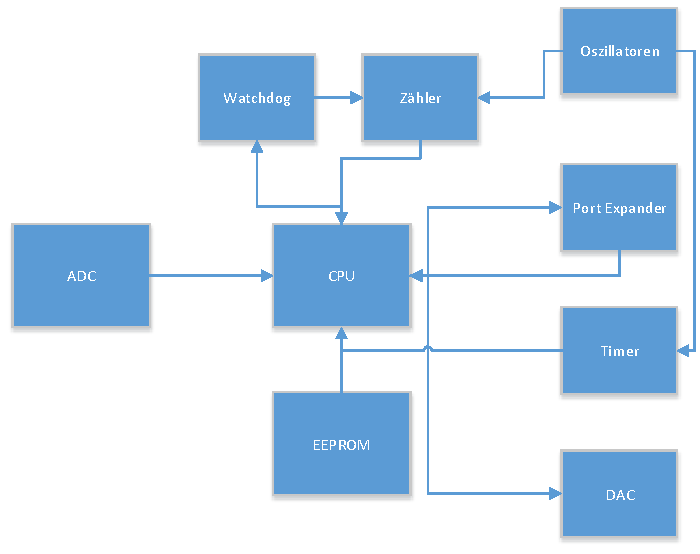
\includegraphics[scale=0.85]{ayoub/comparator_card_original.pdf}\\[3ex]
	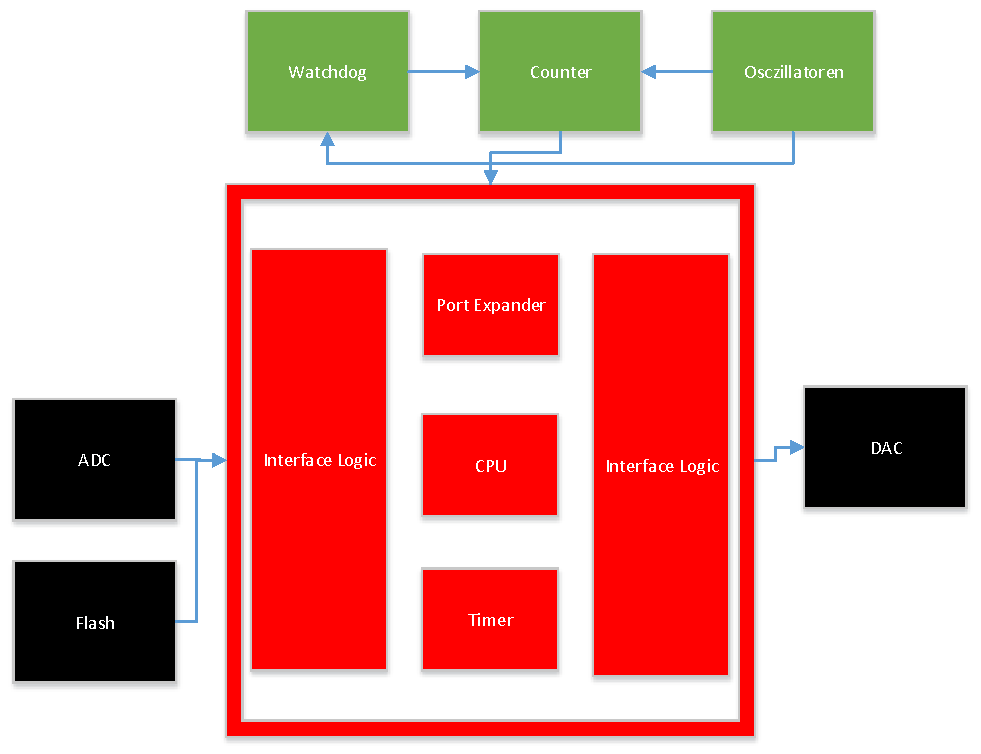
\includegraphics[scale=0.85]{ayoub/comparator_card_fpga.pdf}
	\caption[Block Diagrams of the Comparator Card]{Conceptual block diagrams of the comparator card: the original (top) and Ayoub's \gls{fpga}-based redesign (bottom), in which the red frame encloses the content of the \gls{fpga}, black elements are new and green ones were taken over from the original card. Reproduced as vector graphics from~\cite[Figs.~1 and~3]{ayoub2014}; the German labels are those of the original.}
	\label{fig:block_diagram_comparison}
\end{figure}

% the test setup is wide and its labels are small: it goes on a landscape page
\afterpage{%
\begin{landscape}
\begin{figure}[htbp]
	\centering
	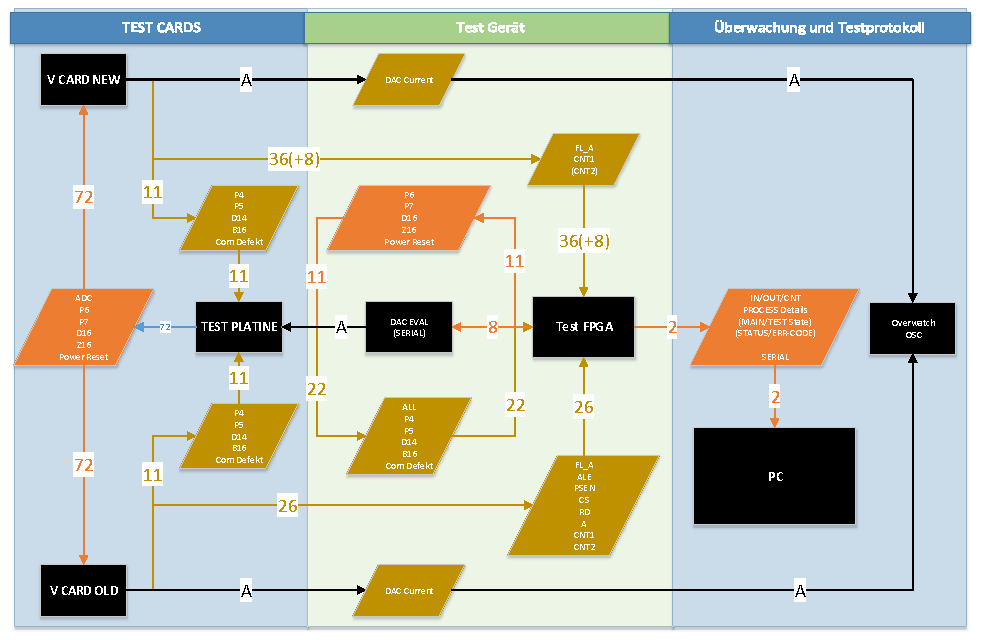
\includegraphics[height=0.82\textheight]{ayoub/test_setup.pdf}
	\caption[Ayoub Test Setup Concept]{Conceptual test setup for verifying the comparator card (German: \foreignlanguage{ngerman}{\textit{Vergleicherkarte}}) against the original, as documented in the preliminary work~\cite{ayoub2014}. Reproduced as a vector graphic from~\cite[Fig.~7]{ayoub2014}; the German labels are those of the original, and the three column headings are raster images in the original.}
	\label{fig:ayoub_test_setup}
\end{figure}
\end{landscape}}

\subsection{Test-Diagnosis Board Retrofit Attempt (Leyer)}
\label{subsec:leyer_internship}

Building on Ayoub's findings, Mark Leyer's 2023 internship project applied the~\gls{fpga} emulation strategy to the legacy system's test-diagnosis board~\cite{leyer2023}. This board, based on the 8035~\cite{leyer2023ppt}, the version of the 8048 without internal program memory~\cite[p.~1-2]{intel_mcs48_1978}, performs non-real-time diagnostics and self-test functions, including fault code storage and retrieval via a 7-segment display and initiation of a system self-test with frequency sweep output.

Leyer migrated the processor and its peripheral functions, namely the frequency sweep, the display driving, the button handling and the interface to the~\gls{nvram}, into~\gls{hdl} targeting an Actel ProASIC3 \texttt{A3P1000}~\gls{fpga}~\cite[Fig.~2]{leyer2023}, whose flash-based configuration memory is non-volatile, in contrast to alternatives based on~\gls{sram}.

Recognising the limitations of the legacy system's simple numeric code feedback, Leyer also designed an auxiliary diagnostics subsystem on a separate~\gls{pcb}~\cite{leyer2023, leyer2023ppt}. Centred on an~\gls{stm32} microcontroller (\texttt{STM32F401RET6}, \Cref{fig:schematic_sheet4}), the board was to provide modern data logging: errors timestamped via~\gls{rtc}, persistent storage on an~\gls{sd}~card and access over~\gls{usb}. A key design principle, critical for functional safety, was maintaining physical and electrical isolation between this non-safety-related logging function and the core safety-related~\gls{fpga} emulation, through an optocoupled~\gls{spi} link (\Cref{sec:stm32_details}).

While a single final test by Leyer showed the prototype behaving like the original system at start-up~\cite[Sec.~9.1]{leyer2023}, the prototype hardware (Rev~0.0) suffered from critical flaws that prevented robust operation. Subsequent hands-on debugging by a follow-on student project~\cite[pp.~10--14]{savchuk2025}, which continued the \texttt{test-diagnose} project and the capstone project \texttt{testkartentester24}, revealed that these were more extensive than initially documented, defining the true technical starting point for the hardware finalisation in this research. Examples of these inherited boards are shown in~\Cref{app:rev0_photos}.

\subsection{Challenges Encountered in Hardware Finalisation and Integration}
\label{subsec:hardware_challenges}

The starting point for this research was not just the design files, but a physical prototype that required significant analysis and rework to become a testable platform. The follow-on project~\cite[pp.~10--14]{savchuk2025} documented several latent issues that had to be overcome:

\begin{itemize}
	\item \textbf{Critical FPGA Soldering Defects:} The most significant hardware issue was the physical condition of the main \gls{fpga}. Supply and clock were present, checked with an oscilloscope, but the processor did not respond to reset and did not fetch from the Flash~\gls{rom}. What was initially thought to be a few poor connections was a systemic issue: four pins and then about 40 further pins on the \gls{fpga} required manual re-soldering~\cite[p.~13]{savchuk2025}; the \gls{fpga} was a used part desoldered from a broken board~\cite[Sec.~6.2]{leyer2023}. This underscores the gap between a lab prototype and a production-quality board; after the re-soldering, the unit could be switched on~\cite[p.~13]{savchuk2025}.
	\item \textbf{Fixture Debugging Interface:} The follow-on team could not debug the \gls{stm32} firmware of the test fixture, because pins needed by the~\gls{swd} interface had been assigned to~\gls{gpio}; they moved these functions to other pins, re-routed and re-soldered the affected tracks and revised the fixture \gls{pcb}~\cite[pp.~10, 12]{savchuk2025}. The \gls{stm32} Diagnostics Board of the retrofit routes \texttt{PA13}/\texttt{PA14} to its~\gls{swd} header \texttt{X14} in Rev~0.0 and Rev~1.0 alike (\Cref{fig:schematic_sheet4}).
	\item \textbf{Hardware Logic Errors:} When the rebuilt unit was tested on the fixture, it did not respond to the fixture's tests; debugging then revealed a logic error in the \gls{nvram} interface: the active-low byte-low-enable signal (\texttt{NVRAM\_ble}) was held high, which prevented correct access to the memory. After this was corrected in the \gls{vhdl}, the fixture's tests ran on the unit and the Lösch (clear) function worked again~\cite[p.~14]{savchuk2025} (\Cref{subsec:system_scenario_results}).
	\item \textbf{\gls{bom} Inaccuracies and Component Substitution:} The inherited~\gls{bom} required careful cross-referencing against schematics (\Cref{app:schematics}) and datasheets due to part number errors. Procurement difficulties necessitated substituting some non-standard components with standard parts (marked in \Cref{tab:bom}); no separate check of their equivalence is documented.
	\item \textbf{Documentation Fragmentation:} Foundational information was scattered across Ayoub's report~\cite{ayoub2014}, Leyer's documentation~\cite{leyer2023, leyer2023ppt}, and the original system manual~\cite{rexroth1992wsp}. Consolidating and verifying this information represented a significant initial overhead before design refinement could proceed.
\end{itemize}
These experiences highlight the importance of rigorously verifying all inherited artefacts and the physical hardware itself in continuation projects to mitigate risks of unforeseen delays.

% ------------------------------------------------------------
\section{Broader Context: Reverse Engineering and Obsolescence Management}
\label{sec:re_obsolescence}
The challenge of maintaining long-lifecycle systems reliant on obsolete components, such as the~\gls{mcs48} family in this project, arises wherever systems must stay in service for decades; Guzmán-Miranda et~al.\ describe it for the space and avionics domains~\cite{guzman2011obsolescence}, and the rail system studied here is another example. \Gls{re} provides techniques to understand and replicate legacy systems~\cite{wang2010}, and in safety-critical applications it requires particular rigour. Using~\glspl{fpga} for emulation is a recognised obsolescence management strategy~\cite{guzman2011obsolescence}, allowing legacy software retention while migrating hardware. As a case study, Guzmán-Miranda et~al.\ replace an obsolete Intel 8051 processor with one emulated on an \gls{sram}-based \gls{fpga} and use fault injection, with several application programs as workloads, to find the configuration bits whose upset makes those programs fail~\cite[Sec.~VII]{guzman2011obsolescence}. It is a precedent for the present retrofit, which emulates an~\gls{mcs48} processor on a flash-based \gls{fpga} and keeps its program unchanged (\Cref{sec:fpga_core_details}). A flash-based~\gls{fpga} (such as the Actel ProASIC3 \texttt{A3P1000} used here) has a configuration memory that is insensitive to the upsets (firm errors) affecting \gls{sram}-based devices~\cite{guzman2011obsolescence}; radiation data for the ProASIC3 family are reported in~\cite{poivey2011proasic3}. However, as this research illustrates, \gls{fpga} emulation necessitates thorough verification to ensure functional and timing equivalence, treating the~\gls{fpga} as a complex component requiring specific validation approaches (\Cref{chap:testing}).

\subsection{Verification Strategies for Functional Equivalence}
\label{subsec:equivalence_strategies}
While~\gls{re}~\cite{wang2010} and~\gls{fpga} emulation~\cite{guzman2011obsolescence} address hardware obsolescence, demonstrating \textit{functional equivalence} to the original system is essential, especially under safety standards such as~\gls{iec61508}~\cite{iec61508_2010} and~\gls{en50129}~\cite{en50129_2018}. In general terms, functional equivalence means identical behaviour and performance, particularly for safety functions and failure modes; the operational meaning in which this report uses the term is given in \Cref{subsec:requirement_basis}. Achieving certification-level confidence typically involves combining verification strategies:
\begin{description}
	\item[Black-Box System Testing:] Treats original and retrofit systems as black boxes, comparing outputs for identical inputs~\cite{ammann2016introduction}. This is effective for overall behaviour validation, but achieving full state and transition coverage via external interfaces alone is challenging for complex systems~\cite{hierons2009using}. \gls{hil} testing~\cite{hil_rail_suspension_2023, zhou_wu_2020} is a sophisticated variant common in rail, simulating the operational environment.
	\item[White-Box Analysis and Testing:] Utilised when internal details (legacy design documents, \gls{re} results, or new implementation specifics such as~\gls{hdl}) are available. Includes static analysis, code reviews, and structural testing~\cite{ammann2016introduction}. For hardware emulation, this demands detailed simulation, potentially formal verification~\cite{bozzano2016formal}, and ensuring \textit{timing equivalence}. Deviations in timing (e.g., instruction cycle duration, memory access latency, interrupt response time) can cause failures even with correct logic. Verification must target timing via cycle-accurate simulation, static timing analysis, and hardware measurements.
	\item[Formal Methods:] Employ mathematical models and proofs for verification. In railways they are applied mainly as model checking, simulation and theorem proving, most often to interlocking systems~\cite{formal_verification_rail_2023}. They offer high assurance but often require significant expertise and resources, with potential scalability limits~\cite{bozzano2016formal}. Sequential equivalence checking between two representations of a design, as used in digital design~\cite{mneimneh2005sequential}, might be adaptable to comparing a legacy design with its retrofit, but comparing microcontroller behaviour to an~\gls{fpga} implementation presents unique challenges.
	\item[Combined Approaches:] Practice often dictates combining strategies to leverage complementary strengths for safety-critical retrofits~\cite{ammann2016introduction}. White-box techniques (e.g., simulation) can verify component-level emulation logic, while black-box system testing (e.g., fixture-based tests, \gls{hil}) validates integrated behaviour. Such a layered approach contributes verification evidence towards a safety case; it is not a safety case by itself.
\end{description}
The verification methodology in this research (\Cref{chap:testing}) employs such a combined, two-layer strategy, integrating deterministic white-box checks (Layer~1: simulation, \gls{jtag} checks, timing measurement) with scenario-based system testing (Layer~2: fixture-based validation), a black-box approach that borrows from~\gls{hil} practice. How far its evidence for functional equivalence goes in this project is stated in \Cref{subsec:equivalence_discussion}.

% ------------------------------------------------------------
\section{Industry Practices and Related Work in Rail Retrofitting}
\label{sec:industry_practices}
Examining contemporary rail industry practices provides benchmarks for the feasibility of the methods used in this project.

\subsection{Benchmarks in WSP Modernisation and Certification}
\label{subsec:wsp_benchmarks}
Modernisation of~\gls{wsp} systems offers direct precedents. Wabtec's adaptive~\gls{wsp} function~\cite{wabtec_wsp_cert_2022} is particularly relevant: after laboratory tests at an accredited laboratory of DB Systemtechnik, tests on a test bench that simulated extremely low adhesion and a trial on an~\gls{sncf} Regiolis train, it was certified against~\gls{en15595} (editions 2011 and 2018)~\cite{en15595_2018}, and its use in the existing Regiolis fleet was announced. It shows that a new~\gls{wsp} function can \textit{achieve certification} against the current standard and is intended for existing fleets as well as for new trains. It is a benchmark for the certification pathway of this research (\Cref{sec:objectives_scope}), not evidence about this retrofit. Furthermore, \gls{hil} test benches for train braking and anti-skid have been built by railway operators and research institutes, as Zhou and Wu report with a design of their own~\cite[p.~155]{zhou_wu_2020}. While full~\gls{hil} was beyond this project's scope, the fixture-based testing approach (\Cref{sec:system_scenario_testing}) borrows from~\gls{hil} practice and could be a starting point for a later integration into a~\gls{hil} test rig (\Cref{sec:future_work}).

\subsection{Operational and Economic Drivers for Retrofitting}
\label{subsec:operational_economic_drivers}
Fleet upgrades illustrate the strategic motivations for retrofitting. The traction equipment of the former South West Trains Class~455 units, for example, was to be upgraded by replacing electro-mechanical control equipment and DC motors with solid-state inverters and AC traction motors, which were expected to have lower maintenance costs than the existing equipment~\cite{rg_class455_upgrade_2013}. By replacing ageing electronics, operators extend rolling stock life, deferring high capital expenditure for new trains, and lower maintenance reduces the overall~\gls{opex}. The Class~455 upgrade is one example of this motivation (\Cref{sec:context}); it says nothing about the costs of the present retrofit, which this report does not quantify (\Cref{sec:results_discussion_risk}).

% ------------------------------------------------------------
\section{Functional Safety Standards for Railway Systems}
\label{sec:standards_detail}
Ensuring safety in retrofits requires adherence to a framework of functional safety standards, which define the compliance objectives (\Cref{sec:objectives_scope}) and inform the verification methodology (\Cref{chap:testing}). Key applicable standards include:
\begin{description}
	\item[\gls{iec61508}~\cite{iec61508_2010}:] The foundational international standard for E/E/PE safety-related systems (Edition~2.0). Its Part~1 covers the aspects to be considered when E/E/PE systems are used to carry out safety functions, and Part~2 grades its techniques and measures for avoiding and controlling faults and failures against the~\gls{sil}~\cite{iec61508_2_2010}. This report draws on its Parts~2 and~3 for the~\gls{fpga} implementation, the reused program and the support tools (\Cref{sec:fpga_core_details,sec:verification_artefacts}).
	\item[\gls{en50126}:2017~\cite{en50126_1_2017, en50126_2_2017}:] Describes the RAMS life cycle of railway applications in two parts: Part~1 considers its generic aspects~\cite{en50126_1_2017}, and Part~2 gives guidance and methods that support the safety management process described in Part~1~\cite{en50126_2_2017}. \gls{en50129} and~\gls{en50716} below refer to it; this report does not apply it, and no RAMS or safety requirement has been derived for the module (\Cref{chap:safety_checklist}, item~CL-A4).
	\item[\gls{en50129}:2018~\cite{en50129_2018}:] Applies to safety-related electronic systems for railway signalling, from their specification to their modification and extension, and relies on the hazard analysis and risk assessment processes of~\gls{en50126} to identify the safety requirements~\cite{en50129_2018}. The module studied here is not a signalling system; this report draws on the standard's principles for safety-related electronic hardware by analogy, in particular for the~\gls{fpga} emulation. Its informative Annex~F gives guidance on user-programmable integrated circuits such as~\glspl{fpga}.
	\item[\gls{en50155}:2021~\cite{en50155_2021}:] Concerns, as its title says, electronic equipment on rolling stock; \gls{en61373}:2010~\cite{en61373_2010} concerns shock and vibration tests of rolling-stock equipment, and the~\gls{en50121} series (e.g.,~\cite{en50121_3_2_2016}) the~\gls{emc} of railway applications. Their texts were not read for this edition. They bear on the physical design choices (\Cref{sec:pcb_design_impl}), which have not been tested against them; type testing was out of scope.
	\item[\gls{en50716}:2023~\cite{en50716_2023}:] Specifies requirements for the development of software for programmable electronic systems in train control, train protection and signalling and on rolling stock, and applies only to software and its interaction with the system to which it belongs; it is aligned with \mbox{EN~50126-1} and \mbox{EN~50126-2}~\cite{en50716_2023} and supersedes EN~50128 and EN~50657. It applies to the~\gls{stm32} C firmware and to the reused 8048 object code executing on the soft core. The~\gls{hdl}/\gls{fpga} implementation itself is treated as hardware: under \mbox{\gls{iec61508}-2}, which covers the design and manufacture of E/E/PE safety-related systems except software~\cite{iec61508_2_2010}, and, for guidance, the informative Annex~F of~\gls{en50129} on user-programmable integrated circuits~\cite{en50129_2018}. Its description names support tools and firmware among its examples of application~\cite{en50716_2023}.
	\item[\gls{ieee1012}:2024~\cite{ieee1012_2024}:] Specifies verification and validation processes for systems, software and hardware, with life-cycle process requirements for different integrity levels~\cite{ieee1012_2024}. Following these processes is an objective of this work (\Cref{sec:objectives_scope}); the two-layer testing structure (\Cref{chap:testing}) and its artefacts (\Cref{sec:verification_artefacts,app:test_logs,app:test_cases}) were not set up as a~\gls{vv} plan in the sense of the standard, and no integrity level has been assigned (\Cref{sec:safety_compliance}).
\end{description}
Applying these standards to retrofits requires demonstrating that modifications do not compromise existing safety levels and that new elements are adequately verified. This involves impact analysis, configuration management, and regression testing. \gls{en50129} covers the modification of the systems in its scope and, as far as reasonably practicable, of systems accepted before it~\cite{en50129_2018}; \gls{en50716} covers only the software side of a modification, here the reused program and the~\gls{stm32} firmware, and not the replacement of the controller hardware. \Cref{sec:en50716_modifications} describes how far the methodology addresses them in this project: no impact analysis is documented, and the regression tests and the configuration management are incomplete.

The vehicle of this case is an urban-rail car (Stadtbahnwagen~B~\cite{rexroth1992wsp}). In Germany, the construction and operation of tramways in the sense of \S~4 of the Passenger Transport Act (PBefG) are governed by the BOStrab~\cite[\S~1]{bostrab}; which approval route would apply to this retrofit has not been examined. The published scope of~\gls{en15595} excludes vehicles with rubber tyres and vehicles with hydraulic brakes~\cite{en15595_2018}. The manual describes the anti-skid control valves acting on a pneumatic brake: its functional check commands the pneumatic brake and checks the valves by the pressure in the C pipe~\cite[Blatt~17/25, 18/25]{rexroth1992wsp}. Whether the standard applies to the vehicle of this case has not been examined beyond this.

\subsection{FPGA-Specific Certification Considerations}
\label{subsec:fpga_certification}
Using~\glspl{fpga} in safety-critical retrofits, while addressing obsolescence~\cite{guzman2011obsolescence}, introduces specific certification considerations compared to traditional controllers:
\begin{itemize}
	\item \textbf{Development Tool Confidence:} Complex~\gls{fpga} tools (synthesis, place-and-route) may need a justification for safety-related use, through tool qualification or diverse verification measures. Because the~\gls{hdl} is treated as hardware here (\Cref{sec:standards_detail}), \gls{en50716}, which applies only to software~\cite{en50716_2023}, does not cover these tools; which requirements of the hardware standards apply to them has not been examined, and the tools of this project have not been assessed (\Cref{sec:verification_artefacts}).
	\item \textbf{Hardware Verification:} The implemented logic needs rigorous verification; \gls{en50129} has an informative annex on user-programmable integrated circuits~\cite{en50129_2018}. This involves extensive simulation, potentially formal methods~\cite{formal_verification_rail_2023}, and hardware testing to confirm behaviour and address potential~\gls{fpga} fabric failure modes. Flash-based~\glspl{fpga}, such as the ProASIC3 used (\texttt{A3P1000}), are less susceptible to configuration memory upsets than \gls{sram}-based alternatives~\cite{guzman2011obsolescence, poivey2011proasic3}.
	\item \textbf{Pre-Developed IP Validation:} Using third-party or open-source~\gls{ip}, such as the~\gls{mcs48} core (\Cref{sec:fpga_core_details}), necessitates thorough verification and validation by the integrator, as prior safety certification is often lacking. Demonstrating functional and timing equivalence within the application context is essential.
\end{itemize}
Addressing these points is key to building the safety case for an~\gls{fpga}-based safety-critical retrofit.

% ------------------------------------------------------------
\section{Relevant Design and Manufacturing Principles}
\label{sec:design_principles}
The hardware architecture and physical design choices detailed in~\Cref{chap:architecture} were guided by established principles for reliable railway electronics and by the design guidelines applicable to the project; these principles state aims, and the system has not been tested against the standards named below:
\begin{description}
	\item[PCB Layout Practices~\cite{jones2004}:] Careful~\gls{pcb} layout is fundamental. Key practices applied include strategic component placement, appropriate trace widths (impedance and current, following guidelines such as those in~\cite[pp.~7, 10, 12]{jones2004}), clearances set by the manufacturer's rule set (\Cref{sec:app_drc}), grounding with ground planes, and decoupling capacitors close to~\glspl{ic} to ensure signal integrity and minimise noise~\cite[Sec.~Tracks, Pads, Clearances, Grounding, Bypassing]{jones2004}. Rules regarding vias, trace angles (45-degree preferred over 90-degree), and pad extensions for manual soldering were also considered.
	\item[Electromagnetic Compatibility (\gls{emc}/\gls{emi}):] Railway environments call for robustness against electromagnetic noise. The~\gls{emc} of rolling-stock apparatus is the subject of \mbox{EN~50121-3-2}~\cite{en50121_3_2_2016}. The measures of this design that bear on~\gls{emc} are the ground planes, the decoupling and the galvanic isolation of the~\gls{spi} link~\cite{ott2009emc} (\Cref{sec:pcb_design_impl}); no~\gls{emc} test of the design has been made.
	\item[DFM and Reliability:] {\sloppy Addressing previous~\gls{dfm} issues~\cite{leyer2023} (\Cref{subsec:leyer_internship}) was a primary goal. By their titles, \gls{en50155}~\cite{en50155_2021} concerns the electronic equipment of rolling stock and \gls{en61373}~\cite{en61373_2010} shock and vibration tests of rolling-stock equipment; their texts were not read for this edition. No component of this design is documented as selected for them, and no test against them has been made (\Cref{sec:validation_context}). Adherence to the project's design rules contributes to manufacturability.\par}
	\item[Modularity and Isolation:] The modular design, with its Base, Upper, \gls{stm32} and \gls{led} boards, enhances testability, maintainability, and fault isolation. Galvanic isolation of the~\gls{spi} link (\Cref{sec:stm32_details}) is meant to keep faults on the isolated, non-safety-related side (\gls{stm32} diagnostics) from feeding back into the safety-related (\gls{fpga}) domain; the parts of the \gls{stm32} Diagnostics Board on the other side of the barrier share the supply of the Base Board (\Cref{sec:stm32_details}).
	\item[Supervision and Fail-Safe Concepts:] A fail-safe concept detects failures and brings the system into a safe state; \mbox{\gls{iec61508}-2} requires techniques and measures for the control of faults and failures, graded against the safety integrity level~\cite{iec61508_2_2010}. Full hardware redundancy was out of scope, and two supervision features were included (\Cref{sec:redundancy_failsafe}): an independent hardware watchdog, kept as on the original board, monitors the activity of the emulated controller, and a~\gls{bod} supervisor, added in the retrofit~\cite[Sec.~2]{leyer2023}, monitors its supply rails. Both hold the emulated controller in reset when they detect a fault; since no safe state has been derived for the module, this reset is not shown to be a safe state (\Cref{sec:vehicle_outputs}). The system also retains its legacy self-test capabilities, which contribute to fault detection.
\end{description}

% ============================================================
% Chapter 3: System Architecture and PCB Design
% ============================================================
\chapter{System Architecture and PCB Design}
\label{chap:architecture}

This chapter details the technical implementation of the retrofitted test-diagnosis module, translating the design principles discussed in~\Cref{sec:design_principles} into a concrete hardware architecture. The system employs a modular design across four distinct~\glspl{pcb} to enhance isolation, testability, and maintainability, reflecting common practice for complex electronic systems. Detailed schematics and layout diagrams are provided in~\Cref{app:schematics}.

% ------------------------------------------------------------
\section{System Architecture Overview}
\label{sec:overall_architecture}

\begin{figure}[htbp]
	\centering
	% High-level block diagram of the retrofitted test-diagnosis system.
% Kept as diagram source rather than a bitmap so that it diffs, reviews and
% rebuilds deterministically with the rest of the document. Derived from the
% block diagram of the published paper; the RTC node names the STM32's internal
% RTC with its 32.768 kHz crystal, which is what the Rev 1.0 schematic and layout
% show. The board assignment follows the Rev 1.0 Eagle layouts: the BOD
% supervisor (Y3) and the CD4050 level shifters for the X4 inputs sit on the Base
% Board, the watchdog (Y4, Y5, Q1) and the debouncing (Y6) on the Upper Board.
% The BOD output drives the watchdog's reset transistor Q1 over X9/X8, so its
% reset reaches the FPGA through the Upper Board. The outputs to the system
% connector X4 leave the Base Board through the 54LS245-type drivers Y8 and Y12
% (schematic sheets 2 and 3); their arrow leaves the board below the LED Board.
% Edge labels sit on the side of their arrow away from the neighbouring label,
% and the STM32 peripherals stand far enough from the STM32 for a visible arrow.
% The 5 V supply and ground of the Base Board reach the Diagnostics Board through
% X13/X12 (schematic sheet 4); on the Base Board side of the barrier the 5 V (net
% PWR_SUPPLY_5V) feeds only the suppressor diode D16 and the input of the isolated
% converter Y23 (the footprint Y22 is unfitted), drawn as the dark arrow. The LEDs of
% the optocouplers share only the ground (GND3) and are driven by the logger and
% reset lines through R82-R85 (X12 pins 2-5); the branch is their ground return.
% The FPGA reaches the NVRAM over address, data and enable lines (atop.vhd, Rev 1.0
% schematic: A0-A5, DQ0-DQ7, CE, OE, WE, BLE); the fitted NVRAM needs no STORE and
% RECALL, and the X4 STORE/RECALL inputs feed only the logger.
\resizebox{\textwidth}{!}{%
\begin{tikzpicture}[
    module/.style={draw, thick, rounded corners=3pt, minimum width=2.6cm,
                   minimum height=1.2cm, align=center, font=\small},
    fpga/.style={draw, very thick, rounded corners=5pt, minimum width=5.6cm,
                 minimum height=4cm, align=center, font=\normalsize\bfseries,
                 fill=gray!5},
    pcb/.style={draw, thick, rounded corners=8pt, inner sep=14pt},
    pcblabel/.style={font=\small\bfseries\sffamily, fill=white, inner sep=3pt},
    conn/.style={-{Stealth[length=2.5mm]}, thick},
    bconn/.style={{Stealth[length=2.5mm]}-{Stealth[length=2.5mm]}, thick},
    isoconn/.style={-{Stealth[length=2.5mm]}, very thick, densely dashed, red!70!black},
    pwrconn/.style={-{Stealth[length=2.5mm]}, very thick, black!75},
    lbl/.style={font=\scriptsize, midway, fill=white, inner sep=1.5pt},
  ]
  \node[fpga] (fpga) at (0,0) {FPGA\\{\small Actel A3P1000-PQG208M}\\[3pt]{\footnotesize\itshape MCS-48 Emulation\/}};

  \node[module, fill=gray!4] (pwr)   at (-7.5, 1.0) {Power Supply\\{\footnotesize \SI{3.3}{\volt} / \SI{1.5}{\volt}}};
  \node[module, fill=gray!4] (flash) at (-3.5, 3.5) {Flash ROM\\{\footnotesize S29AL016J}};
  \node[module, fill=gray!4] (xtal)  at (0, 3.5)    {Crystal\\{\footnotesize \SI{6}{\mega\hertz}}};
  \node[module, fill=gray!4] (nvram) at (3.5, 3.5)  {NVRAM\\{\footnotesize CY14B104NA}};
  \node[module, fill=gray!4] (bod)   at (-7.5, -1.3) {BOD\\{\footnotesize TPS3307}};
  \node[module, fill=gray!4] (jtag)  at (-7.5, 3.5)  {JTAG\\{\footnotesize Debug}};
  \node[module, fill=gray!4, minimum height=1.0cm] (lvl) at (5.6, -0.2) {Level Shift\\{\footnotesize CD4050}};
  \node[module, fill=gray!4, minimum height=1.0cm] (drv) at (5.6, -1.8) {Output Drivers\\{\footnotesize 54LS245-type}};
  \node[module, fill=gray!4] (freq)  at (-3.5, -3.5){Freq.\ Sweep\\{\footnotesize \SI{850}{\hertz}--\SI{1550}{\hertz}}};
  \node[module, fill=gray!4] (spi)   at (0, -3.5)   {SPI Master\\{\footnotesize (32-bit frames, 2023)}};
  \node[module, fill=gray!4] (ioexp) at (3.5, -3.5) {I/O \& Port\\{\footnotesize Expander}};

  \node[module, fill=green!8] (bcd)  at (9.3, 0.8)  {BCD Decoder\\{\footnotesize CD4511BE}};
  \node[module, fill=green!8] (disp) at (12.8, 0.8) {7-Segment\\{\footnotesize Displays ($\times 2$)}};

  \node[module, fill=blue!8] (wd)       at (-7.5, -6.5) {Watchdog\\{\footnotesize CD40106, CD4518}};
  \node[module, fill=blue!8] (btns)     at (-7.5, -8.5) {Buttons\\{\footnotesize Test, STW, L\"osch, T\"ur/V}};
  \node[module, fill=blue!8] (debounce) at (-3.5, -8.5) {Debounce};

  \node[module, fill=orange!10] (opto) at (3.5, -7)   {Optocouplers\\{\footnotesize SFH601-3 ($\times 4$)}};
  \node[module, fill=orange!10] (stm)  at (7, -7)     {STM32\\{\footnotesize F401RET6}};
  \node[module, fill=orange!10] (rtc)  at (10.8, -5.5)  {RTC\\{\footnotesize internal, \SI{32.768}{\kilo\hertz}}};
  \node[module, fill=orange!10] (sd)   at (10.8, -7)    {MicroSD\\{\footnotesize (FatFs)}};
  \node[module, fill=orange!10] (usb)  at (10.8, -8.5)  {USB\\{\footnotesize Type-C}};
  \node[module, fill=orange!10] (pwrin) at (0.6, -7) {D16, Y23 input\\{\footnotesize Base Board side}};

  \begin{scope}[on background layer]
    \node[pcb, draw=gray!50, fill=gray!2,
          fit=(fpga)(pwr)(flash)(xtal)(nvram)(bod)(jtag)(lvl)(drv)(freq)(spi)(ioexp)] (bb) {};
    \node[pcb, draw=green!40!black, fill=green!2, fit=(bcd)(disp)] (lb) {};
    \node[pcb, draw=blue!40!black, fill=blue!2, fit=(wd)(btns)(debounce)] (ub) {};
    \node[pcb, draw=orange!50!black, fill=orange!2, fit=(opto)(stm)(rtc)(sd)(usb)(pwrin)] (sb) {};
  \end{scope}

  \node[pcblabel, text=gray!60] at (bb.north) {PCB 1: Base Board};
  \node[pcblabel, text=green!40!black] at (lb.north) {PCB 4: LED Board};
  \node[pcblabel, text=blue!40!black] at (ub.south) {PCB 2: Upper Board};
  \node[pcblabel, text=orange!50!black] at (sb.south) {PCB 3: STM32 Diagnostics Board};

  \draw[conn] (pwr.east) -- node[lbl, above] {\SI{1.5}{\volt}} (pwr.east -| fpga.west);
  \draw[conn] (pwr.south) -- node[lbl, right] {\SI{3.3}{\volt}} (bod.north);
  \draw[conn] (bod.south) -- node[lbl, right] {Reset} (wd.north);
  \draw[bconn] (wd.east) -| (-5.45, -0.5) -- node[lbl, above] {Reset / !CS} (fpga.west |- 0, -0.5);
  \draw[conn] (jtag.east) -- ++(0.8, 0) |- (fpga.west |- 0, 1.6);
  \draw[conn] (lvl.west) -- node[lbl, above] {X4 inputs} (lvl.west -| fpga.east);
  \draw[conn] (drv.west -| fpga.east) -- (drv.west);
  \draw[conn] (drv.east) -- node[lbl, above] {X4 outputs} ++(1.9, 0);
  \draw[bconn] (flash.south) -- node[lbl, below left] {Firmware} ([xshift=-1.5cm]fpga.north);
  \draw[conn] (xtal.south) -- node[lbl, left] {CLK} (fpga.north);
  \draw[bconn] (nvram.south) -- node[lbl, below right] {Address / Data} ([xshift=1.8cm]fpga.north);
  \draw[conn] (fpga.240) -- (freq.north);
  \draw[conn] (fpga.south) -- (spi.north);
  \draw[bconn] ([xshift=1.8cm]fpga.south) -- (ioexp.north);
  \draw[conn] (fpga.east |- bcd.west) -- node[lbl, above, pos=0.3] {BCD} (bcd.west);
  \draw[conn] (bcd.east) -- (disp.west);
  \draw[conn] (btns.east) -- (debounce.west);
  \draw[conn] (debounce.north) |- (-5.05, -5.0) |- (fpga.west |- 0, -1.5);
  \draw[isoconn] (spi.south) -- ++(0,-1) -| node[lbl, right, text=red!70!black, font=\scriptsize\bfseries, pos=0.25] {Galvanic Isolation} (opto.north);
  \draw[conn] (opto.east) -- node[lbl, above] {SPI} (stm.west);
  \draw[bconn] (stm.north) |- (rtc.west);
  \draw[bconn] (stm.east) -- (sd.west);
  \draw[bconn] (stm.south) |- (usb.west);
  \coordinate (feedx) at (-0.3, 0);
  \coordinate (ledx) at (2.6, 0);
  \coordinate (branch) at (-0.3, -5.75);
  \draw[pwrconn] (bb.south -| feedx) -- node[lbl, left, pos=0.2] {\SI{5}{\volt}, GND} (pwrin.north -| feedx);
  \draw[pwrconn] (branch) -| node[lbl, below, pos=0.3] {GND} (opto.north -| ledx);
  \fill[black!75] (branch) circle (2pt);
\end{tikzpicture}%
}

	\caption[High-Level Block Diagram of the Retrofitted System]{High-level block diagram of the retrofitted test-diagnosis module. Four boards are shown: the Base Board with the \gls{fpga} core and the drivers of the outputs to the system connector \texttt{X4} (grey), the Upper Board with the operator controls and the watchdog (blue), the LED Board (green), and the galvanically isolated \gls{stm32} Diagnostics Board (orange). The dashed red arrow, labelled Galvanic Isolation, marks the \gls{spi} link from the \gls{spi} master to the optocouplers of the \gls{stm32} Diagnostics Board. The dark arrow carries the \SI{5}{\volt} supply and the ground of the Base Board through \texttt{X13}/\texttt{X12} to the parts of the \gls{stm32} Diagnostics Board on the Base Board side of the barrier; its branch, labelled GND, is the ground return of the optocoupler \glspl{led} (\Cref{sec:stm32_details}). Adapted from~\cite[Fig.~1]{torun2026}; the figure stays under the licence of the Working Paper, \mbox{CC~BY-NC-ND~4.0}.}
	\label{fig:overall_system}
\end{figure}

The retrofitted system comprises four boards (\Cref{fig:overall_system}) designed to collaboratively replicate and enhance the functionality of the original test-diagnosis module:

\begin{description}
	\item[Base Board (Unterplatine):] The central processing hub housing the Actel \texttt{A3P1000-\allowbreak PQG208M}~\gls{fpga} (\Cref{fig:schematic_sheet1}, designator \texttt{Y20} in~\Cref{tab:bom}) running the emulated~\gls{mcs48} core. The ProASIC3 family has a non-volatile, flash-based configuration memory that is insensitive to the configuration-memory upsets (firm errors) affecting \gls{sram}-based devices~\cite{guzman2011obsolescence}; radiation data for the family are reported in~\cite{poivey2011proasic3}. This board integrates the support circuitry, including power regulation (\texttt{Y1}, \texttt{Y2}), the \SI{6}{\mega\hertz} clock generation (\texttt{Q6}, \texttt{Y16}, \Cref{fig:schematic_sheet2}), \gls{nvram}~(\texttt{Y15}, \texttt{CY14B104NA}, \Cref{fig:schematic_sheet2}) for non-volatile storage of fault codes, the \gls{bod} supervisor (\texttt{Y3}, \Cref{fig:schematic_sheet1}), a~\gls{jtag} header (\texttt{X3}) for programming and debugging, and the necessary inter-board connectors (\texttt{X5}/\texttt{X6}, \texttt{X9}, \texttt{X13}). It also houses the interface to the system connector \texttt{X4}: CD4050 level shifters for its inputs (\texttt{Y7}, \texttt{Y9}--\texttt{Y11}, \texttt{Y17}) and 54LS245-type drivers for its outputs (\texttt{Y8}, \texttt{Y12}). The schematic is given in~\Cref{sec:app_schematic_sheets} and the layout in~\Cref{sec:app_base_board_schematics} (\Cref{fig:base_layout_top,fig:base_layout_bottom}). The Base Board layout shown corresponds to the inherited Rev~0.0 board, which was reused after rework (\Cref{subsec:hardware_challenges}).

	\item[Upper Board (Oberplatine):] Carries the operator interface and the supervision of the controller: the four legacy buttons (\texttt{S1}--\texttt{S4}) with their debouncing (\texttt{Y6}, \Cref{fig:schematic_sheet2}) and the external watchdog with its reset circuit (\texttt{Y4}, \texttt{Y5}, \texttt{Q1}, \Cref{fig:schematic_sheet1}). The buttons are those of the legacy front panel~\cite[Blatt~5/25]{rexroth1992wsp}: Test starts the self-test, \gls{stw} the fault query (\emph{Störstellen-Abfrage}), which shows the stored fault information entry by entry, and Lösch (clear) erases it. The button labelled \gls{tuerv} in the design files, V-SIGN on that panel, lets the speed-dependent signals be checked at standstill without the complete test sequence~\cite[Blatt~14/25, 19/25]{rexroth1992wsp}. It is connected to the Base Board by a ribbon cable between the headers \texttt{X8} and \texttt{X9}. The layout (Rev~1.0, designed by Leyer~\cite{leyer2023}) is shown in~\Cref{sec:app_upper_board_schematics} (\Cref{fig:upper_layout_top,fig:upper_layout_bottom}).

	\item[STM32 Diagnostics Board:] (\Cref{fig:schematic_sheet4}) This separate board provides enhanced diagnostic and logging capabilities, intentionally decoupled from the safety-critical anti-skid core logic using galvanic isolation. It features an \texttt{STM32F401RET6} microcontroller (\texttt{Y24}, Arm\textsuperscript{\textregistered}~Cortex\textsuperscript{\textregistered}-M4), chosen for its suitable peripheral set (\gls{spi}, \gls{sdio}, \gls{usb}, \gls{rtc}) and processing capability for the logging task, aligning with hardware used in the test fixture development~\cite{dolata2023}. Timestamps come from the microcontroller's internal~\gls{rtc}, clocked by a \SI{32.768}{\kilo\hertz} crystal (\texttt{Q8}) and backed by a CR2032 cell in holder \texttt{U1} (\texttt{BS-7}); an~\gls{sdio} interface to a MicroSD card (\texttt{J6}) provides persistent logging using FatFs, and a~\gls{usb} Type-C interface (\texttt{X15}) serves data retrieval. Communication with the Base Board~\gls{fpga} occurs via a galvanically isolated~\gls{spi} link (optocouplers \texttt{OK5}--\texttt{OK8}), which is meant to keep faults on the isolated side out of the \gls{fpga} domain (\Cref{sec:design_principles}); the parts of the board on the Base Board side of the barrier are not covered by it (\Cref{sec:stm32_details}). An isolated DC/DC converter (\texttt{Y23}; the footprint \texttt{Y22} is an unpopulated alternative) and a \SI{3.3}{\volt} low-dropout regulator (\texttt{Y19}, \texttt{TPS73633}) supply the isolated domain. The introduction of~\gls{usb} and~\gls{sd} interfaces necessitates future cybersecurity assessment (\Cref{sec:future_work}). See~\Cref{sec:app_stm32_board_schematics} (\Cref{fig:stm32_layout_top,fig:stm32_layout_bottom} for the Rev~1.0 layout).

	\item[LED Board:] Houses the two physical 7-segment~\gls{led} displays (\texttt{DS1}, \texttt{DS2}, Kingbright \texttt{SC03-12EWA}~\cite{kingbright2020}) showing the user the codes of \Cref{tab:requirement_basis} (e.g., 99 for no fault, 88 for the lamp test, 31 in the read-out of a sensor fault), driven by two driver ICs that decode~\gls{bcd} to 7-segment signals (\texttt{Y13}/\texttt{Y14}, \texttt{CD4511BE}). It plugs directly onto the Base Board (\texttt{X10}/\texttt{X11} into \texttt{X5}/\texttt{X6}). The schematic is part of \Cref{fig:schematic_sheet3}, and the layout (Rev~1.0) is shown in~\Cref{sec:app_led_board_schematics} (\Cref{fig:led_layout_top,fig:led_layout_bottom}).
\end{description}

In this report, \emph{the rebuilt unit} denotes the test-diagnosis module as rebuilt: the inherited Rev~0.0 Base Board with the Rev~1.0 Upper, LED and \gls{stm32} boards.

Physical interconnection utilises direct board-to-board mounting (LED Board onto Base Board via \texttt{X5}/\texttt{X6}; \gls{stm32} Diagnostics Board onto Base Board via \texttt{X13}) and cabled connections (Base Board to Upper Board via a ribbon cable between \texttt{X9} and \texttt{X8} for the button, interrupt and reset signals). This modular approach enhances testability and maintainability, fulfilling a key design principle (\Cref{sec:design_principles}). Leyer found the footprints of \texttt{X5} and \texttt{X6} on the Rev~0.0 Base Board wrong, because the connectors have pins of two sizes; on the prototype he bridged them with short wires, which he called an unstable solution, and he corrected the footprints in the Rev~1.0 layout~\cite[Sec.~9.2]{leyer2023}. The reused Base Board is Rev~0.0 and keeps these footprints; how the LED Board was connected to it on the rebuilt unit is not documented. Reusing previously modified hardware calls for an incoming inspection; apart from the inspection of the populated boards for the~\gls{bom}, none is documented for the rebuilt unit (\Cref{chap:safety_checklist}, item~CL-F2). Connector details are given in~\Cref{sec:app_connectors}.

\subsection{Outputs to the Vehicle}
\label{sec:vehicle_outputs}

The module acts on the vehicle only through the outputs of the system connector \texttt{X4}, which the 54LS245-type drivers \texttt{Y8} and \texttt{Y12} drive, some through series resistors and three through the transistors \texttt{Q3}--\texttt{Q5} (\Cref{fig:schematic_sheet2,fig:schematic_sheet3}). The fixture report names them: four frequency outputs to the axle cards (pins 12z, 10d, 12d and 12b), the outputs \enquote{AV-Sperre} A1 to A4 (16d, 14z, 14b, 14d) and \enquote{V-Test} (04d)~\cite[Sec.~5.1.5, 5.2]{dolata2023}. In the self-test, the module sends a frequency sweep to each of the four axle cards in turn~\cite[Sec.~5.1.5]{dolata2023}, which simulates a misbehaviour so that the axle cards' recognition of sliding can be tested~\cite[Sec.~2.9]{leyer2023}. According to the manual, the anti-skid control valves then act one after another, which is checked with a pressure gauge on the C pipe~\cite[Blatt~18/25]{rexroth1992wsp}. The check, according to the manual, runs automatically after the supply is switched on, or at standstill when the Test button is pressed with the braking signal present, and the spring-applied brake is to be applied for it~\cite[Blatt~14/25]{rexroth1992wsp}; the V-SIGN button is to be pressed only at standstill~\cite[Blatt~19/25]{rexroth1992wsp}. What the outputs AV-Sperre and V-Test act on in the vehicle is not described in these sources; the state of all outputs during power-up and during a watchdog or brown-out reset is not documented; and what prevents a self-test, with its sweep and valve actions, while the vehicle is moving is documented only as these instructions of the manual. Whether a reset by the watchdog or the \gls{bod} circuit in service leads the unchanged program into the automatic check that the manual describes after switching on, with its valve actions, has not been examined; it is an open question for a hazard analysis (\Cref{chap:safety_checklist}, item~CL-A4).

No safety function, no~\gls{sil} target and no safe state has been derived for the module (\Cref{chap:safety_checklist}, item~CL-A4). Where this report calls the emulated core \enquote{safety-related} or \enquote{safety-critical}, the words describe the intent of the design, not a classification.

% ------------------------------------------------------------
\section{FPGA Core Implementation Details}
\label{sec:fpga_core_details}

The core logic resides in the \texttt{A3P1000}~\gls{fpga} and is implemented in~\gls{vhdl}. The \gls{vhdl} sources (among them \texttt{atop.vhd}, \texttt{t48\_core.vhd}, \texttt{t8243\_sync\_notri.vhd}, \texttt{sweep\_top.vhd} and \texttt{Logger\_top.vhd}), the \gls{stm32} firmware and the fixture's test cases are not published with this report. \Cref{app:test_cases} gives only an adapted version of one \gls{yaml} test case of the fixture~\cite[Listing~3]{dolata2023}, in two steps, and reproduces one excerpt of twelve lines from \texttt{atop.vhd}.

\begin{description}
	\item[MCS-48 Emulation Core:] An emulation of the \gls{mcs48} processor serves as the central processing element. According to its original schematic, the legacy board carries a ROM-less member of the family (an \texttt{INS8035NI}; the schematic also names an NEC \texttt{D80C39HC}), which fetched its program from an external~\gls{eprom}. Following Leyer's approach~\cite{leyer2023}, an existing implementation (\texttt{t48\_core.vhd}) from the OpenCores repository\footnote{OpenCores website: \url{https://opencores.org/}. Validation of the specific core used relies on project testing.} was integrated unmodified. This core executes the original firmware, read from the Flash~\gls{rom} that replaced the~\gls{eprom}, preserving the legacy control logic and aiming at behavioural compatibility at the instruction level. The design history of the binary is not available. Its reuse rests on the service of the original module since the early 1990s (\Cref{chap:introduction}); no operational data are cited, and which evidence \mbox{\gls{iec61508}-3}~\cite{iec61508_3_2010} would require for reusing it has not been examined. The primary verification challenge lies in ensuring that this emulation is functionally and temporally equivalent to the original hardware within the target application's constraints (\Cref{subsec:equivalence_strategies,subsec:fpga_certification}).
	\item[Memory Interfaces:] The~\gls{fpga} implements the logic to interface directly with the external memory components located on the Base Board: an \texttt{S29AL016J} Flash~\gls{rom} (\texttt{Y21}) storing the executable firmware, and a \texttt{CY14B104NA}~\gls{nvram} (\texttt{Y15}) used for persistent storage of fault codes (\Cref{fig:schematic_sheet1,fig:schematic_sheet2}). The~\gls{fpga} generates the required address, data, and control signals (chip enable, output enable, write enable, byte enables) according to the timing requirements of these memory devices and the access patterns dictated by the emulated~\gls{mcs48} core. Checking the timing on these interfaces is part of Layer~1 verification (\Cref{sec:fpga_interface_testing}).
	\item[Peripheral Emulation and Interfaces:] The~\gls{fpga} logic replicates or interfaces with the essential peripherals of the legacy test-diagnosis board:
	      \begin{itemize}
		      \item \textit{7-Segment Display Driving Logic:} Generates the~\gls{bcd} signals and the latch enable (\texttt{FPGA\_7SEG\_LE}; at the drivers \texttt{CON\_7SEG\_LE}) required by the external \texttt{CD4511BE} display drivers located on the LED Board (\Cref{fig:schematic_sheet3}).
		      \item \textit{Input Button Handling:} The STW and Lösch buttons reach the emulated core directly on \texttt{T0} and \texttt{T1}; the Test and Tür/V buttons reach \texttt{P10}/\texttt{P11} and, combined on the Upper Board, the interrupt lines \texttt{!INT\_A}/\texttt{!INT\_B}, which the \gls{fpga} merges into the core's interrupt input~\cite{leyer2023} (\Cref{fig:schematic_sheet2}).
		      \item \textit{Frequency Sweep Generation:} A digital generator (\texttt{freq\_gen.vhd}, \path{sweep_top.vhd}) replaces the original analogue circuit based on a~\gls{vco}. It divides the \SI{6}{\mega\hertz} system clock by a factor taken from a lookup table,
		      \begin{equation}
			      f_\mathrm{out}(i) = \frac{f_\mathrm{clk}}{2 \cdot (N_\mathrm{div}(i) + 1)}, \qquad f_\mathrm{clk} = \SI{6}{\mega\hertz},
			      \label{eq:sweep}
		      \end{equation}
		      where an internal \SI{600}{\hertz} clock (\texttt{gen600Hz.vhd}) steps through the table and so produces a non-linear sweep profile. Each half period lasts $N_\mathrm{div} + 1$ cycles of the system clock, because the counter in \texttt{freq\_gen.vhd} counts from 0 up to $N_\mathrm{div}$ before the output toggles. $N_\mathrm{div}$ ranges from 1935 ($f_\mathrm{out} \approx \SI{1549.6}{\hertz}$) to 3529 ($f_\mathrm{out} \approx \SI{849.9}{\hertz}$); the table for the rising sweep has 33 entries and the table for the falling sweep 65 entries, so the sweeps cover \SI{850}{\hertz} to \SI{1550}{\hertz} and back, the values Leyer gives for the sweep of the original board~\cite[Sec.~2.9]{leyer2023}. The generator advances by one entry per period of the \SI{600}{\hertz} clock, which \texttt{gen600Hz.vhd} derives from the system clock by toggling its output every 5000 cycles, so the rising sweep reaches its end value after 31 steps, about \SI{52}{\milli\second}, and the falling sweep after 61 steps, about \SI{102}{\milli\second}; the tables end after 32 and 64 steps. Leyer reports that he checked the end frequencies, the duration and the profile of the sweep against the original board, without giving values~\cite[Sec.~4.10]{leyer2023} (\Cref{fig:sweep_comparison}); the captures read about \SI{920}{\hertz} at the low end of the original board, and the fixture report gives about \SI{180}{\milli\second} for the frequency change of the original test card (\Cref{subsec:fpga_interface_results}).
		      \item \textit{\gls{spi} Master Interface:} Implements an~\gls{spi} master (\texttt{Logger\_top.vhd}, \path{SPI_core.vhd}) that sends diagnostic frames to the~\gls{stm32} Diagnostics Board (\Cref{sec:stm32_details}). In Leyer's design of 2023, each frame has 32~bits: a 2-bit event-type prefix (error change or button change), the 6-bit button state and the 24-bit error vector. He implemented this logging function on the \gls{fpga} side but did not test it, and the \gls{stm32} had no code yet to interpret the frames~\cite[Sec.~3.3]{leyer2023}. The follow-on project of 2025 sends the 24-bit error vector as three bytes~\cite[pp.~20--21]{savchuk2025}. Which of the two loggers the \gls{fpga} design of the rebuilt unit contains is not documented (\Cref{sec:diagnostic_resolution}).
		      \item \textit{Watchdog/Reset Interaction:} The emulated controller services the external watchdog (\Cref{fig:schematic_sheet1}) through its chip-select output (\texttt{CS\_8048}, net \texttt{FPGA\_8048\_!CS} on \Cref{fig:schematic_sheet2}). Each rising edge of this line resets the watchdog counter: through the inverter \texttt{Y4C} and the capacitor \texttt{C8} it pulls the input of the Schmitt trigger \texttt{Y4B}, which \texttt{R3} and \texttt{R4} hold near the supply, briefly low, and \texttt{Y4B} drives the reset input of the counter \texttt{Y5} high (\Cref{fig:schematic_sheet1}). A falling edge produces no pulse. The \gls{fpga} receives the master reset (\texttt{FPGA\_8048\_!RESET}, also on \Cref{fig:schematic_sheet2}) from the watchdog and \gls{bod} circuit.
	      \end{itemize}
	\item[Clocking:] An external \SI{6}{\mega\hertz} crystal (\texttt{Q6} on \Cref{fig:schematic_sheet2}) provides the primary clock source for the~\gls{fpga} and the emulated~\gls{mcs48} core; the clock generation has been left as on the original board~\cite[Sec.~2]{leyer2023}.
\end{description}
The~\gls{vhdl} implementation aims for functional and timing equivalence, which the two-layer strategy described in~\Cref{chap:testing} is meant to verify; the state of the evidence is discussed in~\Cref{subsec:equivalence_discussion}.

% ------------------------------------------------------------
\section{STM32 Diagnostics Subsystem Details}
\label{sec:stm32_details}

The dedicated \gls{stm32} Diagnostics Board (\Cref{fig:schematic_sheet4}) provides enhanced monitoring capabilities, designed to be functionally independent from the safety-critical~\gls{fpga} core. Its purpose is logging and diagnostics; it is designed not to influence the primary anti-skid function except through the supply it shares with the Base Board (Isolated Power Supply, below).

\begin{description}
	\item[Microcontroller:] An \texttt{STM32F401RET6} (\texttt{Y24}, Arm\textsuperscript{\textregistered}~Cortex\textsuperscript{\textregistered}-M4) provides the processing power and peripheral set for the diagnostic functions. This microcontroller was chosen for its suitable performance, integrated peripherals (\gls{spi}, \gls{sdio}, \gls{usb}, \gls{rtc}), availability, and familiar development environment (STM32CubeIDE), and it matches the hardware used in the related test fixture project~\cite{dolata2023} (which used an \texttt{STM32F401RE} Nucleo board).
	\item[Galvanically Isolated SPI Slave:] Four optocouplers (\texttt{OK5}--\texttt{OK8}, \texttt{SFH601-3}, \Cref{fig:schematic_sheet4}) carry the three~\gls{spi} lines from the Base Board~\gls{fpga} (chip select, clock and data) and the reset line of the~\gls{stm32}; no signal runs in the opposite direction. Each stage inverts its signal, because a conducting \gls{led} turns on its phototransistor, which pulls the line held high by \texttt{R107}--\texttt{R110} low: the reset line, inverted before \texttt{OK7} by \texttt{Y4} (\Cref{fig:schematic_sheet1}), reaches the~\gls{stm32} with the right polarity, while the three~\gls{spi} lines arrive inverted (\Cref{sec:diagnostic_resolution}). This isolation is meant to keep faults on the isolated side of the non-safety-related \gls{stm32} Diagnostics Board from feeding back into the safety-related~\gls{fpga} domain through the signal path (\Cref{sec:design_principles}). The~\gls{stm32} acts as the~\gls{spi} slave, receiving the frames from the~\gls{fpga} master. Leyer's firmware (\texttt{USB\_RTC\_SD\_Test}~\cite{leyer2023}) receives them with the~\gls{spi} peripheral; the follow-on project replaced this by a software receiver that reads three bytes per event~\cite[p.~16]{savchuk2025}. The \gls{spi} core of 2023 (\texttt{SPI\_core.vhd}) toggles the \gls{spi} clock every 31 cycles of the \SI{6}{\mega\hertz} system clock (a comment in the source states 30), which gives
	      \begin{equation}
		      t_\mathrm{half} = \frac{31}{f_\mathrm{clk}} \approx \SI{5.2}{\micro\second}, \qquad f_\mathrm{SPI} = \frac{f_\mathrm{clk}}{62} \approx \SI{96.8}{\kilo\hertz}.
		      \label{eq:spi_clock}
	      \end{equation}
	      The typical turn-on and turn-off times of about \SI{3}{\micro\second} in the datasheet of the \texttt{SFH601}~\cite[p.~3]{vishay_sfh601} apply to a load of \SI{100}{\ohm} ($V_\mathrm{CC} = \SI{5}{\volt}$, $I_\mathrm{C} = \SI{2}{\milli\ampere}$). On this board the phototransistors have collector pull-ups of \SI{10}{\kilo\ohm} (\texttt{R107}--\texttt{R110}, \Cref{tab:bom}), and for that load the datasheet's typical curve of switching time against load resistance~\cite[Fig.~14]{vishay_sfh601} gives a turn-off time of roughly \SIrange{90}{100}{\micro\second}, read from the curve: many times the half-period of \Cref{eq:spi_clock}. On these figures the link has no timing margin at \SI{96.8}{\kilo\hertz}. The curve states no condition beyond an ambient temperature of \SI{25}{\celsius}, and the circuit differs from the datasheet's (a \SI{3.3}{\volt} pull-up supply, \SI{1}{\mega\ohm} base resistors \texttt{R99}--\texttt{R101} and \texttt{R106}), so this is an indication, not a measurement. The timing across the barrier has not been verified; the follow-on project reports only that an oscilloscope check of the \gls{stm32} Diagnostics Board showed no unstable communication~\cite[p.~22]{savchuk2025}. That the switching time contributed to the defects of the diagnostic path (\Cref{sec:diagnostic_resolution}) is a possibility, not a finding. On the Rev~0.0 prototype, Leyer tested the transfer of error codes over the isolated link with reused test programs and checked the codes in the log file~\cite[Sec.~4.11]{leyer2023}; the logging function of his final design was not part of this test (\Cref{sec:fpga_core_details}), and for the rebuilt unit see \Cref{tab:evidence_state}. The \gls{stm32} \gls{spi} peripheral supports only 8- and 16-bit data frames~\cite[Sec.~20.2.1]{st_rm0368}, so one 32-bit frame arrives as four bytes (or two 16-bit words) per transaction.
	\item[Data Logging:] An~\gls{sdio} interface connects to a standard MicroSD card (\texttt{J6}), enabling persistent storage of timestamped event logs. The~\gls{stm32} firmware uses the FatFs library (\texttt{ff.c}) to manage the file system on the~\gls{sd}~card, so that logs are written in a standard, accessible format (text files).
	\item[Real-Time Clock (RTC):] The microcontroller's internal~\gls{rtc}, which is clocked by the \SI{32.768}{\kilo\hertz} crystal \texttt{Q8} and backed by a CR2032 cell in holder \texttt{U1} (\texttt{BS-7}) on the \texttt{VBAT} pin, provides date and time stamps for logged events and is intended to keep time across power cycles. The time can be set via a \texttt{time.txt} file placed on the~\gls{sd}~card, as implemented by Leyer~\cite{leyer2023}.
	\item[USB Interface:] A~\gls{usb} Type-C connector (\texttt{X15}) gives a PC access to the~\gls{sd}~card as a Mass Storage Device, so that log files can be retrieved without removing the card; the firmware of the follow-on project also sends the error codes over a \gls{usb} virtual COM port to a host program~\cite[pp.~17, 19]{savchuk2025}. This interface introduces potential cybersecurity considerations (\Cref{sec:future_work}) that would need assessment before operational deployment.
	\item[Isolated Power Supply:] An isolated \SI{5}{\volt} DC/DC converter (\texttt{Y23}; \texttt{Y22} is an alternative footprint that is not populated) and the \SI{3.3}{\volt} regulator \texttt{Y19} create the power domain for the~\gls{stm32} and its peripherals, fed via connector \texttt{X12} from the Base Board, maintaining the galvanic isolation barrier. The solder jumper \texttt{SJ2} can bridge the two grounds across this barrier and must remain open in operation. The barrier runs through the \gls{stm32} Diagnostics Board, not around it. \texttt{X12} brings the \SI{5}{\volt} supply and the ground of the Base Board onto the board (the schematic notes that this ground, \texttt{GND3}, is connected to \texttt{GND}). On this side of the barrier lie the suppressor diode \texttt{D16} (\texttt{SMBJ5.0A}) across that supply, the input of \texttt{Y23}, and the \glspl{led} of the optocouplers with their series resistors \texttt{R82}--\texttt{R85}, which the logger and reset lines of the Base Board drive and which share only its ground (\Cref{fig:schematic_sheet4}). A short circuit of \texttt{D16} or of the converter input would load the \SI{5}{\volt} rail of the Base Board whether or not \texttt{SJ2} is open, so these two parts remain a fault path into the Base Board supply, and the \glspl{led} one into the lines that drive them. No test of the isolation is documented.
	\item[Status Indication:] An onboard~\gls{led} (\texttt{LED3}) provides basic status feedback for the diagnostics subsystem.
\end{description}
The C firmware was developed with STM32CubeIDE: Leyer's project \texttt{USB\_RTC\_SD\_Test} (\gls{spi} reception, \gls{rtc}, FatFs on the \gls{sd}~card, \gls{usb} mass storage)~\cite{leyer2023} and its revision by the follow-on project~\cite[pp.~16--19]{savchuk2025}.

% ------------------------------------------------------------
\section{PCB Design and Implementation}
\label{sec:pcb_design_impl}

The physical design of the Rev~1.0~\glspl{pcb}, prepared by Leyer~\cite{leyer2023}, focused on modularity and reliability, specifically addressing the~\gls{dfm} issues identified in the prior prototype (\Cref{subsec:hardware_challenges}).

\begin{description}
	\item[Modularity Benefits:] Separation onto four distinct boards (Base, Upper, STM32, LED) enhances electrical isolation between functional blocks (especially safety-related versus non-safety-related functions) and improves testability and maintainability during development and potentially in service (\Cref{sec:design_principles}).
	\item[Layout Practices:] Standard layout principles, as outlined by Jones~\cite{jones2004}, were applied, informed by the project's design guidelines. The boards use a four-layer stackup (top, power, ground, bottom) with ground planes (\Cref{sec:app_drc}) to ensure signal integrity and low-impedance return paths; \Cref{fig:base_layout_top} shows the top copper layer as an example. Decoupling capacitors were placed close to~\gls{ic} power pins, and trace routing followed common practice (e.g., avoiding sharp angles, using 45-degree bends, choosing widths by current and impedance, see~\cite[pp.~7, 10, 12]{jones2004}).
	\item[\gls{emc}/\gls{emi} Measures:] The design contains measures that bear on~\gls{emc}~\cite{ott2009emc}: the use of ground planes, widespread decoupling, physical separation of potentially noisy digital sections from sensitive analogue inputs, and the galvanic isolation of the~\gls{stm32} subsystem via optocouplers. Their effect has not been tested; the~\gls{en50121} series~\cite{en50121_3_2_2016} concerns, by its title, the~\gls{emc} of railway applications (\Cref{sec:validation_context}).
	\item[Addressing Rework and DFM Issues:] The Rev~1.0 layouts, prepared by Leyer at the end of his project~\cite[Sec.~9.2]{leyer2023}, correct the footprint and connectivity errors found on the Rev~0.0 prototype; this work replaced the displays and prepared the board files for manufacture. The inherited Base Board was not remade, so its \texttt{X5}/\texttt{X6} footprints are still those of Rev~0.0 (\Cref{sec:overall_architecture}). The assembly was guided by the Rev~1.0 schematic (\Cref{app:schematics}) and the Rev~1.0~\gls{bom}, which \Cref{app:bom_drc} continues; the notes there record open conflicts between the sources.
	\item[Connectors:] Standard, readily available headers and sockets (e.g., pin headers, ribbon cable connectors, TE~AMPMODU System~50 cited in~\Cref{sec:app_connectors}) were used for inter-board connections (e.g., \texttt{X9}, \texttt{X13}) to ensure component availability and ease of assembly and disassembly. The system connector to the vehicle side (\texttt{X4}) is a 48-pin DIN~41612 type~F connector (rows d, b, z).
\end{description}
The resulting hardware, documented in~\Cref{app:schematics}, consists of the Rev~1.0 Upper, LED and \gls{stm32} boards on the inherited Rev~0.0 Base Board (\Cref{sec:overall_architecture}).

% ------------------------------------------------------------
\section{Supervision and Isolation Features}
\label{sec:redundancy_failsafe}

The design includes features that supervise the emulated controller and its supply, regulate the supply and isolate the diagnostics subsystem (\Cref{sec:design_principles}). The watchdog and the~\gls{bod} circuit hold the emulated controller in reset when they detect a fault; that reset is supervision, not a derived safe state, and for the state of the outputs during it see \Cref{sec:vehicle_outputs}.

\begin{description}
	\item[External Hardware Watchdog Timer:] An independent hardware watchdog circuit on the Upper Board (\texttt{Y4}, a CD40106 oscillator, and \texttt{Y5}, a CD4518 counter, see~\Cref{fig:schematic_sheet1}) monitors the activity of the emulated~\gls{mcs48} core within the~\gls{fpga} via its chip-select line (\texttt{FPGA\_8048\_!CS}). If the line stops toggling for seven to eight periods of the watchdog clock (\Cref{subsec:fpga_interface_results}), which indicates a potential firmware hang or hardware fault, the watchdog pulls the reset line (\texttt{FPGA\_8048\_!RESET}) low through the transistor \texttt{Q1} and so holds the emulated controller in reset. Through the inverter \texttt{Y4} and the optocoupler \texttt{OK7}, the same reset also holds the microcontroller of the \gls{stm32} Diagnostics Board in reset (\Cref{fig:schematic_sheet1,fig:schematic_sheet4}). The reset does not reach the output drivers \texttt{Y8} and \texttt{Y12}, which are always enabled, so during a reset the outputs at \texttt{X4} follow what the~\gls{fpga} drives on its output pins (\Cref{sec:vehicle_outputs}). This provides a layer of supervision independent of the core processor emulation itself. Leyer tested its reaction on the Rev~0.0 prototype~\cite[Sec.~4.6]{leyer2023} (\Cref{fig:watchdog_reaction}); on the rebuilt unit, no observation of the watchdog after the re-soldering of the \gls{fpga} pins is documented (\Cref{subsec:fpga_interface_results}).
	\item[Brown-Out Detection (BOD):] A dedicated voltage supervisor~\gls{ic} (\texttt{TPS3307-18}, \texttt{Y3} on~\Cref{fig:schematic_sheet1}) monitors three supply rails: \SI{5}{\volt} through the divider \texttt{R103}/\texttt{R105} (\SI{2.4}{\kilo\ohm}/\SI{6.8}{\kilo\ohm}), \SI{3.3}{\volt} through \texttt{R102}/\texttt{R104} (\SI{4.7}{\kilo\ohm}/\SI{5.6}{\kilo\ohm}), and the \SI{1.5}{\volt} core rail directly. When a sensed voltage falls below the supervisor's threshold, the~\gls{bod} circuit pulls the same reset line low through \texttt{Q1} and holds the emulated controller in reset, which is meant to prevent unpredictable behaviour of the controller during power dips or brown-outs. With the typical thresholds of the \texttt{TPS3307-18}, \SI{2.93}{\volt}, \SI{1.68}{\volt} and \SI{1.25}{\volt}~\cite[pp.~2, 6]{ti_tps3307}, the design's trip points are about \SI{3.96}{\volt} on the \SI{5}{\volt} rail, \SI{3.09}{\volt} on the \SI{3.3}{\volt} rail and \SI{1.25}{\volt} (\SIrange{1.22}{1.29}{\volt}) on the core rail. They are trip points, not limits of safe operation. The trip point of \SI{3.09}{\volt} lies inside the range of \SIrange{3.0}{3.6}{\volt} given for the \SI{3.3}{\volt} I/O supply of the \gls{fpga}, but that of \SI{1.25}{\volt} lies below the \SIrange{1.425}{1.575}{\volt} specified for the core supply of the \texttt{A3P1000}~\cite[Table~7]{microsemi_ds0106}. Between about \SI{1.29}{\volt} and \SI{1.425}{\volt}, the core can therefore run outside its specified range without a reset. For the \SI{5}{\volt} rail, this work does not show that the parts it supplies work down to about \SI{3.96}{\volt}. This is a limitation of the design, recorded here and not measured. Leyer tested the circuit on the Rev~0.0 prototype and observed a reset when the supply fell below about \SI{4.1}{\volt}~\cite[Sec.~4.7]{leyer2023}; on the rebuilt unit, no test of it is documented (\Cref{sec:results_discussion_risk}).
	\item[Power Supply Regulation:] Dedicated low-dropout regulators (\texttt{Y1}, \texttt{TPS73615}, \SI{1.5}{\volt}; \texttt{Y2}, \texttt{TPS73633}, \SI{3.3}{\volt}) provide stable rails to the sensitive electronic components (\gls{fpga}, memories) from the potentially variable input supply voltage.
	\item[Galvanic Isolation:] As previously detailed (\Cref{sec:stm32_details}), the opto-isolated~\gls{spi} interface between the~\gls{fpga} (safety-related domain) and the~\gls{stm32} (non-safety-related domain) is designed as a barrier against faults feeding back from the isolated \gls{stm32} side into the \gls{fpga} domain. Its parts on the Base Board side remain a fault path into the Base Board (\Cref{sec:stm32_details}).
	\item[Built-In Self-Tests (Legacy):] While not a feature of the new design itself, the ability of the retrofitted system to execute the original system's self-tests (initiated via the \enquote{Test} button) is an important element for demonstrating functional equivalence. These legacy tests, executed by the emulated~\gls{mcs48} core within the~\gls{fpga}, provide a baseline check of core functionality, including the frequency sweep generator and display outputs. Checking them is part of the Layer~2 scenarios (\Cref{sec:system_scenario_testing}); for their execution on the rebuilt unit see \Cref{tab:evidence_state}. They contribute to fault detection, although they do not constitute a comprehensive~\gls{bist} with quantified diagnostic coverage.
\end{description}
These hardware features would form inputs to a safety argument for the retrofitted system; this report does not make one.

% ============================================================
% Chapter 4: Testing Methodology
% ============================================================
\chapter{Testing Methodology}
\label{chap:testing}

\section{Derivation of the Verification Strategy}
\label{sec:derivation_of_strategy}

The two-layer verification strategy of this project combines established models from functional safety and software engineering; it is not a new invention. Its structure is tailored to the challenges of a retrofit project, where a legacy function must be verified against modern standards.

The approach is based on the V-model, a lifecycle model commonly used for safety-critical development. The V-model posits that each phase of specification and design is mirrored by a corresponding verification or validation phase. This work maps the complementary principles of white-box and black-box testing along the V-model onto a hardware and firmware retrofit.

The methodology maps directly to the right side of this V-model (\Cref{fig:v_model_mapping}):
\begin{itemize}
	\item Layer~1, \emph{Component and Interface Tests}, corresponds to the lower levels of verification in the V-model: the unit and integration tests. This layer is meant to show that the individual design artefacts (\gls{vhdl} modules, hardware interfaces) are correctly implemented against the datasheets of the parts they connect to and the functions identified by reverse engineering; no requirement list exists for them (\Cref{sec:verification_artefacts}). This constitutes a classic white-box verification approach.
	\item Layer~2, \emph{System-Level Tests}, corresponds to the highest level of validation in the V-model: the system and acceptance tests. Here, the fully integrated system is to be validated as a black box against the original functional system requirements (the behaviour of the legacy system).
\end{itemize}

For planning, executing and documenting these tests, the objective was to follow the verification and validation processes of~\gls{ieee1012}~\cite{ieee1012_2024} (\Cref{sec:objectives_scope}); no~\gls{vv} plan in the sense of that standard was written, and no integrity level was assigned (\Cref{sec:safety_compliance}). This report combines these models into an application-specific strategy, in which new technology (the~\gls{fpga}) is verified and then validated against the behaviour of a legacy system.

Demonstrating the functional equivalence of the retrofitted anti-skid test-diagnosis module to its legacy counterpart~\cite{rexroth1992wsp}, with a view to a later assessment against contemporary safety standards, necessitated a structured and multi-faceted verification and validation strategy. With the verification and validation requirements of standards such as~\gls{iec61508}~\cite{iec61508_2010} and~\gls{ieee1012}~\cite{ieee1012_2024} in view, a two-layer testing methodology was defined for this safety-related retrofit; it has not been assessed against these requirements. It addresses the functions identified by reverse engineering the legacy system~\cite{rexroth1992wsp, ayoub2014, leyer2023}; for the modification itself it follows the split of \Cref{sec:en50716_modifications}, under which \gls{en50716}:2023~\cite{en50716_2023} bears only on the software side, the reused program and the \gls{stm32} firmware.

Central to this approach is the two-layer strategy (Layer~1, \textit{Component and Interface Tests}; Layer~2, \textit{System-Level Tests}), designed for targeted verification and progressive integration, so that issues can be isolated layer by layer. It combines detailed component-level verification (Layer~1) with system integration testing (Layer~2) on the way towards demonstrating equivalence. In the follow-on work, testing the rebuilt unit on the Layer~2 fixture exposed the symptoms of the most consequential defect, whose cause was then located by debugging (\Cref{sec:integration_defects}).

% ------------------------------------------------------------
\section{Layer 1: Component and Interface Tests}
\label{sec:fpga_interface_testing}

This foundational layer focused on verifying the internal logic of the~\gls{fpga} (\Cref{sec:fpga_core_details}) and its immediate electrical interfaces using deterministic, white-box methods. The primary goals were to confirm logical correctness, validate timing accuracy against expected behaviour derived from~\gls{mcs48} documentation and legacy system analysis~\cite{rexroth1992wsp}, and ensure basic hardware integrity before system integration. This approach is meant to follow, by analogy, the principles of~\gls{en50129} for safety-related electronic hardware, which here covers the \gls{hdl}/\gls{fpga} implementation (\Cref{sec:standards_detail}).

\begin{description}
	\item[VHDL Simulation and Testbenches:] Pre-synthesis simulations using the simulator bundled with the Microsemi Libero SoC toolchain (ModelSim ME, the Mentor/Siemens ModelSim Microsemi Edition) exercise the~\gls{fpga} design prior to hardware deployment. The~\gls{vhdl} testbenches, such as \texttt{tb\_testDiagnose.vhd}~\cite{leyer2023}, provide controlled and repeatable stimuli to the~\gls{dut}, that is, the top-level~\gls{fpga} design and its sub-modules. Key functions to be verified are: the logical behaviour of the emulated~\gls{mcs48} core by running test instruction sequences; memory interface timing (setup, hold and access times) of the external Flash~\gls{rom} (\texttt{S29AL016J}) and~\gls{nvram} (\texttt{CY14B104NA}) against their datasheets; correct operation of the emulated peripheral logic (7-segment display latching, button input and interrupt logic, frequency sweep state machine, \gls{spi}~master protocol); and the watchdog interaction logic (servicing of the watchdog via the chip-select line, response to \texttt{FPGA\_8048\_!RESET}). The expected behaviour is checked by manual waveform analysis: Leyer's digital appendix holds 17 testbench files of 2023 in 14 project folders, and none of them contains an assertion; not counted are two archives with files of 2020 in the same folder (\texttt{Achskarte.zip}, \texttt{RAMtest.zip}), and a testbench in one of them contains assertions. The archived simulation of the complete design completed without errors although the \gls{nvram} enable defect (B1, \Cref{tab:bug_taxonomy}) was present: the model of the \gls{nvram} in its testbench (\texttt{tb\_testDiagnose.vhd}) ignores the byte-low enable, so the simulation could not show B1 (\Cref{subsec:fpga_interface_results}). Simulation can therefore give no more than baseline confidence in the logic design and does not replace tests on the hardware.
	\item[JTAG and Pin Checks:] Reading the device identification (\texttt{A3P1000}) and programming and verifying the bitstream over~\gls{jtag} showed that the reused, desoldered~\gls{fpga} was alive; pin connectivity was checked with a test design that toggles neighbouring pins in opposite phase, measured with a multimeter~\cite{leyer2023}. Boundary scan (\gls{ieee1149}) was used to program the Flash~\gls{rom} through the~\gls{fpga} with \texttt{urjtag}; when this first failed, an investigation with a logic analyser and test designs ended in a visual inspection that found two cold solder joints, after which the Flash was programmed and verified~\cite[Sec.~4.3]{leyer2023}. These checks were made on the Rev~0.0 prototype in 2023 (\Cref{subsec:fpga_interface_results}).
	\item[Hardware Timing Measurements:] An oscilloscope is used to check critical timing parameters that are sensitive to the physical implementation: the watchdog reaction and the frequency sweep profile from \SI{850}{\hertz} to \SI{1550}{\hertz}. These measurements bridge simulated logical correctness and physical behaviour, because they check the actual RC networks, crystal tolerances and signal integrity against the design expectations. Leyer carried them out on the inherited Rev~0.0 prototype, comparing the sweep with that of the original board~\cite[Sec.~4.10]{leyer2023}; the watchdog of the original board could not be observed~\cite[Sec.~4.6]{leyer2023}. The archived captures are his (\Cref{fig:watchdog_reaction,fig:sweep_comparison}). On the reworked assembly, no such measurement is documented (\Cref{subsec:fpga_interface_results}).
\end{description}
This deterministic layer is intended to establish confidence in the basic functional correctness and timing behaviour of the~\gls{fpga} logic and its direct interfaces before the integrated system testing described next. Its archived simulations and measurements date from 2023, before the rebuild, and the simulations could not detect defect~B1 (\Cref{subsec:fpga_interface_results}).

% ------------------------------------------------------------
\section{Layer 2: System-Level Tests}
\label{sec:system_scenario_testing}

\begin{figure}[htbp]
	\centering
	% Layer 2 test infrastructure, kept as diagram source. Derived from the
% corresponding figure of the published paper. Drawn at its natural size:
% the gaps between the boxes are wider than every edge label, and the
% pass/fail log hangs off the host PC, whose application writes it.
\begin{tikzpicture}[
    blk/.style={draw, thick, rounded corners=3pt, minimum height=1.1cm,
                align=center, font=\footnotesize, text width=2.35cm},
    arr/.style={-{Stealth[length=2.5mm]}, thick},
    barr/.style={{Stealth[length=2.5mm]}-{Stealth[length=2.5mm]}, thick},
    lbl/.style={font=\scriptsize, text=black!70, align=center, inner sep=1.5pt},
    doc/.style={draw, thick, rounded corners=1pt, align=center,
                font=\scriptsize, inner sep=3pt, red!70!black, text=black},
  ]
  \node[blk, fill=blue!10]   (pc)  at (0,0)    {\textbf{Host PC}\\[-1pt]{\scriptsize \mbox{Python / YAML}}};
  \node[blk, fill=yellow!12] (nuc) at (4.4,0)  {\textbf{STM32}\\[-1pt]{\scriptsize Nucleo F401RE}};
  \node[blk, fill=orange!12] (fix) at (8.8,0)  {\textbf{Test Fixture}\\[-1pt]{\scriptsize Testkartentester}};
  \node[blk, fill=green!10]  (dut) at (13.2,0) {\textbf{DUT}\\[-1pt]{\scriptsize Retrofitted Board}};
  \draw[barr] (pc.east)  -- node[above, lbl] {USB/\\Serial}  (nuc.west);
  \draw[barr] (nuc.east) -- node[above, lbl] {GPIO}          (fix.west);
  \draw[barr] (fix.east) -- node[above, lbl] {Connector\\X4} (dut.west);
  \node[doc, below=0.6cm of pc] (log) {Pass/Fail log};
  \draw[arr, densely dashed, red!70!black] (pc.south) -- (log.north);
\end{tikzpicture}

	\caption[Layer 2 Test Infrastructure]{Layer~2 test infrastructure. The host PC orchestrates YAML-defined scenarios via an \gls{stm32} Nucleo board, which is connected to the dedicated test fixture~\cite{dolata2023} by general-purpose input/output (\acrshort{gpio}) lines; the fixture stimulates and monitors the device under test (\acrshort{dut}) through the system connector \texttt{X4}.}
	\label{fig:layer2_setup}
\end{figure}

Building upon component verification, this layer is meant to validate the integrated system (the Base Board with the programmed~\gls{fpga}, the Upper Board, the~\gls{stm32} Diagnostics Board and the LED Display Board) under operational scenarios using a dedicated hardware test fixture (\Cref{fig:layer2_setup}). It addresses a fundamental limitation of Layer~1: simulation and hardware measurements verify individual components against their specifications, but cannot confirm that the complete system reproduces the legacy behaviour that operators and maintenance personnel rely on. This layer adopts a black-box perspective at board level. On this setup the follow-on team observed the symptoms of the \gls{nvram} enable defect at the board boundary (\Cref{sec:integration_defects}).

\begin{description}
	\item[Dedicated Test Fixture (Testkartentester):] Testing relied on the hardware test fixture developed by Dolata et al.~\cite{dolata2023}. The fixture provides the physical connection to the retrofitted board assembly through the system connector \texttt{X4} (48-pin DIN~41612, type~F) and interfaces with a PC via an intermediate~\gls{stm32} Nucleo board (\texttt{STM32F401RE}, see~\cite[Sec.~6.2]{dolata2023}). It allows the PC-based test software to stimulate the board's inputs (e.g., simulating button presses or signal conditions corresponding to legacy faults using pins such as \texttt{18z}, \texttt{24d}) and to monitor its outputs.
	\item[Four-Phase Test Cycle:] Each test scenario follows the same cycle: (1)~stimulus application via pin control, (2)~a settling delay (typically \SI{3}{\second}, matching the legacy button timing), (3)~assertion of the expected output, and (4)~state cleanup via the Lösch (clear) button.
	\item[YAML-Based Scenario Definition:] To ensure structured and repeatable system-level testing, test procedures are defined in the human-readable~\gls{yaml} format of the fixture~\cite{dolata2023} (\Cref{sec:app_yaml_test_cases}). Each test case specifies the input stimuli to be applied via the fixture (\texttt{pin\_sets}), the expected system state (primarily the code shown on the 7-segment displays, \texttt{expected\_err\_code}), the expected stored fault sequence (\texttt{expected\_err\_seq}, read out via the STW button), and prompts for manual tester interaction or verification where necessary (e.g., confirming the displayed code or pressing the \enquote{Lösch} button, flag \texttt{del: True}). Each case is named after the fault it simulates and expects the codes documented for that fault in~\cite{rexroth1992wsp}, which links the cases to the fault codes by name; the check of the self-test was still outstanding in the fixture of 2023~\cite[Sec.~6.2]{dolata2023}. For example, simulating a \enquote{Geber~3} fault (sensor fault on axle card~3) sets \verb|pin_sets: {18z: 1, 24d: 0}| and expects the code \texttt{31} on the display and the sequence \texttt{03~31~09}~\cite{dolata2023}; for the display, the manual and the table of the fixture report give \texttt{03} (\Cref{tab:requirement_basis}, note~b), so the \texttt{31} is the fixture's expectation, not the legacy behaviour.
	\item[Interactive Test Execution:] The fixture's Python application (\texttt{main.py}, with modules such as \texttt{run\_tests.py} and \texttt{load\_tests.py})~\cite{dolata2023} runs on a PC and orchestrates the test execution based on the loaded~\gls{yaml} scenarios. It communicates with the test fixture via the Nucleo board (using \texttt{pyserial}) to apply the defined stimuli, pauses execution in a text-based user interface (\texttt{gui/testing.py}) to prompt the tester for manual actions or observations (e.g., \enquote{Press STW Button}, \enquote{Verify Display shows 31}), and logs the pass/fail outcome with timestamps (\texttt{logger/test\_logger.py}, see~\Cref{sec:app_system_log_excerpts}). In this semi-automated procedure the tester checks outputs such as the displays by eye and confirms each step.
	\item[Coverage:] The test suite is designed to cover (1)~complete fault memory cycles (trigger $\rightarrow$ display $\rightarrow$ store $\rightarrow$ recall $\rightarrow$ clear) for the fault codes of the four axle cards in the legacy diagnosis table~\cite[Blatt~20/25]{rexroth1992wsp}, (2)~self-test activation and frequency sweep, (3)~button interaction equivalence, (4)~power-cycle stability, and (5)~diagnostic~\gls{spi} transmission to the~\gls{stm32} logger. In detail:
	      \begin{itemize}
		      \item \textit{Complete Fault Memory Cycle:} Triggering specific fault conditions via input pins (e.g., the Geber~3 fault via pins \texttt{18z}/\texttt{24d}), verifying the code on the display (the fixture expects \texttt{31}, \Cref{tab:requirement_basis} gives \texttt{03}), simulating the \enquote{STW} button press to read the stored error sequence (\texttt{03~31~09}), verifying storage and recall across power cycles (the fixture switches the supply of the board under test through relays~\cite{dolata2023}), and confirming the clearing of faults with the simulated \enquote{Lösch} button (resulting in the \enquote{99} display).
		      \item \textit{Self-Test Activation and Execution:} Simulating the \enquote{Test} button press to initiate the legacy self-test sequence, verifying the sequence of codes displayed (\Cref{subsec:requirement_basis}), and confirming the activation of the frequency sweep output during the appropriate phase (timing measured in Layer~1).
		      \item \textit{User Interface Equivalence:} Verifying that the system's response to simulated button presses (Test, STW, Lösch, Tür/V) and the resulting display states correspond to the behaviour described in the original system manual~\cite{rexroth1992wsp}.
		      \item \textit{Integrated System Stability:} Running sequences of tests and power cycles to check for unexpected hangs or failures in the integrated system.
		      \item \textit{Diagnostics Subsystem Interaction:} Verifying that diagnostic frames are transmitted from the~\gls{fpga} to the~\gls{stm32} board via the isolated~\gls{spi} link (\Cref{sec:stm32_details}) during fault scenarios and logged appropriately (\Cref{subsec:system_scenario_results}).
	      \end{itemize}
\end{description}
These fixture-based tests are central to demonstrating functional equivalence under relevant operational conditions, providing system-level evidence complementing the component-level verification of Layer~1; how far they were run on the reworked assembly is described in~\Cref{subsec:system_scenario_results}.

\subsection{Requirement Basis}
\label{subsec:requirement_basis}

The requirements against which the module is checked are the behaviour of the legacy module as its manual and the fixture report describe it; \Cref{tab:requirement_basis} collects the diagnosis codes. As this report uses the term, functional equivalence means that, for the same inputs at the system connector and the same button actions, the retrofitted module shows the codes and read-out sequences of this table and runs the legacy self-test, whose frequency sweep is compared with that of the original board. No tolerances are defined, so the end frequencies and the duration of the sweep, the rhythm of the display and the duration of the self-test cannot be judged against the legacy behaviour. The sources give nominal values only: \SI{850}{\hertz} and \SI{1550}{\hertz} as the end frequencies of the original's sweep~\cite[Sec.~2.9]{leyer2023}, a change from \SI{1540}{\hertz} to \SI{920}{\hertz} lasting about \SI{180}{\milli\second} on the original test card~\cite[Sec.~5.1.5, 5.2]{dolata2023}, three seconds per display in the read-out and for the lamp test~\cite[Blatt~14/25]{rexroth1992wsp}, and about one minute for the test program~\cite[Blatt~14/25, 18/25]{rexroth1992wsp}, which the fixture report gives as almost \SI{70}{\second}~\cite[Sec.~5.1]{dolata2023}. The table is a requirement basis, not a test specification (\Cref{subsec:equivalence_discussion}).

\begin{table}[htbp]
	\centering
	\caption[Legacy Diagnosis Codes as Requirement Basis]{Legacy diagnosis codes as requirement basis; X is the number of the axle card (1 to 4) or, for the computer cards, of the card (1 to 5).}
	\label{tab:requirement_basis}
	\small
	\begin{tabular}{@{}>{\raggedright\arraybackslash}p{0.33\textwidth} >{\raggedright\arraybackslash}p{0.12\textwidth} l >{\raggedright\arraybackslash}p{0.13\textwidth} >{\raggedright\arraybackslash}p{0.2\textwidth}@{}}
		\toprule
		Fault or state$^{a}$ & Code & Display & Read-out (STW) & Rebuilt unit$^{c}$ \\
		\midrule
		Sensor: short circuit or wire break & 11, 21, 31, 41 & 0X$^{b}$ & 0X, X1, 09 & In the suite, not recorded \\
		Solenoid valves: short circuit & 13, 23, 33, 43 & 0X & 0X, X3 & In the suite, not recorded \\
		Solenoid valves: wire break & 14, 24, 34, 44 & 0X & 0X, X4 & In the suite, not recorded \\
		Bogie monitoring time & 10, 20, 30, 40 & 0X & 0X, X0, 05 & In the suite, not recorded \\
		Computer card (05: comparator card) & 15, 25, 35, 45, 55 & 0X & 0X, X5 & In the suite, not recorded \\
		Bogie monitoring time in the self-test & -- & 95 & 95, 0X, 05 & Not documented \\
		All monitoring times in the self-test & -- & 95 & 95, 05, 06 & Not documented \\
		\midrule
		No fault & 99 & & & Not documented \\
		Sporadic fault (no longer active) & 95 & & & In the suite, not recorded \\
		Lamp test & 88 & & & Not documented \\
		Test run (self-test) & 89 & & & Not documented \\
		\bottomrule
	\end{tabular}

	\medskip
	\begin{minipage}{0.95\textwidth}
		\footnotesize
		$^{a}$Codes, displays and read-out sequences after the diagnosis table of the manual~\cite[Blatt~20/25]{rexroth1992wsp}. The fixture report gives the same values~\cite[Tab.~2]{dolata2023}, except that for the two self-test faults it gives the read-out without the leading 95.\\
		$^{b}$For the sensor fault of axle card~3, the fixture's test case expects 31 on the display while the fault is applied~\cite[Sec.~9.3, Listing~3]{dolata2023}, where both tables give 03; the sources do not explain the difference.\\
		$^{c}$The follow-on team ran the fixture's full suite and 19 selected cases on the rebuilt unit and saw the expected codes, without recording which codes the cases contained~\cite[p.~15]{savchuk2025}. The self-test was not among the fixture's cases of 2023~\cite[Sec.~6.2]{dolata2023}; on the fixture firmware used in 2025 see \Cref{subsec:system_scenario_results}.
	\end{minipage}
\end{table}

The self-test runs after the supply is switched on, or at standstill when the Test button is pressed with the braking signal present: the display changes from 99 to 88 (lamp test) and to 89 (test run), the test program runs for about one minute and makes the anti-skid control valves act one after another, and afterwards 99 must appear again if all systems are in order, otherwise a fault code~\cite[Blatt~14/25, 18/25, 19/25]{rexroth1992wsp}. Leyer expected 85 after the 88~\cite[Sec.~5.1.2]{leyer2023}, where the manual gives 89; the sources do not explain the difference. When STW is pressed, the legacy module shows 88 for three seconds, then the stored information in a rhythm of three seconds, and stops at the first display; Lösch clears all stored information~\cite[Blatt~14/25]{rexroth1992wsp}.

% ------------------------------------------------------------
\section[Validation Context and Complementary Approaches]{Validation Context and Complementary\\Approaches}
\label{sec:validation_context}

The primary two-layer testing strategy was situated within a broader validation context, acknowledging both the project's scope and the requirements for safety-critical systems.

\begin{description}
	\item[Relation to \gls{hil} Testing:] A full dynamic vehicle model interacting with the hardware in real time was beyond the project's scope and resources. The method borrows from~\gls{hil} practice~\cite{hil_rail_suspension_2023, zhou_wu_2020}: it combines component-level simulation (Layer~1) with scripted functional tests of the real hardware on a fixture that applies simulated fault inputs (Layer~2). The tester reads the displays and marks each case as passed or failed by hand~\cite[Sec.~9.2]{dolata2023}, and no plant model closes the loop. The fixture could be a starting point for a~\gls{hil} test rig (\Cref{sec:future_work}).
	\item[Fault Handling Verification:] The focus of fault testing in Layer~2 was on verifying the system's detection of and response to the known legacy error conditions (as defined in~\cite[Blatt~20/25]{rexroth1992wsp} and triggered via the fixture inputs defined in the \gls{yaml} test cases). This aligns directly with the primary goal of demonstrating functional equivalence. Exhaustive low-level hardware fault injection (e.g., simulating stuck-at faults or bit flips within the~\gls{fpga} using techniques surveyed in~\cite{ziade2004faultinjection}) was not performed, as the main objective was replicating existing behaviour rather than proving resilience against arbitrary internal hardware faults beyond the scope of the original design's fault detection mechanisms.
	\item[Formal Verification Scope:] Verification relied primarily on simulation (Layer~1) and testing (Layers~1 and~2). Formal methods, such as model checking or formal equivalence checking~\cite{formal_verification_rail_2023, mneimneh2005sequential}, were not applied to the~\gls{hdl} or software components due to project scope and complexity. The~\gls{vhdl} testbenches were meant to check logical correctness and to reveal design flaws early in the process; the archived testbenches of 2023 contain no assertions (\Cref{sec:fpga_interface_testing}), and no code review is documented.
	\item[Test Coverage Considerations:] The verification strategy aimed for \textit{functional coverage} based on the legacy system's requirements and documented behaviour~\cite{rexroth1992wsp}. The archived Layer~1 testbenches of 2023 exercise the complete design and the test designs for individual functions, such as the sweep and the watchdog reset test; none of them contains assertions, and their results were checked by eye (\Cref{sec:fpga_interface_testing}). Layer~2 scenario testing aimed for requirements-based coverage and was intended to check the documented fault codes of the axle cards, the self-test sequence and the user interactions. Quantitative code coverage metrics (e.g., statement and branch coverage for C, structural coverage for \gls{vhdl}) were not systematically measured due to tool limitations and scope; the methodology instead aimed at confidence through targeted functional and scenario-based validation. Test cases derived from the control-flow structure, as in structured testing~\cite{watson1996}, were not used; together with structural coverage measurement they are an option for later work (\Cref{sec:future_work}).
	\item[Environmental Qualification Approach:] Compliance with the standards for rolling-stock equipment named in \Cref{sec:standards_detail} (\gls{en50155}:2021~\cite{en50155_2021}, \gls{en61373}:2010~\cite{en61373_2010} and the \gls{en50121} series~\cite{en50121_3_2_2016}, cited by number and title) has not been tested and is not claimed; the design choices made following established principles (\Cref{sec:design_principles}) are the only step towards it. A formal demonstration of compliance would need tests of the finalised hardware against these standards, for example by an accredited laboratory; they were outside the scope of this research phase.
\end{description}
These complementary approaches define the boundaries and context of the verification performed, highlighting the focus on demonstrating functional equivalence through simulation and fixture-based testing, while acknowledging the areas requiring further work (such as accredited environmental testing) for full certification.

% ------------------------------------------------------------
\section{Verification Artefacts and Process Control}
\label{sec:verification_artefacts}

Generating auditable evidence suitable for supporting a safety case according to standards such as~\gls{iec61508}~\cite{iec61508_2010}, \gls{en50129}~\cite{en50129_2018}, \gls{en50716}~\cite{en50716_2023}, and~\gls{ieee1012}~\cite{ieee1012_2024} was a key process objective throughout the verification activities.

\begin{description}
	\item[Test Documentation and Logs:] The core artefacts generated and managed include:
	      \begin{itemize}
		      \item \gls{vhdl} testbenches: stimulus files for the Layer~1 simulations, without assertions (e.g., \texttt{tb\_testDiagnose.vhd}; \Cref{sec:fpga_interface_testing}); \Cref{app:test_cases} shows the \gls{nvram} control of the top-level design.
		      \item Measurement captures: the archived oscilloscope captures of the watchdog test and of the frequency sweep, taken with the Layer~1 method on the inherited prototype~\cite{leyer2023} (\Cref{fig:watchdog_reaction,fig:sweep_comparison}).
		      \item \gls{yaml} test definitions (\Cref{app:test_cases}): scenarios for Layer~2 system testing in the format of the fixture~\cite{dolata2023}; the definitions used in the follow-on runs are not part of the archived material.
		      \item Fixture test logs (\Cref{app:test_logs}): the fixture application records executed Layer~2 tests with tester inputs and pass/fail results (format in~\Cref{sec:app_system_log_excerpts}); no log of the follow-on runs is part of the archived material.
		      \item Hardware measurement records: none from the reworked assembly (\Cref{tab:results_summary}).
	      \end{itemize}
	\item[Traceability:] No requirement list exists for the module, and no traceability matrix was generated. The Layer~1 testbenches and test designs were derived from the functions identified by reverse engineering, such as the frequency sweep, the watchdog, the \gls{nvram} and the Flash interface~\cite[Sec.~2]{leyer2023}; they are stimulus files without assertions (\Cref{sec:fpga_interface_testing}), and no module requirement is documented for them to trace to. The Layer~2 YAML scenarios of the fixture are linked to the legacy behaviour documented in~\cite{rexroth1992wsp} by the name of the fault case: each case names a fault of the diagnosis table and gives its expected codes, and the STW and Lösch functions take part in the cases~\cite[Sec.~9.3, Listing~3]{dolata2023}. The self-test was not among the cases of 2023 (\Cref{chap:safety_checklist}, item~CL-D1). The verification results (\Cref{chap:results}) link these tests back to the design elements (\Cref{chap:architecture}). For formal certification, requirements would have to be specified and linked to the tests in explicit traceability matrices; the checklist in~\Cref{chap:safety_checklist} gives a high-level mapping as a step towards this.
	\item[Version Control:] The follow-on work kept its sources in Git~\cite[p.~7]{savchuk2025}; the test definitions and logs of the Layer~2 runs are not part of the archived material. A certification campaign would have to place all design files, test artefacts, firmware and documentation under configuration management, supporting reproducibility and change tracking.
	\item[Tool Qualification Considerations:] Standard, widely used tools (Microsemi Libero SoC including ModelSim ME, STM32CubeIDE, Python with libraries such as \texttt{pyserial}) were employed. For the software tools, STM32CubeIDE and the Python software of the fixture, a formal certification according to~\gls{iec61508} or~\gls{en50716} would call for a tool qualification assessment: \mbox{\gls{iec61508}-3} provides requirements for support tools such as development and design tools, language translators, and testing and debugging tools~\cite{iec61508_3_2010}; each tool would be classified (e.g., T1, T2, T3 by potential impact) and its use justified, potentially through vendor qualification data, validation suites, or evidence of operational experience. The \gls{fpga} tools, Libero SoC with ModelSim ME, serve the \gls{hdl}, which is treated as hardware here; \gls{en50716} does not cover them, and \Cref{subsec:fpga_certification} says what is open about them. No tool of this project has been assessed.
\end{description}

\section{Verification of Modifications}
\label{sec:en50716_modifications}

A retrofit is a modification of an existing system. In this one the controller hardware is replaced and the program is kept: \gls{en50716} applies only to software and its interaction with the system~\cite{en50716_2023}, so it bears on the reused program and the~\gls{stm32} firmware, while the change of hardware falls to the hardware standards (\Cref{sec:standards_detail}). The verification methodology addresses the four elements of change management below; it has not been assessed against the requirements of these standards.

\begin{description}
	\item[Impact Analysis:] No impact analysis is documented. The scope of the verification follows from the premise of the design: the modification is confined to the hardware of the test-diagnosis board, while the original program of the emulated controller is kept unchanged (\Cref{sec:fpga_core_details}). Two of the hardware changes alter the behaviour of the module: a~\gls{bod} circuit was added to the reset circuit kept from the original board~\cite[Sec.~2]{leyer2023}, and the~\gls{nvram} was replaced by a part that needs no STORE and RECALL signals~\cite[Sec.~2.5]{leyer2023}. On the original test card, the STORE and RECALL inputs of the system connector (08z, 08d) trigger the storing and the recalling of the fault memory~\cite[Sec.~5.1.4]{dolata2023}; in the~\gls{fpga} design of 2023 they feed only the logger (\texttt{atop.vhd}), so they no longer act on the fault memory. Whether a reset in service leads into the automatic check is open (\Cref{sec:vehicle_outputs}).
	\item[Verification of the Change:] The two-layer methodology is designed as the process for verifying the modification: Layer~1 for the correct implementation of the new hardware and~\gls{hdl} components at a technical level, and Layer~2 for the system behaviour that the change has to keep.
	\item[Regression Testing:] The Layer~2 scenario tests are meant to serve as a regression test suite for the documented legacy functions. Run and logged after each change, they would re-validate the known legacy functions (fault memory, self-tests) and so show that the modification has not introduced unintended adverse effects on existing, functional parts of the system; in this project neither a log of the runs on the rebuilt unit nor a run of the self-test on that unit is documented (\Cref{tab:evidence_state}).
	\item[Configuration Management:] As detailed in \Cref{sec:verification_artefacts}, configuration management of the artefacts (hardware design, \gls{hdl}, software, test cases, documentation) supports the traceability and reproducibility of changes; in this project it is incomplete, because the Layer~2 test definitions and logs were not archived.
\end{description}

The two layers and the process controls described above are meant to provide an auditable evidence base; the evidence archived in this project and its gaps are discussed in the following chapter.

% ============================================================
% Chapter 5: Results and Discussion
% ============================================================
\chapter{Results and Discussion}
\label{chap:results}

This chapter presents and analyses the results of the verification and validation (V\&V) activities described in~\Cref{chap:testing}. It first evaluates to what extent functional equivalence with the legacy anti-skid test-diagnosis module~\cite{rexroth1992wsp} was achieved, layer by layer and in a summary table (\Cref{sec:equivalence_outcomes}). It then classifies the integration defects discovered on the way and what they reveal about the two layers (\Cref{sec:integration_defects}), describes the causes of the two defects in the diagnostic path and the fix applied (\Cref{sec:diagnostic_resolution}), discusses the relation to the targeted safety standards (\Cref{sec:safety_compliance}), and closes with risks and limitations (\Cref{sec:results_discussion_risk}).

% ------------------------------------------------------------
\section{Functional Equivalence and Test Outcomes}
\label{sec:equivalence_outcomes}

The central goal was to demonstrate that the retrofitted hardware replicates the behaviour of the original test-diagnosis module. Bringing the rebuilt unit to a testable state required overcoming the hardware and software integration challenges described in~\Cref{subsec:hardware_challenges}.

\subsection{Layer 1: Component and Interface Test Results}
\label{subsec:fpga_interface_results}

Component-level verification is meant to isolate issues at the hardware and \gls{hdl} level before system integration; here it did not isolate the \gls{nvram} enable defect (B1, \Cref{tab:bug_taxonomy}). The Layer~1 results are:
\begin{itemize}
	\item \textbf{\gls{vhdl} Simulation:} The archived simulation of the inherited design (testbench \texttt{tb\_testDiagnose.vhd}, September 2023) completed without errors although the byte-low enable \texttt{NVRAM\_ble} was held high (\Cref{sec:app_vhdl_testbenches}); the testbench contains no assertions. Its behavioural model of the \gls{nvram} reads and writes on chip enable, output enable and write enable only, and the testbench leaves \texttt{NVRAM\_ble} unconnected (\texttt{tb\_testDiagnose.vhd}, lines 233 and 276--295), so the simulation could not show the defect at all: its escape was a gap of the verification environment. Because the emulated controller uses only the lower data byte of the 16-bit \texttt{CY14B104NA}, this disabled the non-volatile fault memory. Leyer's dedicated \gls{nvram} test designs had stored and recalled data correctly on the prototype~\cite[Sec.~4.4]{leyer2023}; the defect lay in the top-level design. The follow-on team observed its symptoms while testing the rebuilt unit on the fixture: the unit did not respond to the fixture's tests, the Lösch function had no effect and the STW button showed non-existent codes. While debugging, they found \texttt{NVRAM\_ble} held high; driving it permanently low corrected the defect~\cite[pp.~14--15]{savchuk2025}. Leyer's simulations of the complete design had shown the boot sequence, the start of the self-test, the storage of an error condition and the STW read-out as intended~\cite[Sec.~5.1]{leyer2023}; no simulation after the correction of the defect is archived.
	\item \textbf{\gls{jtag} and Pin Checks:} On the Rev~0.0 prototype, Leyer read the device identification (\texttt{A3P1000}) and programmed and verified the bitstream over \gls{jtag}, and he checked every used pin with a toggle test design and a multimeter. After a visual inspection had found two cold solder joints, he programmed the Flash~\gls{rom} through the boundary-scan cells of the \gls{fpga} with \texttt{urjtag}~\cite[Sec.~4.1--4.3]{leyer2023}. In the follow-on work, the processor of the rebuilt unit did not respond to reset and did not fetch from the Flash~\gls{rom} although supply and clock were present, checked with an oscilloscope. While testing, the team noticed four poorly soldered \gls{fpga} pins, and then about 40 further pins had to be re-soldered~\cite[p.~13]{savchuk2025}. The follow-on report does not mention boundary scan for this rework.
	\item \textbf{Hardware Timing Measurements:} The follow-on report's only statement on the watchdog, that it worked and reset the processor, refers to the first debugging step, before the \gls{fpga} pins were re-soldered, in which the team also found that the processor did not respond to the reset signal~\cite[p.~13]{savchuk2025}. No observation of the watchdog after the re-soldering is documented. The frequency sweep, designed to cover \SI{850}{\hertz} to \SI{1550}{\hertz} (\Cref{eq:sweep}), was checked by Leyer against the original board on the Rev~0.0 prototype~\cite[Sec.~4.10]{leyer2023} and is not documented on the rebuilt unit. The captures reproduced in this report were taken by Leyer on the inherited Rev~0.0 prototype in 2023~\cite{leyer2023}. They show the watchdog reset test (\Cref{fig:watchdog_reaction}), in which a test design services the watchdog for about five seconds and then withholds service so that the external watchdog has to reset the controller, and the comparison of the sweep of the original board with that of the \gls{fpga} emulation (\Cref{fig:sweep_comparison}). They document the measurement method. Only for the sweep was the original board measured as a reference; the original watchdog could not be observed, because it acts only when the software or the controller fails~\cite[Sec.~4.6]{leyer2023}. Both captures are analysed below.
\end{itemize}

The Layer~1 results show the limits of this simulation: its model of an external device did not cover every control input, so it passed a design that did not work on the board, and tests and inspection on the hardware were needed as well, particularly on a prototype.

\subsubsection{Watchdog Timing}

Leyer expected the reset line to be pulled low every \SI{1.2}{\second} and reported that the observations on the prototype showed the expected behaviour~\cite[Sec.~4.6]{leyer2023}. He himself, however, doubted the \SI{1.2}{\second}: the original schematic shows \SI{1}{\micro\farad} for the capacitor of the watchdog clock, which measured \SI{100}{\nano\farad}, and the prototype took over \SI{470}{\nano\farad} in parallel with \SI{100}{\nano\farad} from the comparator card; perhaps the \SI{470}{\nano\farad} capacitor would have to be removed~\cite[Sec.~4.6]{leyer2023}. \Cref{tab:bom} lists it as \texttt{C13} on the Upper Board; whether it belongs there is open.

Leyer measured the period of the watchdog clock on the prototype as \SI{180}{\milli\second}, and the most significant bit of the counter pulls the reset line low~\cite[Sec.~4.6]{leyer2023}. In the Rev~1.0 schematic this is the output Q4 of the \gls{bcd} counter \texttt{Y5} (pin \texttt{Q3} in the Eagle library), which drives the transistor \texttt{Q1} through \texttt{D1} and \texttt{R5} (\Cref{fig:schematic_sheet1}). According to its datasheet among the project's files, the counter, enabled here, advances on each rising edge of its clock and is cleared by a high level at its reset input. Q4 goes high at the count of eight, so the reset follows seven to eight clock periods after the last service pulse, about \SIrange{1.3}{1.4}{\second} at \SI{180}{\milli\second}, and while service stays withheld it lasts two periods and recurs every ten. Read from \Cref{fig:watchdog_reaction}, the first reset follows about \SI{1.2}{\second} after the service stops, and resets of about \SI{0.3}{\second} recur about \SI{1.6}{\second} apart; these are approximate readings of a photograph of the screen, and they fit this decoding with a clock period somewhat below \SI{180}{\milli\second}. The \SI{1.2}{\second} Leyer expected is thus the time to the first reset, not the interval between resets. A design value of the clock period has not been derived from the timing components (\texttt{R1}, \texttt{C7} and \texttt{C13}, \Cref{fig:schematic_sheet1}): a derivation would need the threshold voltages of the Schmitt-trigger inputs of the oscillator \texttt{CD40106} at the supply voltage of the circuit, which the sources of this report do not give, and the timing capacitance, which depends on whether \texttt{C13} belongs there.

The reset line has no pull-up resistor in the Rev~1.0 schematic. Leyer advised adding one or enabling the pull-up of the \gls{fpga} pin, which the prototype used~\cite[Sec.~9.2]{leyer2023}. The pin report of the design \path{TestDiagnose_new} of 7~September 2023 shows that pull-up enabled on \path{reset_n}, while the report of the simulated design \path{TestDiagnose} of 4~September 2023 shows none; whether the design of the rebuilt unit enables it is not documented.

\subsubsection{Frequency Sweep}

\begin{figure}[tb]
	\centering
	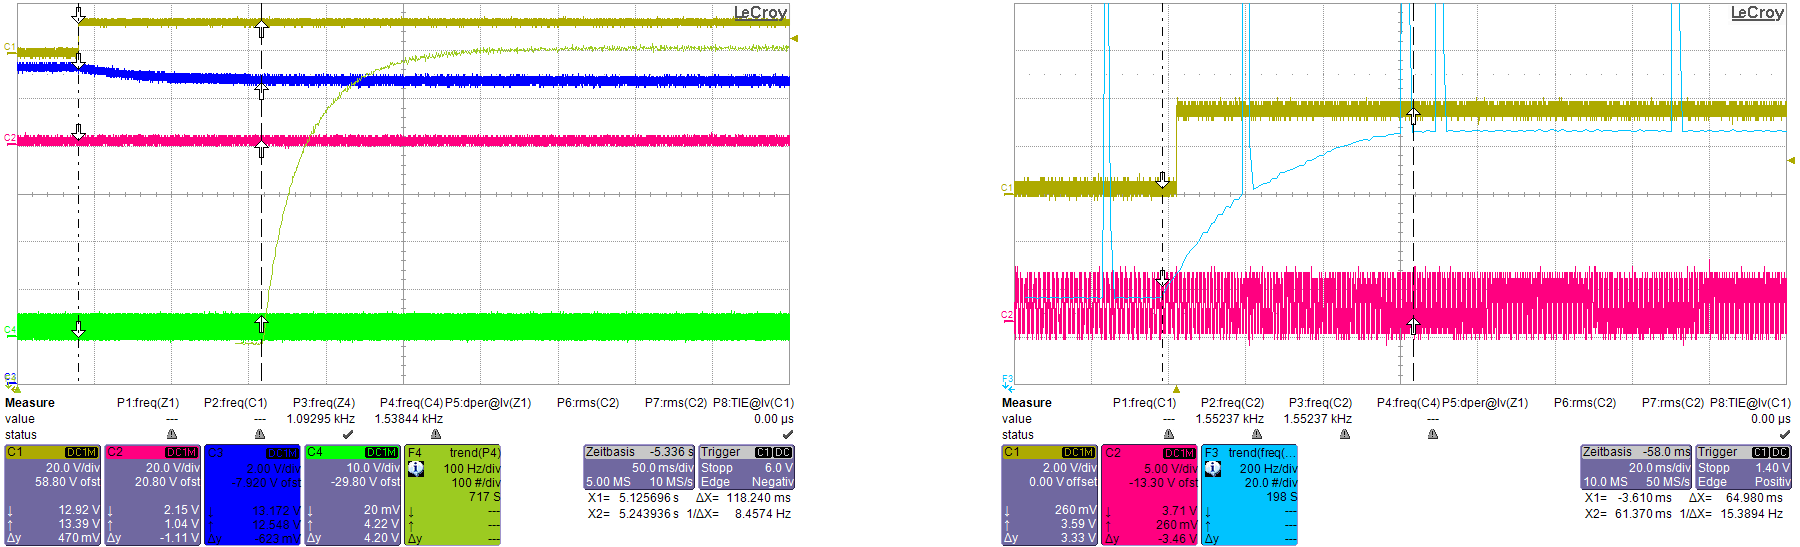
\includegraphics[width=\textwidth]{sweep/comp_upsweep.png}\\[1ex]
	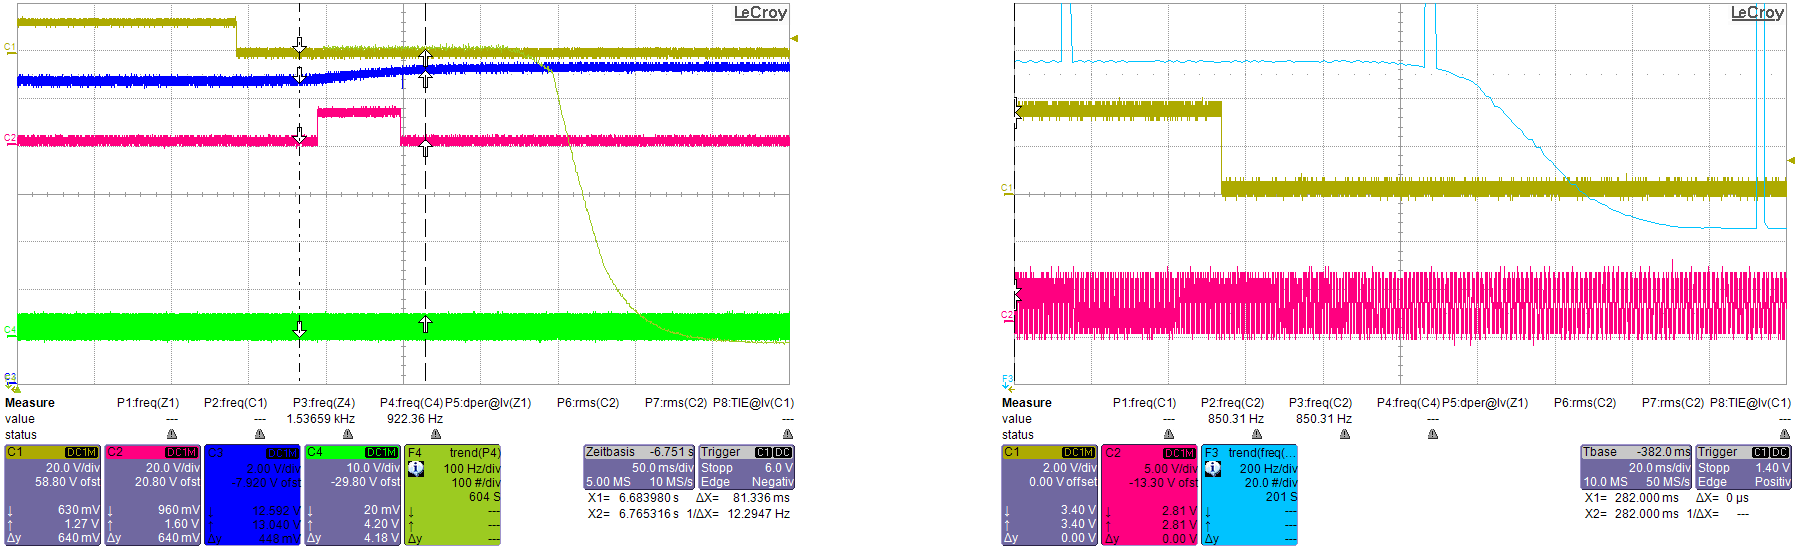
\includegraphics[width=\textwidth]{sweep/comp_downsweep.png}
	\caption[Frequency Sweep: Original Board and FPGA Emulation]{Frequency sweep of the original board (left capture of each pair) and of the \gls{fpga} emulation (right capture), recorded by Leyer on the inherited Rev~0.0 prototype in July~2023. Top: rising sweep; bottom: falling sweep. The thin lines are the oscilloscope's trends of the frequency measurement: they plot its successive values, 100 per division for the original board and 20 for the emulation, so their horizontal axis is not the time base of the traces, although Leyer describes them as the change of frequency over time~\cite[Sec.~4.10]{leyer2023}. The readouts are given in \Cref{tab:sweep_readouts}. Reproduced from~\cite[Figs.~11 and~12]{leyer2023}.}
	\label{fig:sweep_comparison}
\end{figure}

\Cref{tab:sweep_readouts} gives the readouts of the sweep captures. Leyer reports that the end frequencies of \SI{850}{\hertz} and \SI{1550}{\hertz} and the duration of the sweep were checked against the original board and showed the correct values, but gives no values~\cite[Sec.~4.10]{leyer2023}. Read from the captures, the frequency readouts of the original board are \SI{1538.44}{\hertz} in the rising and \SI{922.36}{\hertz} in the falling sweep, those of the emulation \SI{1552.37}{\hertz} and \SI{850.31}{\hertz}. For the self-test of the original test card, the fixture report gives a frequency change from \SI{1540}{\hertz} to \SI{920}{\hertz}~\cite[Sec.~5.1.5]{dolata2023}, in line with the original board's readouts, while the emulation's sweep is designed for \SIrange{849.9}{1549.6}{\hertz} (\Cref{eq:sweep}). The captures do not show what the readouts were measured over, and most of them carry a warning symbol of the oscilloscope. Further captures of the original board in the folder \texttt{Analyse} of Leyer's digital appendix~\cite{leyer2023}, however, read \SI{919.69}{\hertz} (\texttt{ss4.png}), \SI{920.81}{\hertz} (\texttt{ss9.png}) and \SI{920.80}{\hertz} and \SI{921.80}{\hertz} (\texttt{ss34.png}) at the low end. The raw export of the window of \texttt{ss34.png} (\path{C4Signal_red00000.csv}) shows a steady frequency: its 459 periods, evaluated for this report, lie between \SI{916}{\hertz} and \SI{926}{\hertz}, about \SI{920}{\hertz} on average. The periods were taken between consecutive rising crossings of the midpoint between the signal's extremes (\SI{2.12}{\volt}), at the resolution of one sample (\SI{4}{\micro\second}) and with a hysteresis of \SI{0.5}{\volt}. The low end of the original board is therefore about \SI{920}{\hertz}, about \SI{70}{\hertz} above that of the emulation. Leyer's analysis note in the same folder gives \SI{850}{\hertz} as the intended value (\texttt{Widerstände Sweep Counter.txt}); whether \SI{920}{\hertz} is the design value of the original circuit or a drift of this board is open. This report does not record whether Leyer's captures and the fixture report's values for the original test card come from the same unit; if they came from two units, a drift common to both would be less likely, but as it stands the agreement of the two values does not settle the question.

The duration differs as well, as far as the sources allow a comparison. The emulation's rising sweep reaches its end value after about \SI{52}{\milli\second} and its falling sweep after about \SI{102}{\milli\second} (\Cref{sec:fpga_core_details}); its falling table reaches about \SI{920}{\hertz} after 33 steps, about \SI{55}{\milli\second}. For the original test card, the fixture report gives about \SI{180}{\milli\second} for the frequency changes, which its capture reads with cursors as \SI{183.186}{\milli\second}~\cite[Sec.~5.2, Fig.~3]{dolata2023}. The cursor spacings of Leyer's captures (\Cref{tab:sweep_readouts}) cannot be set against these figures, for the reason given with \Cref{tab:sweep_readouts}. Because the sweep simulates a misbehaviour that the axle cards are to recognise as sliding~\cite[Sec.~2.9]{leyer2023}, its duration and slope may matter as much as its end frequencies; the sources do not say which of them the axle cards evaluate. Both points concern the original board rather than the emulation: the emulation's end frequencies and durations follow from its tables and clock dividers, so a measurement of the rebuilt unit would be expected to show these design values if its \gls{fpga} design contains this generator. Settling the low end and the duration of the original's sweep needs a re-measurement of the original board or a check of its sweep circuit; both are open (\Cref{tab:evidence_state}).

\begin{table}[htbp]
	\centering
	\caption[Readouts of the Sweep Captures]{Readouts of the sweep captures of \Cref{fig:sweep_comparison}, read from the archived images, not measured again. P2 to P4 are the measurement parameters as the oscilloscope labels them; what the cursors mark is not documented.}
	\label{tab:sweep_readouts}
	\small
	\begin{tabular}{@{}lll@{}}
		\toprule
		Readout & Original board (left) & \gls{fpga} emulation (right) \\
		\midrule
		Rising sweep: frequency of the channel & \SI{1538.44}{\hertz} (P4) & \SI{1552.37}{\hertz} (P2, P3) \\
		Rising sweep: frequency of the zoomed trace & \SI{1092.95}{\hertz} (P3) & -- \\
		Rising sweep: cursor spacing & \SI{118.240}{\milli\second} & \SI{64.980}{\milli\second} \\
		Falling sweep: frequency of the channel & \SI{922.36}{\hertz} (P4) & \SI{850.31}{\hertz} (P2, P3) \\
		Falling sweep: frequency of the zoomed trace & \SI{1536.59}{\hertz} (P3) & -- \\
		Falling sweep: cursor spacing & \SI{81.336}{\milli\second} & 0 (cursors coincide) \\
		Time base & \SI{50}{\milli\second}/div & \SI{20}{\milli\second}/div \\
		\bottomrule
	\end{tabular}
\end{table}

\subsection{Layer 2: System-Level Test Results}
\label{subsec:system_scenario_results}

In this method, fixture-based testing is the decisive check of functional equivalence. Before the rebuilt unit could be tested, the follow-on team had to make the fixture's firmware debuggable and correct its state machine~\cite[p.~10]{savchuk2025}. On the rebuilt unit the Layer~2 evidence is their report; no fixture log was archived:
\begin{itemize}
	\item \textbf{Fault Memory Cycle:} The legacy diagnosis table~\cite[Blatt~20/25]{rexroth1992wsp} lists, for each of the four axle cards, codes for a sensor fault, a valve short circuit, a valve wire break and a monitoring timeout, and codes for the computer cards 01 to 05. Before the rebuilt unit was tested, the follow-on team had revised the PC software of the fixture so that tests setting two or three pins at once could run~\cite[pp.~10--11]{savchuk2025}. After the \gls{nvram} enable defect (B1) had been corrected, the two-pin tests still aborted, which the team attributed to the PC software~\cite[p.~14]{savchuk2025}. The team then ran the fixture's full suite, which it reports as successful, and a selection of 19 test cases; the expected codes were observed on the displays, but the fixture's camera could not read them~\cite[p.~15]{savchuk2025}. The follow-on report does not say how the abort of the two-pin tests was resolved before these runs. No test log of these runs is part of the archived material. Which fault codes these runs covered is not recorded here. For the sensor faults, \enquote{expected} means the fixture's display code, 31 for axle card~3, where \Cref{tab:requirement_basis} gives 03 (note~b), so for these cases the observation cannot be read as conformity with that table.
	\item \textbf{Self-Test:} The execution of the legacy self-test on the rebuilt unit is not documented. Leyer's simulation showed the start of the self-test sequence as intended~\cite[Sec.~5.1.2]{leyer2023}. The fixture firmware used in the follow-on runs had gained a self-test function~\cite[p.~12]{savchuk2025}; the follow-on report says neither what it tests nor whether those runs used it.
	\item \textbf{User Interface Equivalence:} STW and Lösch are part of the fixture's test sequence~\cite{dolata2023}, and the Lösch function worked after the correction of B1~\cite[p.~14]{savchuk2025}; for the Test and Tür/V buttons no result on the rebuilt unit is documented.
	\item \textbf{Power-Cycle Stability:} No run with power cycles on the rebuilt unit is recorded.
	\item \textbf{\gls{stm32} Diagnostics Logging:} Both defects of the diagnostic path (B4, B5) were open in August 2025~\cite[pp.~19--22]{savchuk2025}; a fix of the firmware of 2023, described in \Cref{sec:diagnostic_resolution}, was applied afterwards; the evidence after it is given in \Cref{tab:evidence_state}.
\end{itemize}

\Cref{tab:results_summary} summarises the verification activities by layer, with the item tested, the date and the source of each result.

% p: with its notes the table is too tall for the top of a text page, and without p it
% held back every later table of the chapter until the chapter ended
\begin{table}[htbp]
	\centering
	\caption[Summary of Verification Results]{Summary of verification results across both layers, with the item tested, the date and the source of each result.}
	\label{tab:results_summary}
	\small
	\setlength{\tabcolsep}{4pt}
	\begin{tabular}{@{}>{\raggedright\arraybackslash}p{0.25\textwidth} l >{\raggedright\arraybackslash}p{0.2\textwidth} >{\raggedright\arraybackslash}p{0.09\textwidth} >{\raggedright\arraybackslash}p{0.13\textwidth} >{\raggedright\arraybackslash}p{0.16\textwidth}@{}}
		\toprule
		Test category & Layer & Item tested & Date & Source & Result \\
		\midrule
		Design simulation in ModelSim (boot, error storage) & L1 & Design of 2023 & 2023 & \cite[Sec.~5.1]{leyer2023} & Pass$^{a}$ \\
		Flash and \gls{nvram} test designs & L1 & Rev~0.0 prototype & 2023 & \cite[Sec.~4.3--4.4]{leyer2023} & Pass \\
		\gls{jtag} ID and programming & L1 & Rev~0.0 prototype & 2023 & \cite[Sec.~4.1]{leyer2023} & Pass \\
		Watchdog reaction & L1 & Rev~0.0 prototype & Aug.\ 2023 & \cite[Sec.~4.6]{leyer2023} & Observed$^{b}$ \\
		Watchdog reaction & L1 & Rebuilt unit, before re-soldering & 2025 & \cite[p.~13]{savchuk2025} & Before rework$^{b}$ \\
		Frequency sweep & L1 & Rev~0.0 prototype and original board & July 2023 & \cite[Sec.~4.10]{leyer2023} & Observed$^{b}$ \\
		Frequency sweep & L1 & Rebuilt unit & -- & -- & Not documented \\
		Fault codes & L2 & Rebuilt unit$^{f}$ & 2025 & \cite[p.~15]{savchuk2025} & Observed$^{c}$ \\
		Operator buttons STW, Lösch & L2 & Rebuilt unit$^{f}$ & 2025 & \cite[pp.~14--15]{savchuk2025} & Observed$^{c}$ \\
		Operator buttons Test, Tür/V & L2 & Rebuilt unit & -- & -- & Not documented \\
		Self-test & L2 & Rebuilt unit & -- & -- & Not documented \\
		Power-cycle stability & L2 & Rebuilt unit & -- & -- & Not documented \\
		Diagnostic \gls{spi} frame & L2 & Rebuilt unit$^{f}$ & -- & -- & Fix applied$^{d}$ \\
		\gls{sd}~card logging & L2 & Rebuilt unit$^{f}$ & -- & -- & Fix applied$^{e}$ \\
		\bottomrule
	\end{tabular}

	\medskip
	\begin{minipage}{0.95\textwidth}
		\footnotesize
		$^{a}$The archived simulation could not detect defect~B1, because its \gls{nvram} model ignores the byte-low enable (\Cref{subsec:fpga_interface_results}).\\
		$^{b}$The archived oscilloscope captures (\Cref{fig:watchdog_reaction,fig:sweep_comparison}) were taken by Leyer on the inherited Rev~0.0 prototype, the sweep also on the original board; the readouts of the sweep are given in \Cref{tab:sweep_readouts}. The cursor readout in~\Cref{fig:watchdog_reaction} measures no watchdog parameter; the timing read from the capture, and Leyer's doubts about it, are given in \Cref{subsec:fpga_interface_results}; unlike the sweep, the watchdog has no capture of the original board as a reference~\cite[Sec.~4.6]{leyer2023}. On the rebuilt unit, the follow-on report's only statement on the watchdog refers to the state before the re-soldering of the \gls{fpga} pins (\Cref{subsec:fpga_interface_results}).\\
		$^{c}$Observed during the follow-on runs (full suite and 19 selected cases); the fixture's camera could not read the displays (\Cref{tab:evidence_state}).\\
		$^{d}$Truncated to 16~bits in the inherited firmware; in 2025 the third byte was also found corrupted in simulation (defect~B5). A fix was applied to the receiver of 2023; whether the transmitter was changed is not documented.\\
		$^{e}$The logging froze with the follow-on firmware of 2025; frames were overrun in the firmware of 2023, to which a fix was applied (defect~B4). For the evidence after the fix of this row and the row above, see \Cref{tab:evidence_state}.\\
		$^{f}$Configuration not documented: the follow-on report names the~\gls{fpga} design of the rebuilt unit only as the new software of the test card, without a version or checksum, and does not say which firmware ran on its \gls{stm32} Diagnostics Board~\cite[p.~15]{savchuk2025} (\Cref{sec:diagnostic_resolution}).
	\end{minipage}
\end{table}

\subsection{State of the Evidence}
\label{subsec:equivalence_discussion}

The central question of whether functional equivalence has been demonstrated cannot yet be answered in the affirmative: simulation and the fixture runs indicate equivalence of the fault handling, the captures of the original board point to a deviation of the sweep, two hardware changes alter the behaviour of the module by design (\Cref{sec:en50716_modifications}), and the evidence is incomplete. \Cref{tab:evidence_state} lists what the evidence consists of, when it was produced and whether it was kept, and so collects its gaps in one place.

% p: with the row of the missing tolerances the table no longer fits below the text of
% its page, and without p it held back every later table of the chapter until its end
\begin{table}[htbp]
	\centering
	\caption[State of the Evidence]{State of the evidence for functional equivalence. \enquote{Kept} means kept with the project's files; none of these files is published with this report.}
	\label{tab:evidence_state}
	\small
	\begin{tabular}{@{}>{\raggedright\arraybackslash}p{0.31\textwidth} >{\raggedright\arraybackslash}p{0.11\textwidth} >{\raggedright\arraybackslash}p{0.38\textwidth} >{\raggedright\arraybackslash}p{0.11\textwidth}@{}}
		\toprule
		Object & Date & Evidence & Kept \\
		\midrule
		Design of 2023: simulation of the complete design and of test designs & 2023 & Testbenches without assertions, results checked by eye~\cite[Sec.~5.1]{leyer2023}; B1 not visible to the testbench & Yes \\
		Rev~0.0 prototype: \gls{jtag}, pin, Flash, \gls{nvram}, I/O, \gls{bod}, display and button tests & 2023 & Test descriptions and protocols~\cite[Sec.~4.1--4.9, App.~A]{leyer2023} & Yes \\
		Rev~0.0 prototype and original board: frequency sweep & July 2023 & Oscilloscope captures (\Cref{fig:sweep_comparison}); low end differs from the original, open (\Cref{subsec:fpga_interface_results}) & Yes \\
		Original test card: duration of the sweep & 2023 & Capture in the fixture report~\cite[Sec.~5.2, Fig.~3]{dolata2023}, set against the emulation's design values (\Cref{sec:fpga_core_details}); duration differs, open (\Cref{subsec:fpga_interface_results}) & Report only \\
		Rev~0.0 prototype: watchdog reset & Aug.\ 2023 & Oscilloscope capture (\Cref{fig:watchdog_reaction}); no reference from the original board & Yes \\
		Rebuilt unit: commissioning and debugging (B1, B3, B6) & 2025 & Follow-on report~\cite[pp.~13--14]{savchuk2025} & Report only \\
		Rebuilt unit: fixture suite and 19 selected cases & 2025 & Follow-on report~\cite[p.~15]{savchuk2025}; the codes covered are not recorded & Report only, no log \\
		Logger of 2025: simulation (B5) & 2025 & Follow-on report~\cite[p.~21]{savchuk2025} & Report only \\
		Rebuilt unit after the fix of B4 and B5: operation as a whole in the test setup & Early 2026 & Observed by the author, the supervisor and members of the project team; diagnostic path not verified separately & No log or capture \\
		Rebuilt unit: self-test, Test and Tür/V buttons, power cycles, watchdog, sweep, \gls{bod} & -- & None documented & -- \\
		Design of 2023: STORE and RECALL inputs (08z, 08d), added \gls{bod} circuit & 2023 & Deviations by design (\Cref{sec:en50716_modifications}): the inputs no longer act on the fault memory, and the \gls{bod} circuit adds a reset; their relevance in the vehicle is open & Yes \\
		Acceptance criteria: tolerances for the sweep, the display rhythm and the self-test duration & -- & None defined; nominal values only (\Cref{subsec:requirement_basis}) & -- \\
		\bottomrule
	\end{tabular}
\end{table}

The three lines of evidence, simulation, hardware measurement and system tests, observe different aspects of correctness (logical, physical, behavioural), but not the same object: the first two concern the design and the Rev~0.0 prototype of 2023, before the rebuild, and only the third concerns the rebuilt unit. They are also of unequal strength. The archived simulation could not detect B1, and no simulation after its correction is archived; the measurements were made on the prototype, the sweep against the original board; and the system tests on the rebuilt unit are known only from the follow-on report. Simulation and the fixture runs indicate equivalence of the fault handling. The sweep, however, deviates from that of the original board, and this point is open: at its low end in Leyer's comparison captures, and in its duration when the emulation's design values (\Cref{sec:fpga_core_details}) are set against the fixture report's capture of the original card~\cite[Sec.~5.2, Fig.~3]{dolata2023} (\Cref{subsec:fpga_interface_results}). Two further deviations follow from the design (\Cref{sec:en50716_modifications}): the STORE and RECALL inputs of the system connector (08z, 08d) no longer act on the fault memory, and the added \gls{bod} circuit holds the emulated controller in reset when a sensed supply voltage falls below its threshold (\Cref{sec:redundancy_failsafe}). Whether the vehicle drives these inputs is open, and so is whether a reset in service leads into the automatic check (\Cref{sec:vehicle_outputs}). The evidence therefore does not demonstrate equivalence: a logged repetition of the Layer~2 suite and of the Layer~1 measurements on the rebuilt unit would close the gap for that unit, and a re-measurement of the original board's sweep or a check of its sweep circuit would settle the deviation (\Cref{sec:future_work}).

Some limits of the evidence cannot be removed within this report. The design and test sources are not published with it (\Cref{sec:fpga_core_details}). The evidence for the rebuilt unit rests on an unpublished project report~\cite[pp.~13--15]{savchuk2025} and on runs and an observation whose data were not kept. Whether the layouts pass a design-rule check run today is unknown (\Cref{sec:app_drc}). There is no test specification: the expected codes of the fixture's test cases are the only pass/fail criteria (\Cref{chap:safety_checklist}, item~CL-A6). The verification layers are mapped to whole standards, not to individual clauses (\Cref{tab:standards_mapping}).

Because the method relies on generic V-model principles and on black-box behaviour at the board's inputs and outputs rather than on knowledge specific to this system, it can in principle be transferred to other hardware retrofits under \gls{iec61508}, although only this one case has been examined so far.

% ------------------------------------------------------------
\section{Integration Defects and Where They Surfaced}
\label{sec:integration_defects}

Six defects documented during the rebuild of the unit are classified in \Cref{tab:bug_taxonomy} by type and by how they were found. B1 to B3, B6, the freeze of B4 and the transmitter part of B5 are documented in the follow-on report~\cite[pp.~10--21]{savchuk2025}; the overrun of B4 and the 16-bit reception of B5 are described in the Working Paper~\cite[Sec.~V-E]{torun2026}. The defects did not come to light in a planned run of the two-layer method.

% p: with the separated entries of B4 and B5 the table no longer fits below the text of
% its page, and without p it held back every later table of the chapter until its end
\begin{table}[htbp]
	\centering
	\caption[Classification of the Discovered Integration Defects]{Classification of the discovered integration defects.}
	\label{tab:bug_taxonomy}
	\small
	\begin{tabular}{@{}l l >{\raggedright\arraybackslash}p{0.3\textwidth} >{\raggedright\arraybackslash}p{0.19\textwidth} >{\raggedright\arraybackslash}p{0.19\textwidth}@{}}
		\toprule
		ID & Class        & Description                                                                       & Found by                                                  & Status               \\
		\midrule
		B1 & Logical      & \gls{nvram} byte-low enable (\texttt{NVRAM\_ble}) held high                       & Symptoms on the fixture (L2), cause by debugging          & Resolved             \\
		B2 & Test fixture & SWD pins of the fixture's \gls{stm32} assigned to general-purpose I/O              & Failed debugger connection to the fixture                 & Reworked             \\
		B3 & Assembly     & Four and then about 40 further \gls{fpga} pins poorly soldered                     & Commissioning; how the faults were noticed is not recorded (oscilloscope: supply and clock present) & Reworked             \\
		B4 & Firmware     & \gls{sd}-card logging froze with the follow-on firmware of 2025, cause not established, no fix of that firmware documented~\cite[pp.~16--19, 22]{savchuk2025}; frames overrun by the mount overhead of the firmware of 2023, to which the fix was applied & Freeze: operation of the \gls{stm32} Diagnostics Board (2025); overrun: analysis of the firmware of 2023 & Fix applied (firmware of 2023); diagnostic path not verified separately$^{a}$; freeze with the firmware of 2025: no fix documented \\
		B5 & Interface    & \gls{spi} frame truncated to 16 of 32~bits (firmware of 2023); third byte corrupted by the \gls{vhdl} transmitter (2025); polarity and slave select at the receiver open (\Cref{sec:diagnostic_resolution}) & Transmitter: simulation testbench (L1); receiver: not recorded & Receiver: fix applied; transmitter: change not documented; diagnostic path not verified separately$^{a}$ \\
		B6 & \begin{tabular}[t]{@{}l@{}}Schematic\\and layout\end{tabular} & LED Board Rev~1.0 (2024): driver-to-display assignment reversed against the design of 2023, \texttt{Y13} (left digit) drives \texttt{DS2} and \texttt{Y14} (right digit) \texttt{DS1}$^{b}$ & Commissioning of the rebuilt unit~\cite[p.~13]{savchuk2025} & Worked around in the \gls{fpga} design (\texttt{atop.vhd}), not on the LED Board~\cite[p.~13]{savchuk2025} \\
		\bottomrule
	\end{tabular}

	\medskip
	\begin{minipage}{0.9\textwidth}
		\footnotesize
		$^{a}$The diagnostic path comprises the \gls{sd}-card logging and the complete \gls{spi} frames; for the observation of early 2026 see \Cref{sec:diagnostic_resolution} and \Cref{tab:evidence_state}.\\
		$^{b}$The reversal entered with the Rev~1.0 files of June 2024, in which the displays were replaced (\Cref{app:schematics}); in every design file of 2023, \texttt{Y13} drives the display at the position of \texttt{DS1}. The corrected \texttt{atop.vhd} is not archived, and the workaround belongs together with this LED Board.\\
		Who did what: B1 and B2 were found and corrected, and B6 was found and worked around, by the follow-on team~\cite[pp.~10--14]{savchuk2025}. Of the poorly soldered pins (B3), the first four were re-soldered by the supervisor; who re-soldered the about 40 further pins is not stated~\cite[p.~13]{savchuk2025}. The follow-on team documented the freeze of B4 and the transmitter part of B5~\cite[pp.~19, 21]{savchuk2025}. The overrun of B4 and the 16-bit reception of B5 are described in the Working Paper~\cite[Sec.~V-E]{torun2026}; who found them, and who applied the fix of B4 and B5, is not recorded.
	\end{minipage}
\end{table}

An analysis of these defects shows why the two layers are complementary, and also where the evidence ends. The structure does not introduce a new testing paradigm; it applies the V-model principle of structural component tests followed by functional system validation to a hardware and firmware retrofit.

No single method found all six defects. The archived simulation of 2023 could not detect B1, because the testbench's model of the \gls{nvram} ignores the byte-low enable (\Cref{subsec:fpga_interface_results}); its symptoms appeared at the board boundary when the rebuilt unit was tested on the fixture, and its cause was located by debugging. The solder defects (B3) surfaced during commissioning, when the processor did not start although supply and clock were present. The swapped displays (B6), which come from the driver-to-display assignment of the Rev~1.0 LED Board, were noticed once the rebuilt unit could be switched on. B2 lay in the test equipment rather than in the device under test. Of the diagnostic-path defects, the corruption of the third byte (B5) was found in a simulation testbench, while the freeze of the \gls{sd}-card logging (B4) appeared only when the \gls{stm32} Diagnostics Board ran with its firmware.

The defects therefore support a weaker statement than a proof of the method: component-level simulation and system-level testing each saw some defects and missed others, and the solder defects surfaced only during commissioning. They illustrate the need for several complementary verification methods; they do not show that the two layers together detect all defects of this kind.

% ------------------------------------------------------------
\section{Causes of the Diagnostic-Path Defects and the Fix Applied}
\label{sec:diagnostic_resolution}

The two defects of the diagnostic path lie in the interplay of the \gls{fpga}, the isolated link and the \gls{stm32} firmware. Their causes and the fix applied are described below:
\begin{description}
	\item[SD Card Storage (B4):] The follow-on team found that the \gls{sd}-card logging froze when the \gls{stm32} Diagnostics Board ran the team's own firmware~\cite[pp.~19, 22]{savchuk2025}, which reads the frames bit by bit by polling the pins and mounts and unmounts the file system for every write~\cite[pp.~16--18]{savchuk2025}. The sources do not establish the cause of this freeze. An analysis of the inherited firmware of 2023 (\texttt{USB\_RTC\_SD\_Test}) found a fault in the same path: it mounted and unmounted the file system volume around every write in the logging loop, which added a blocking overhead that was not measured, and its main loop contained two further blocking delays of \SI{500}{\milli\second} each. Together these delayed the re-arming of the \gls{spi} receive interrupt, so that frames were overrun, and an overrun loses the bytes that follow~\cite[Sec.~20.3.10]{st_rm0368}. The firmware re-arms the reception (\path{HAL_SPI_Receive_IT}) only after a completed one (\texttt{main.c}, lines 125, 166 and 455--457) and defines no error callback, and the archived driver \path{stm32f4xx_hal_spi.c} aborts an interrupt reception when an overrun is pending (\path{HAL_SPI_IRQHandler}); according to the code, no further frame is received after an overrun, while the periodic log entries of the main loop continue. The fix applied to the firmware of 2023 mounts the card once at initialisation, removes the mount calls from the loop and reduces the logging frequency; whether it would also remove the freeze observed with the firmware of 2025 is not established, and no fix of that firmware is documented~\cite[pp.~16--19, 22]{savchuk2025}.
	\item[SPI Payload Truncation and Alignment (B5):] The \gls{vhdl} \gls{spi} master of 2023 transmits a 32-bit diagnostic frame (\Cref{sec:fpga_core_details}): a 2-bit event-type prefix, the six button states and the 24-bit error vector. The inherited \gls{stm32} firmware, however, was the test program of Leyer's link test (\texttt{USB\_RTC\_SD\_Test}, \Cref{sec:stm32_details}), because no code to interpret these frames existed yet~\cite[Sec.~3.3]{leyer2023}; it received only 16~bits per transaction: \texttt{HAL\_SPI\_Receive\_IT} was called with a buffer of two elements at an 8-bit data size. The remaining 16 clock cycles of each frame left data unread and set the receiver overrun flag (\texttt{OVR} in the \gls{spi} status register~\cite[Sec.~20.3.10]{st_rm0368}); the Working Paper speaks of misaligned subsequent frames~\cite[Sec.~V-E]{torun2026}, whereas according to the archived code the reception ends at that overrun (B4 above). For the 16-bit reception of the firmware of 2023, the fix sizes the reception to the full frame, four bytes at the 8-bit data size, which removes the truncation. In August 2025 the follow-on project documented a second cause in the \gls{fpga}: in the simulation of its logger, the first two bytes of each frame were transferred correctly and the third byte was corrupted; the transmitter had not yet been tested on the hardware~\cite[p.~21]{savchuk2025}. Two further facts of the design bear on the alignment and are open points; they are described at the end of this section.
\end{description}

The description of these causes and fixes follows the Working Paper~\cite[Sec.~V-E]{torun2026}; the causes can be checked against the archived firmware of 2023, while the changed firmware is not archived. Both fixes concern the firmware of 2023 (\texttt{USB\_RTC\_SD\_Test}) and the 32-bit logger of 2023 that it receives from; they do not concern the follow-on project's three-byte logger or its own firmware, which reads the three bytes bit by bit and also mounts the card for every write~\cite[pp.~16--17]{savchuk2025}. Which logger the \gls{fpga} design of the rebuilt unit contains, and which firmware runs on its \gls{stm32} Diagnostics Board, is not documented.

Both defects were open when the follow-on project reported in August 2025~\cite[pp.~19, 21]{savchuk2025}: the SD-card logging froze, and in simulation the VHDL transmitter corrupted the third byte of each frame. A fix of the STM32 firmware of 2023 was applied afterwards; whether the VHDL transmitter was changed after the finding of 2025 is not documented. In early 2026 the author, the supervisor and members of the project team observed the rebuilt unit operating as a whole in the test setup; the diagnostic path itself was not verified separately, and no log or capture of that run was archived.

Both defects concern the non-safety-related diagnostic function. B4 and the receiver part of B5 lie in the \gls{stm32} Diagnostics Board, which is galvanically isolated from the \gls{fpga} core (\Cref{sec:stm32_details}); the transmitter part of B5 lies in the logger module of the \gls{fpga} design. The four optocouplers carry signals only from the Base Board to the \gls{stm32} Diagnostics Board, and the isolated side has its own power domain, so by design faults on the isolated side cannot feed back into the \gls{fpga} domain through the signal path, as long as the solder jumper \texttt{SJ2}, which can bridge the two grounds, stays open (\Cref{tab:bom}). This does not cover the parts of the \gls{stm32} Diagnostics Board on the Base Board side of the barrier, which remain a fault path into the Base Board, and no test of the isolation is documented (\Cref{sec:stm32_details}).

\subsubsection{Polarity and Slave Select of the SPI Link}

The optocoupler stages \texttt{OK5}, \texttt{OK6} and \texttt{OK8} are common-emitter stages with collector pull-ups (\texttt{R108}--\texttt{R110}), so the \gls{stm32} receives each \gls{spi} line inverted (\Cref{fig:schematic_sheet4}). The \gls{spi} core of 2023 idles the slave select high and the clock low, and \texttt{atop.vhd} passes both through uninverted, so that at the \gls{stm32} the slave select is active and the clock high while the link is idle, and the data arrive inverted. The firmware of 2023 also takes its hardware slave select from the pin \texttt{PA15}, which the board leaves unconnected; the schematic routes the slave select to \texttt{PA4} (net \texttt{MCU\_SPI\_!SS}), in Rev~0.0 as in Rev~1.0. A buffer of four bytes makes the receiver take a whole frame per call, but it does not mark where a frame begins, which is the task of the slave select~\cite[Sec.~20.3.1]{st_rm0368}; without it, the alignment holds only as long as no clock edge is lost or added. Leyer's link test on the Rev~0.0 prototype~\cite[Sec.~4.11.2]{leyer2023}, which has the same stages and routing, used 8-bit test codes, \texttt{00000001} to \texttt{00000100} in \path{SPI_STM_top.vhd} of the archived test design \path{SPI_Test_STM32_final}; his documentation does not say how the inversion was handled there. What the applied fix did about the polarity and the slave select is not documented.

% ------------------------------------------------------------
\section{Relation to Safety Standards}
\label{sec:safety_compliance}

The project's methodology and artefacts were developed to support a future safety certification process. \Cref{tab:standards_mapping} summarises how the methodology maps to the applicable standards. In this report, a standard is \emph{mapped} to the verification layers whose activities bear on the aspect named in its row: the mapping is made for whole standards, not for individual clauses, and it is not an assessment of compliance; the table names only the parts, annexes and scope statements of each standard on which the text relies. For~\gls{en50155} and~\gls{en61373} it names future work only. The mapping to five standards stated in the abstract is meant in this sense. No integrity level in the sense of~\gls{ieee1012}, which specifies its~\gls{vv} requirements for different integrity levels~\cite{ieee1012_2024}, and no~\gls{sil} have been assigned, because no hazard analysis has been made that could support either (\Cref{chap:safety_checklist}, item~CL-A4).

\begin{table}[htbp]
	\centering
	\caption[Mapping of the Verification Layers to the Standards]{Mapping of the verification layers to whole standards, with the parts of each standard on which the text relies; the mapping is not an assessment of compliance.}
	\label{tab:standards_mapping}
	\small
	\begin{tabular}{@{}>{\raggedright\arraybackslash}p{0.16\textwidth} >{\raggedright\arraybackslash}p{0.27\textwidth} >{\raggedright\arraybackslash}p{0.39\textwidth} l@{}}
		\toprule
		Standard & Scope & Parts the text relies on & Layer \\
		\midrule
		\gls{iec61508}~\cite{iec61508_2010} & Verification in the safety lifecycle; no \gls{sil} assigned & Part~2: design and manufacture of the system except software~\cite{iec61508_2_2010}, here the \gls{fpga} implementation (\Cref{sec:standards_detail}); Part~3: software of safety-related systems (\Cref{sec:fpga_core_details}) and support tools~\cite{iec61508_3_2010} & L1 + L2 \\
		\gls{en50129}~\cite{en50129_2018} & Hardware safety evidence & Scope: modification of systems accepted before it, as far as reasonably practicable; informative Annex~F: user-programmable integrated circuits~\cite{en50129_2018} & L1 + L2 \\
		\gls{en50716}~\cite{en50716_2023} & Software aspects of the modification & Scope: software and its interaction with the system to which it belongs~\cite{en50716_2023} & L1 + L2 \\
		\gls{en50155}~\cite{en50155_2021} & Electronic equipment of rolling stock & -- & Future \\
		\gls{en61373}~\cite{en61373_2010} & Shock and vibration & -- & Future \\
		\gls{ieee1012}~\cite{ieee1012_2024} & \gls{vv} process; no integrity level assigned & Scope: \gls{vv} processes for different integrity levels~\cite{ieee1012_2024} & L1 + L2 \\
		\bottomrule
	\end{tabular}

	\medskip
	\begin{minipage}{0.95\textwidth}
		\footnotesize
		A mapping clause by clause needs the full texts of the standards, which this edition did not have; the third column names only parts, annexes and scope statements that the text uses and that the cited descriptions of the standards state, and no clause number.
	\end{minipage}
\end{table}

\begin{description}
	\item[Lifecycle Model:] The two layers are mapped to the verification side of the V-model (\Cref{fig:v_model_mapping}); its other side, from a requirements specification down to the design, is not documented in this report (\Cref{subsec:v_model_mapping}). The iterative debugging and the documentation of the fixes provide part of the audit trail that change management needs; that trail is incomplete (\Cref{sec:diagnostic_resolution}, \Cref{tab:evidence_state}).
	\item[Evidence for Verification Objectives:] The generated artefacts (\Cref{sec:verification_artefacts}) provide the evidence for~\gls{vv}, with the gaps named there. The debug report of the follow-on work~\cite[pp.~10--15]{savchuk2025} documents the anomalies found and how they were handled.
	\item[Traceability:] No requirement list exists. The Layer~1 tests were derived from the functions identified by reverse engineering and have no documented requirement to trace to; the Layer~2 YAML scenarios are linked to the fault cases of the legacy diagnosis table~\cite{rexroth1992wsp} by name, without the self-test (\Cref{sec:verification_artefacts}). The archived artefacts form part of the evidence base for a formal safety assessment; the Layer~2 test definitions and logs are not among them. For certification, requirements would have to be specified and linked to the tests in explicit matrices; the checklist in~\Cref{chap:safety_checklist} is a step towards this.
\end{description}

\subsection{The Two Layers and the V-Model}
\label{subsec:v_model_mapping}

As illustrated in \Cref{fig:v_model_mapping}, the two layers of the verification strategy are mapped to the right side of the V-model (\Cref{sec:derivation_of_strategy}), its verification and validation phases. Its left side would start from a requirements specification, which this report does not contain; the legacy behaviour serves as the requirement in its place (\Cref{chap:safety_checklist}, item~CL-A1).

\begin{figure}[htbp]
	\centering
	% V-model mapping of the two-layer verification strategy.
% Kept as diagram source rather than a bitmap so that it diffs, reviews and
% rebuilds deterministically with the rest of the document. The labels were
% German in earlier editions and are given in English here. Dashed arrows
% join a design level to the test level that checks it; at the bottom level
% the dashed arrow runs beside the solid one that continues the V.
\begin{tikzpicture}[
    x=1mm, y=-1mm,
    phase/.style={
      draw, fill=black!5,
      text width=42mm, align=center,
      inner sep=1.6mm, font=\small\bfseries,
      execute at begin node={\hyphenpenalty=10000 },
    },
    stage/.style={
      draw, text width=42mm, align=center,
      inner sep=1.6mm, minimum height=14mm, font=\footnotesize,
      execute at begin node={\hyphenpenalty=10000 },
    },
    flow/.style={-{Latex[length=2mm,width=1.6mm]}, thick},
    corr/.style={-{Latex[length=2mm,width=1.6mm]}, thick, densely dashed},
  ]

  \node[phase] (specphase) at (24, 6) {Design \& Specification};
  \node[phase] (vvphase)   at (118, 6) {Verification~\& Validation};

  \node[stage] (req)  at (24, 34) {\textbf{System Requirements}\\(legacy behaviour according to the original manual)};
  \node[stage] (arch) at (36, 62) {\textbf{Architecture Design}\\(FPGA/STM32 separation, module structure)};
  \node[stage] (mod)  at (48, 90) {\textbf{Module \& Component Design}\\(VHDL logic, schematics)};

  \node[stage] (unit)  at (106, 90) {\textbf{Unit \& Module Tests}\\\textbf{(Layer 1)}\\(VHDL simulation)};
  \node[stage] (integ) at (118, 62) {\textbf{Integration Tests}\\\textbf{(Layer 1)}\\(hardware measurements, interfaces)};
  \node[stage] (sys)   at (130, 34) {\textbf{System Validation}\\\textbf{(Layer 2)}\\(fixture tests, scenarios)};

  \draw[flow] (req)   -- (arch);
  \draw[flow] (arch)  -- (mod);
  \draw[flow] ([yshift=-3.5mm]mod.east) -- ([yshift=-3.5mm]unit.west);
  \draw[flow] (unit)  -- (integ);
  \draw[flow] (integ) -- (sys);
  \draw[corr] (req)   -- (sys);
  \draw[corr] (arch)  -- (integ);
  \draw[corr] ([yshift=3.5mm]mod.east) -- ([yshift=3.5mm]unit.west);

\end{tikzpicture}

	\caption[Mapping of the Test Strategy to the V-Model]{Mapping the two-layer test strategy to the verification and validation phases of the V-model. Solid arrows give the order of the phases; dashed arrows join a design level to the test level that checks it. It shows the mapping that Fig.~2 of the Working Paper~\cite{torun2026} shows, in a drawing of its own.}
	\label{fig:v_model_mapping}
\end{figure}

The Layer~1 tests (unit and integration tests) are meant to verify the correct implementation of the individual design modules at the code and hardware level, and the Layer~2 tests (system validation) to validate the fully integrated system against the original functional requirements. This structure is meant to support traceability and to provide, for each phase of the development lifecycle, the evidence that the standards require. Prior work by Ayoub and Leyer implicitly followed this principle; this report states the process explicitly as two layers (\Cref{chap:testing}), but it does not formalise it: no requirement list exists, and the Layer~2 cases are linked to the legacy faults only by name (\Cref{sec:verification_artefacts}).

This report describes how a~\gls{vv} evidence base for a retrofit can be built and so provides a starting point for a formal safety assessment; the gaps in this project's own evidence are named in~\Cref{subsec:limitations}. To the first research question (\Cref{sec:research_questions}) it gives a proposal rather than a demonstrated answer: a programme of two layers, component-level checks and measurements (Layer~1) and scripted system tests on a fixture (Layer~2), which observe different aspects of correctness (\Cref{chap:testing}). In this case the programme has not demonstrated functional equivalence: the evidence indicates equivalence of the fault handling but is incomplete, and the sweep deviates from the captures of the original board (\Cref{subsec:equivalence_discussion}). Whether the programme complies with current functional safety standards has not been assessed: its layers are only mapped to whole standards (\Cref{tab:standards_mapping}). It answers the second research question only in part: it proposes a verification framework and names the artefacts it produces (\Cref{sec:verification_artefacts,chap:safety_checklist}), but it defines no metrics, does not examine the cost of achieving and maintaining certification, and rests on a single case.

% ------------------------------------------------------------
\section{Discussion, Risk Management, and Limitations}
\label{sec:results_discussion_risk}

\subsection{Interpretation and Risk Management}
The verification outcomes indicate, but do not yet demonstrate, the viability of the \gls{fpga}-based retrofit approach (\Cref{subsec:equivalence_discussion}). The project addressed the following technical risks; no risk analysis was made (\Cref{chap:safety_checklist}, item~CL-A4):
\begin{itemize}
	\item \textit{Hardware Malfunction:} Risks from hangs or power anomalies are addressed by the hardware watchdog, tested on the prototype~\cite[Sec.~4.6]{leyer2023} (\Cref{fig:watchdog_reaction}), and by the \gls{bod} circuit, tested there too~\cite[Sec.~4.7]{leyer2023}, whose trip point on the core rail lies below the specified core supply (\Cref{sec:redundancy_failsafe}). On the rebuilt unit, no test of the \gls{bod} circuit is documented, nor any observation of the watchdog after the re-soldering of the \gls{fpga} pins (\Cref{subsec:fpga_interface_results}). The poor soldering of the \gls{fpga} pins was found during commissioning; after the re-soldering the unit could be switched on, and no inspection after the rework is documented~\cite[p.~13]{savchuk2025} (\Cref{chap:safety_checklist}, item~CL-B5).
	\item \textit{Diagnostic Interference:} The galvanic isolation of the \gls{stm32} subsystem is provided by design (optocouplers, isolated supply); it has not been tested separately. It is intended to keep faults on the isolated side out of the safety-related domain (with \texttt{SJ2} open); the parts of the \gls{stm32} Diagnostics Board on the Base Board side of the barrier remain a fault path into the Base Board supply (\Cref{sec:stm32_details}).
	\item \textit{Functional Deviation:} This primary risk was addressed through the testing and debugging cycle, which brought the rebuilt unit closer to the legacy behaviour; the evidence for that unit is incomplete, and the emulation's sweep deviates from the captures of the original board, an open point (\Cref{subsec:equivalence_discussion}).
\end{itemize}

\subsection{Limitations}
\label{subsec:limitations}
A continuation project inherits limitations as well as results, and naming them is part of the evidence:
\begin{itemize}
	\item \textbf{Residual Scope Gaps:} Formal methods (e.g., model checking or equivalence checking~\cite{formal_verification_rail_2023, mneimneh2005sequential}), quantitative structural coverage metrics (statement and branch coverage for the \gls{vhdl}), accredited environmental testing (\gls{en50155}~\cite{en50155_2021}, \gls{en61373}~\cite{en61373_2010}) and full \gls{hil} integration with the complete braking system were beyond the project's scope; they are identified as future work (\Cref{sec:future_work}). Which formal methods and coverage metrics a formal safety certification would expect depends on the \gls{sil} to be assigned, and none has been assigned (\Cref{sec:safety_compliance}); \gls{iec61508} grades its techniques and measures against the safety integrity level in Part~2 and against the required systematic capability in Part~3~\cite{iec61508_2_2010, iec61508_3_2010}.
	\item \textbf{Archived Evidence:} The gaps of the evidence are listed in \Cref{tab:evidence_state}. A certification campaign would have to carry out the missing measurements and runs on production hardware and archive them.
	\item \textbf{Diagnostic Path Robustness:} The fix for B4 mounts the volume once and reduces the logging frequency. The logging still runs in the main loop, so a non-blocking queue would remove the remaining dependence on the logging rate.
	\item \textbf{Long-Term Reliability:} While the rebuilt unit was observed operating as a whole after significant rework (\Cref{tab:evidence_state}), its long-term reliability is unproven. The follow-on team also observed an intermittent contact at both displays whose cause was not found; it may recur~\cite[p.~13]{savchuk2025}. The reliance on manual soldering for critical high-pin-count components is not suitable for a production environment. A new batch of professionally manufactured and assembled boards would be required for any deployment or accredited environmental testing.
\end{itemize}

\subsection{Economic and Sustainability Aspects}
The board-level retrofit is meant to let the existing system enclosure and main connectors be reused and to extend the life of the overall system. Its economic and ecological case is the general one for refurbishment set out in \Cref{sec:context} (\Cref{subsec:operational_economic_drivers}): refurbishment can defer capital expenditure and avoid the embodied emissions of manufacturing new subsystems. This report quantifies neither costs nor emissions, for the retrofit or for a full system replacement; an advantage over a replacement is therefore argued here, not shown.

% ============================================================
% Chapter 6: Conclusion and Future Outlook
% ============================================================
\chapter{Conclusion and Future Outlook}
\label{chap:conclusion}

This research addressed the challenge of modernising a legacy, safety-critical anti-skid test-diagnosis module. The project indicates, but does not yet demonstrate, that replacing an obsolete~\gls{mcs48}-based controller with a modern~\gls{fpga} (\texttt{Actel~A3P1000}) for logic emulation and an~\gls{stm32} microcontroller (\texttt{STM32F401RET6}) for enhanced diagnostics is a viable strategy. What the report contributes is a documented case, a classification of the six defects documented during the rebuild, and a proposed two-layer verification structure that has not been validated: the defects did not come to light in a planned run of it, and they illustrate why complementary methods are needed.

Through simulation, fixture-based testing, commissioning and debugging, the project dealt with substantial practical challenges, from critical manufacturing defects such as poor~\gls{fpga} soldering to latent hardware and software logic bugs, and arrived at a prototype that was observed operating as a whole in the test setup in early 2026. The process showed where the verification framework helps in a realistic engineering context and where its evidence is still incomplete. The generated evidence and documentation, whose verification layers are mapped to standards such as~\gls{iec61508} and~\gls{en50129} (\Cref{tab:standards_mapping}), are a starting point for formal safety certification; \Cref{subsec:limitations} names what is still missing.

% ------------------------------------------------------------
\section{Summary of Results}
\label{sec:achievements}

The primary goals set forth in~\Cref{sec:purpose} were pursued through a process of design, validation, and iterative refinement; the first two were reached only in part. The main results are:
\begin{itemize}
	\item \textbf{Hardware Retrofit:} The Upper, LED and \gls{stm32} boards were built to Leyer's Rev~1.0 design~\cite{leyer2023}, with the displays changed, and the inherited Rev~0.0 Base Board was brought to a testable state after overcoming significant inherited flaws through intensive debugging and physical rework (\Cref{subsec:hardware_challenges}). After the correction of the \gls{nvram} defect, the fixture's fault-handling tests ran on the rebuilt unit~\cite[pp.~14--15]{savchuk2025}, and a fix of the \gls{stm32} firmware of 2023 has been applied for the two defects found in the non-safety-related diagnostic-logging path (\Cref{sec:diagnostic_resolution}).
	\item \textbf{Evidence for Functional Equivalence:} Simulation and the fixture runs indicate that the emulation replicates the fault handling of the original module, but the evidence is incomplete. The deviation of the sweep from the original board is open: it shows at the low end in Leyer's comparison captures, and in the duration when the emulation's design values are set against the fixture report's capture of the original card (\Cref{subsec:equivalence_discussion}). Two hardware changes deviate from the original by design: the STORE and RECALL inputs of the system connector no longer act on the fault memory, and a \gls{bod} circuit adds a reset. In the anti-skid unit the power-supply card drives both inputs~\cite{backplane2010}; whether it derives them from a signal of the vehicle, and whether a reset in service leads into the automatic check, is open (\Cref{sec:en50716_modifications}).
	\item \textbf{Development of a Methodological Framework:} A two-layer verification structure was proposed; it has not been validated. The defects documented during the rebuild illustrate why several complementary verification methods are needed for integration issues such as those encountered in this retrofit (\Cref{sec:integration_defects}).
	\item \textbf{Integration of Enhanced, Isolated Diagnostics:} The project integrated an \gls{stm32} subsystem for enhanced diagnostic data via USB, whose signal path to the core is galvanically isolated by design; its parts on the Base Board side of the barrier share the supply of the core (\Cref{sec:stm32_details}), and the evidence for its logging path is given in \Cref{tab:evidence_state}.
\end{itemize}

\Cref{tab:objectives} sets the objectives of \Cref{sec:objectives_scope} against what the project reached.

\begin{table}[htbp]
	\centering
	\caption[Objectives and What Was Reached]{The objectives of \Cref{sec:objectives_scope}, what the project reached of each, and where the report shows it.}
	\label{tab:objectives}
	\small
	\begin{tabular}{@{}>{\raggedright\arraybackslash}p{0.22\textwidth} >{\raggedright\arraybackslash}p{0.5\textwidth} >{\raggedright\arraybackslash}p{0.22\textwidth}@{}}
		\toprule
		Objective & What was reached & Where shown \\
		\midrule
		Retrofit implementation & In part: the rebuilt unit carries the Rev~1.0 Upper, LED and \gls{stm32} boards on the inherited Rev~0.0 Base Board and ran the fixture's tests; on its configuration see note~f of \Cref{tab:results_summary} & \Cref{sec:pcb_design_impl,tab:results_summary} \\
		Functional equivalence verification & In part: simulation and the fixture runs indicate equivalence of the fault handling; the sweep deviates from the captures of the original board, two hardware changes deviate by design (\Cref{sec:en50716_modifications}), and the gaps for the rebuilt unit are listed in \Cref{tab:evidence_state} & \Cref{subsec:equivalence_discussion,tab:evidence_state} \\
		Enhanced diagnostic validation & Not reached: the diagnostic path was not verified separately, and no log of its operation is archived; a fix of the firmware of 2023 was applied for its two defects (\Cref{tab:bug_taxonomy}) & \Cref{sec:diagnostic_resolution} \\
		Testing framework development & In part: the two layers are defined; no comparison against benchmarks derived from \gls{hil} methodologies is documented, and no environmental test has been made & \Cref{chap:testing,sec:validation_context} \\
		Standards alignment and certification pathway & Not reached: the layers are mapped to whole standards only, and no \gls{vv} plan in the sense of \gls{ieee1012} was written & \Cref{sec:safety_compliance} \\
		Risk mitigation and future-proofing & In part: the watchdog and the \gls{bod} circuit are in the design, and no test of them on the rebuilt unit is documented; on the availability of the parts see below & \Cref{sec:redundancy_failsafe} \\
		\bottomrule
	\end{tabular}
\end{table}

For the long-term availability of the parts, the sources record only problems. The remarks of the Rev~1.0 bill of materials mark the displays \texttt{5082-7613} as end of life, which this work replaced (\Cref{fig:schematic_sheet3}), and the supervisor \texttt{TPS3307-18} and the 54-series clock inverter \texttt{54HCU04J} as not stocked, the latter taken from the old board; \SI{3.01}{\mega\ohm} resistors were chosen because \SI{3}{\mega\ohm} ones were not stocked (\Cref{tab:bom}). For the \gls{fpga}, new military-grade \texttt{A3P1000} devices could not be obtained, and the fitted one was desoldered from a broken board~\cite[Sec.~6.2]{leyer2023}. The availability of the other parts over the service life of the module has not been assessed.

% ------------------------------------------------------------
\section{Lessons Learned}
\label{sec:lessons_learned}

The project suggests the following lessons for safety-critical retrofit projects:
\begin{itemize}
	\item \textbf{Physical Verification:} Simulation cannot reveal assembly defects; the soldering defects of the reused~\gls{fpga} (B3) surfaced only during commissioning, when the processor did not start although supply and clock were present (\Cref{sec:integration_defects}). Physical inspection and hardware tests are therefore needed in addition to simulation; a prototype's functionality cannot be assumed from its design files alone.
	\item \textbf{Design for Debuggability:} Debug pins blocked in the test fixture's firmware delayed the follow-on work~\cite[pp.~10, 12]{savchuk2025}. Standard debug interfaces (\gls{swd}, \gls{jtag}) should be kept free from the earliest design stage, in the device under test and in the test equipment alike.
	\item \textbf{Complete Models in Testbenches:} The \gls{nvram} enable defect B1 passed the archived simulation because the testbench's model of the memory ignores the byte-low enable (\Cref{subsec:fpga_interface_results}); its symptoms appeared only when the rebuilt unit was tested on the fixture. A model of an external device in a testbench has to cover every control input that the design drives, or the simulation cannot see faults on that input.
	\item \textbf{Defects Visible Only in Integration:} Some defects became visible only when hardware and software ran together (\Cref{sec:integration_defects}). The freeze of the \gls{sd}-card logging (B4) appeared when the follow-on team ran the \gls{stm32} Diagnostics Board with the team's own firmware~\cite[pp.~19, 22]{savchuk2025}, and the PC software's faulty handling of multi-pin tests showed when the fixture ran its tests~\cite[pp.~10--11, 14]{savchuk2025}. This supports running the assembled hardware with its firmware, and the test equipment with its software, early and in addition to simulation.
	\item \textbf{Plan for Iteration:} Retrofit projects based on inherited work should explicitly plan for a significant \enquote{stabilisation and debugging} phase. In this project, the inherited prototype needed extensive rework before it could be tested (\Cref{subsec:hardware_challenges}).
\end{itemize}

% ------------------------------------------------------------
\section{Recommendations and Future Work}
\label{sec:future_work}

The final state of the prototype and the limitations named in~\Cref{subsec:limitations} suggest the following directions for future work:

\begin{itemize}
	\item \textbf{Verification and Hardening of the Diagnostic Path:} The path should be tested with an archived log (\Cref{tab:evidence_state}); moving the logging into a non-blocking queue would remove the remaining dependence on the logging rate (\Cref{sec:diagnostic_resolution}).
	\item \textbf{Archived Evidence:} The Layer~1 timing measurements of the watchdog and the frequency sweep should be repeated on production hardware and archived as captures, since the archived captures come from the inherited prototype, and the Layer~2 suite, including the self-test, all four buttons and power cycles, should be run on the rebuilt unit with an archived log (\Cref{subsec:limitations}). The sweep of the original board should be measured again, recording what each readout is measured over, or its sweep circuit checked, to settle the deviation at the low end and in the duration (\Cref{subsec:fpga_interface_results}).
	\item \textbf{Formal Methods and Coverage Metrics:} Formal equivalence checking of the \gls{hdl}~\cite{mneimneh2005sequential}, test cases derived from the control-flow structure as in structured testing~\cite{watson1996}, fault injection~\cite{ziade2004faultinjection} and quantitative structural coverage metrics would complement the functional evidence of the two layers; which of them a formal safety certification would expect depends on the \gls{sil} to be assigned (\Cref{subsec:limitations}).
	\item \textbf{Full~\gls{hil} Integration and Validation:} To achieve a higher level of validation confidence, the next logical step, once the Layer~2 suite has been run on the rebuilt unit with an archived log, is to interface the unit with a real-time~\gls{hil} simulator. This would allow for testing under dynamic conditions, as practised on anti-skid test benches~\cite{zhou_wu_2020} and in railway \gls{hil} research~\cite{hil_rail_suspension_2023}.
	\item \textbf{Cybersecurity Assessment and Hardening:} As noted in \Cref{sec:stm32_details}, a thorough cybersecurity risk assessment focusing on the newly introduced interfaces (\gls{usb}, \gls{sd}~card) is recommended before any operational deployment. Hardening measures, potentially guided by standards such as~\gls{iec62443}~\cite{iec62443_3_3_2013}, should be implemented to mitigate identified vulnerabilities; for signalling systems, \gls{en50129} adds requirements and guidance on the effects of IT-security threats on functional safety in its Clause~6~\cite{en50129_2018}.
	\item \textbf{Hardware Production and Qualification:} For deployment, a new batch of~\glspl{pcb} incorporating all layout corrections must be professionally manufactured and assembled to avoid the reliability issues associated with manual rework. These production-quality units would then be subjected to accredited laboratory testing for environmental (\gls{en50155}:2021) and~\gls{emc} (\gls{en50121}~series) compliance.
	\item \textbf{Methodology Generalisation:} The two-layer testing framework can in principle be transferred to other hardware retrofits under \gls{iec61508}, although only this one case has been examined so far (\Cref{subsec:equivalence_discussion}). Validation across further retrofit cases would be needed before generalising it; future academic work could refine and formalise it into a generalised methodology for verifying safety-critical electronic retrofits, with templates and best-practice guidelines for navigating the validation of inherited prototypes.
\end{itemize}

In conclusion, this report presents a case study in modernising safety-critical legacy electronics: a technical solution whose verification is not yet complete, a proposed two-layer verification structure, and lessons on combining hands-on debugging with systematic testing.

% ============================================================
% Chapter 7: Safety Checklist for Retrofits
% ============================================================
\chapter{Safety Checklist for Retrofits}
\label{chap:safety_checklist}

This chapter consolidates practical artefacts derived from the project's verification activities (\Cref{chap:testing}) and from principles of relevant functional safety standards (\Cref{sec:standards_detail}). It presents a checklist of verification points for this retrofit project, each marked with the state it reached, as an example for verifying similar modernisations of safety-critical electronics.

% ------------------------------------------------------------
\section{Safety Verification Checklist for Retrofits}
\label{sec:safety_checklist_items}

This checklist consolidates key verification activities based on the methodology (\Cref{chap:testing}) and principles drawn from standards such as~\gls{iec61508}~\cite{iec61508_2010}, \gls{en50129}~\cite{en50129_2018}, \gls{en50716}~\cite{en50716_2023}, and~\gls{ieee1012}~\cite{ieee1012_2024}. It serves as a guide for verifying similar safety-critical electronic retrofits, illustrating the types of checks across the lifecycle. The status markers reflect the state reached \textit{within this specific research project}, as documented in this report: \texttt{[DONE]} where the report documents the item as complete, \texttt{[PARTIAL]} where it documents part of it, \texttt{[OPEN]} where it documents nothing that meets the item, and \texttt{[PLANNED]} for future work (\Cref{sec:future_work}); items marked \texttt{[PARTIAL]} or \texttt{[OPEN]} give the reason. The items are numbered within their group and carry the prefix CL (CL-A1, CL-A2, \dots), so that the text can refer to them without confusing them with the defects B1 to B6 of \Cref{tab:bug_taxonomy}. The evidence behind the markers is summarised in \Cref{tab:evidence_state}.

\bigskip

\noindent\textbf{A. Requirements, Design Documentation, and Planning}
\begin{checklist}
	\chk{A1}{PARTIAL} Legacy functional requirements: taken from the legacy manual~\cite{rexroth1992wsp} (diagnosis table, operator functions) and from the prior reverse engineering~\cite{ayoub2014, leyer2023} (\Cref{sec:derivation_of_strategy,sec:system_scenario_testing}); no consolidated requirements specification is part of this report.
	\chk{A2}{PARTIAL} Requirements for new functionalities (enhanced diagnostics via \gls{stm32}): the functions are described and kept apart from the safety functions by design (\Cref{sec:stm32_details}); they are not specified as requirements, and the diagnostic frame differs between the designs of 2023 and 2025 (\Cref{sec:fpga_core_details}).
	\chk{A3}{PARTIAL} Modifications introduced by the retrofit, compared to the original design: described with the architecture (\Cref{chap:architecture}), including two that change the behaviour of the module, the added brown-out detection and the~\gls{nvram} that needs no STORE and RECALL signals, so that the STORE and RECALL inputs of \texttt{X4} no longer act on the fault memory (\Cref{sec:en50716_modifications}); no itemised comparison with the original design and no documented impact analysis (\Cref{sec:en50716_modifications}).
	\chk{A4}{OPEN} \Gls{hra} of legacy functions and new components: no~\gls{fmea}, \gls{pha} or other~\gls{hra} is documented, and no hazard is identified; \Cref{sec:results_discussion_risk} discusses technical risks of the project qualitatively, and \Cref{sec:vehicle_outputs} names an open question for such an analysis: whether a reset in service leads into the automatic check.
	\chk{A5}{PARTIAL} Mapping to applicable standards: the verification layers are mapped to whole standards, with pointers to the parts and annexes the text relies on (\Cref{tab:standards_mapping}); requirements and design changes are not mapped to individual clauses, which needs the full texts of the standards (\Cref{sec:standards_detail,sec:safety_compliance}).
	\chk{A6}{PARTIAL} Verification and validation (V\&V) approach described in~\Cref{chap:testing} (scope, Layer~1 and Layer~2, tools); pass/fail criteria are given only as the expected codes of the~\gls{yaml} test cases (\Cref{sec:app_yaml_test_cases}).
	\chk{A7}{PARTIAL} Traceability (linking requirements, design, code, tests, results): no requirement list exists; the Layer~2 cases are linked to the faults of the diagnosis table by name, the Layer~1 tests only to the functions identified by reverse engineering, and no traceability matrix exists (\Cref{sec:verification_artefacts}).
	\chk{A8}{PARTIAL} Configuration management: the follow-on work kept its sources in Git~\cite[p.~7]{savchuk2025}; the Layer~2 test definitions and logs are not archived (\Cref{sec:verification_artefacts}).
\end{checklist}

\medskip
\noindent\textbf{B. Hardware Component and Interface Verification (Layer~1)} (\Cref{sec:fpga_interface_testing})
\begin{checklist}
	\chk{B1}{PARTIAL} \gls{vhdl} logic modules exercised in the simulations of 2023 using dedicated testbenches; the 17 archived testbench files of 2023 contain no assertions (\Cref{sec:fpga_interface_testing}).
	\chk{B2}{PARTIAL} Simulation results reviewed and documented: for the design of 2023, checked by manual waveform analysis~\cite[Sec.~5.1]{leyer2023} (\Cref{sec:fpga_interface_testing,subsec:fpga_interface_results}).
	\chk{B3}{PARTIAL} Memory interfaces (Flash~\gls{rom}, \gls{nvram}) exercised in simulation and with test designs on the prototype; the simulation could not detect defect~B1, because its model of the \gls{nvram} ignores the byte-low enable, and no simulation after the correction is archived (\Cref{subsec:fpga_interface_results}).
	\chk{B4}{PARTIAL} Critical peripheral logic (display driving, button handling, frequency sweep, \gls{spi}~master, watchdog interaction) exercised in the simulations of 2023 (\Cref{sec:fpga_interface_testing}, \Cref{tab:evidence_state}).
	\chk{B5}{PARTIAL} \gls{fpga} identification and programming verified via~\gls{jtag}, and pin connectivity checked with a toggle test, on the Rev~0.0 prototype in 2023~\cite{leyer2023}; the solder defects (B3) surfaced later, during commissioning of the rebuilt unit, and no \gls{jtag} check or toggle test after the re-soldering of the \gls{fpga} pins is documented (\Cref{subsec:fpga_interface_results}).
	\chk{B6}{PARTIAL} Critical hardware timing parameters (watchdog behaviour, frequency sweep) measured on the inherited prototype~\cite{leyer2023} (\Cref{fig:watchdog_reaction,fig:sweep_comparison}); on the reworked assembly, no measurement of either is documented, nor any observation of the watchdog after the re-soldering of the \gls{fpga} pins (\Cref{subsec:fpga_interface_results}).
\end{checklist}

\medskip
\noindent\textbf{C. Software/Firmware Verification (as applicable)}
\begin{checklist}
	\chk{C1}{PARTIAL} \gls{stm32} firmware modules (SPI handler, RTC management, SD card logging, USB interface): fix applied to the firmware of 2023 for the SPI reception and FatFs defects; diagnostic path not verified separately (\Cref{sec:diagnostic_resolution}).
	\chk{C2}{OPEN} Verification of adherence to defined coding standards: no coding standard is defined in this report for the~\gls{vhdl} or the firmware.
	\chk{C3}{PARTIAL} Legacy firmware kept unchanged by design (\Cref{sec:fpga_core_details}); the Flash~\gls{rom} was programmed and verified on the Rev~0.0 prototype in 2023~\cite[Sec.~4.3]{leyer2023}, but no checksum and no comparison with the contents of the original~\gls{eprom} are reported; its execution within the~\gls{fpga} emulation core observed in the follow-on fixture runs (\Cref{subsec:equivalence_discussion}).
\end{checklist}

\medskip
\noindent\textbf{D. Integration and System-Level Testing (Layer~2)} (\Cref{sec:system_scenario_testing})
\begin{checklist}
	\chk{D1}{PARTIAL} Test scenarios for the documented legacy fault handling~\cite{rexroth1992wsp} defined in the~\gls{yaml} format of the fixture~\cite{dolata2023} (example in~\Cref{app:test_cases}); the check of the self-test was still outstanding in the fixture of 2023~\cite[Sec.~6.2]{dolata2023}, and the definitions used in the follow-on runs are not archived (\Cref{sec:verification_artefacts}).
	\chk{D2}{DONE} Tests executed on integrated hardware using the dedicated test fixture~\cite{dolata2023}, corrected by the follow-on team~\cite[pp.~10--15]{savchuk2025}.
	\chk{D3}{PARTIAL} Fault memory cycle exercised on the fixture after the correction of defect~B1 (detection, display, STW read-out, clearing); storage across power cycles not documented (\Cref{subsec:system_scenario_results}).
	\chk{D4}{OPEN} Legacy self-test sequences: the scenario is defined in the method against the documentation~\cite{rexroth1992wsp} (\Cref{sec:system_scenario_testing}), but its execution on the reworked assembly is not documented; only the start of the sequence was shown, in Leyer's simulation of 2023 (\Cref{subsec:system_scenario_results}).
	\chk{D5}{PARTIAL} User interface behaviour (button responses, display outputs): STW and Lösch exercised in the fixture runs; Test and Tür/V not documented (\Cref{subsec:system_scenario_results}).
	\chk{D6}{PARTIAL} Enhanced diagnostic logging functionality (\gls{stm32} subsystem receiving data via isolated~\gls{spi}): fix applied for defect B4 and for the receiver part of B5, both in the firmware of 2023; diagnostic path not verified separately; for the transmitter part of B5 and the configuration of the rebuilt unit see \Cref{sec:diagnostic_resolution}.
	\chk{D7}{PARTIAL} System stability: the rebuilt unit was observed operating as a whole in the test setup; stability under power cycling not documented (\Cref{subsec:system_scenario_results}).
	\chk{D8}{OPEN} Test results logged, reviewed and archived: only the log format of the fixture application is documented (\Cref{sec:app_system_log_excerpts}).
\end{checklist}

\medskip
\noindent\textbf{E. Environmental and EMC Considerations}
\begin{checklist}
	% a smaller emergency stretch than the document's sets this item without loose lines
	\chk{E1}{PARTIAL} {\setlength{\emergencystretch}{1em}Design principles with a view to \gls{en50155} and \gls{en61373} (component selection, layout, isolation) are described in~\Cref{sec:design_principles}, which cites these standards by title only; layout and isolation are documented (\Cref{sec:pcb_design_impl}), but no component is documented as chosen for, or checked against, these standards, and the~\gls{bom} (\Cref{app:bom_drc}) has no column for temperature or vibration ratings. For the~\gls{fpga} it gives the part number \texttt{A3P1000-PQG208M}; in the ordering information of the manufacturer's datasheet for the military ProASIC3/EL devices~\cite[Fig.~67]{microsemi_ds0106}, which is archived with Leyer's documentation, the suffix~M stands for the military temperature range, \SIrange{-55}{125}{\celsius} junction temperature. Leyer calls these~\glspl{fpga} \enquote{military graded} and writes that, for lack of new ones, they were desoldered from broken boards~\cite[Sec.~6.2]{leyer2023}, so the Base Board carries a used part.\par}
	\chk{E2}{PARTIAL} \gls{emc} mitigation techniques implemented and documented: the design measures that bear on~\gls{emc} (ground planes, decoupling, galvanic isolation of the~\gls{spi} link) are described (\Cref{sec:pcb_design_impl}; stack-up in~\Cref{sec:app_drc}), but their effect has not been tested: no~\gls{emc} measurement or test of the rebuilt unit is documented, and the galvanic isolation has not been tested separately (\Cref{sec:results_discussion_risk}).
	\chk{E3}{PLANNED} Qualification tests for the environment (\gls{en50155}, \gls{en61373}) and for~\gls{emc} (\gls{en50121}~series), to be performed by an accredited laboratory for a formal certification (\Cref{sec:future_work}).
\end{checklist}

\medskip
\noindent\textbf{F. Manufacturing and Documentation}
\begin{checklist}
	\chk{F1}{PARTIAL} \gls{pcb} manufacturing outputs inspected (visual checks, basic electrical continuity/short checks where feasible): the follow-on project reports that the diagnostics board showed no short circuit~\cite[p.~22]{savchuk2025}; no other inspection record is documented.
	\chk{F2}{PARTIAL} Assembly guided by the Rev~1.0 schematic and~\gls{bom} (\Cref{sec:pcb_design_impl}); apart from the inspection of the populated boards for the~\gls{bom} (\Cref{app:bom_drc}), no inspection of the rebuilt unit before its commissioning is documented, and the solder defects on its~\gls{fpga} (B3) surfaced only during commissioning (\Cref{sec:integration_defects}). The inspection that found two cold solder joints was made on the Rev~0.0 prototype in 2023~\cite[Sec.~4.3]{leyer2023} (\Cref{sec:fpga_interface_testing}).
	\chk{F3}{PARTIAL} Final design documentation (\gls{bom} in~\Cref{app:bom_drc}, schematic and layouts in~\Cref{app:schematics}) for the reworked assembly (Rev~1.0 Upper, LED and \gls{stm32} boards on the Rev~0.0 Base Board): the schematic comes from the Rev~1.0 file while the fitted Base Board is Rev~0.0, and the notes to~\Cref{tab:bom} record where the sources disagree, so it is not an \enquote{as-built} record in every detail.
	\chk{F4}{PARTIAL} Key verification artefacts archived: design files and simulation sources; the Layer~2 test definitions and logs of the follow-on runs are not archived (\Cref{app:test_logs,app:test_cases}).
	\chk{F5}{PARTIAL} Traceability information: the Layer~2 cases are linked to the legacy faults by name; there is no requirement list and no traceability matrix (\Cref{sec:verification_artefacts}).
	\chk{F6}{PARTIAL} Development and verification tools named (\Cref{sec:verification_artefacts}); their classification and a justification of their suitability were beyond the project's scope.
\end{checklist}
\clearpage

% --- APPENDIX ---
\appendix
\crefalias{chapter}{appendix}
\pagestyle{fancy}

% ============================================================
% Appendix A: Schematics and Layouts
% ============================================================
\chapter{Schematics and Layouts}
\label{app:schematics}
% the figures of this appendix are placed here ([H]); pages end where they end
% instead of spreading the space between heading, text and figure
\raggedbottom

This appendix contains photographs of the boards, the schematic of the retrofitted test-diagnosis module and the printed circuit board (PCB) layouts of its four boards, all designed by Leyer~\cite{leyer2023}. The schematic sheets and the layout views were rendered with KiCad from the Eagle design files of 2024, in which this work replaced the displays and split his board design into one file per board. The schematic comes from its Rev~1.0 file, the Upper, LED and \gls{stm32} boards from their Rev~1.0 files, the Base Board from the combined design file, which still labels it Rev~0.0. Schematic sheet~3 and the LED Board are therefore shown with the \texttt{SC03-12EWA} displays (\texttt{DS1}, \texttt{DS2}) listed in \Cref{tab:bom}. The schematic sheets are vector graphics, best read zoomed in on screen; the unit letters after a designator (e.g.\ \texttt{AR} in \texttt{X4AR}) are KiCad's and may differ from the gate names of the Eagle design. Each layout view shows the outer copper layer, the silkscreen and the outline of one side; the inner layers are left out, and the bottom views are mirrored, as seen from below. The German labels are those of the design files. A graphic logo and a board designation of third-party origin have been masked in the photographs, and on the unpopulated Rev~1.0 \gls{stm32} Diagnostics Board also the production code of the PCB manufacturer; the layout views leave out the logo and the designation, both drawn in copper in the design files. No electrical content is affected.


% ------------------------------------------------------------
\section{Board Photographs}
\label{app:rev0_photos}

The first two photographs show boards of the inherited Rev~0.0 prototype, which required the rework and debugging discussed in \Cref{subsec:hardware_challenges}. The other two show unpopulated boards: the Base Board, which was reused in its inherited revision, and the corrected Rev~1.0 \gls{stm32} Diagnostics Board.

\begin{figure}[H]
	\centering
	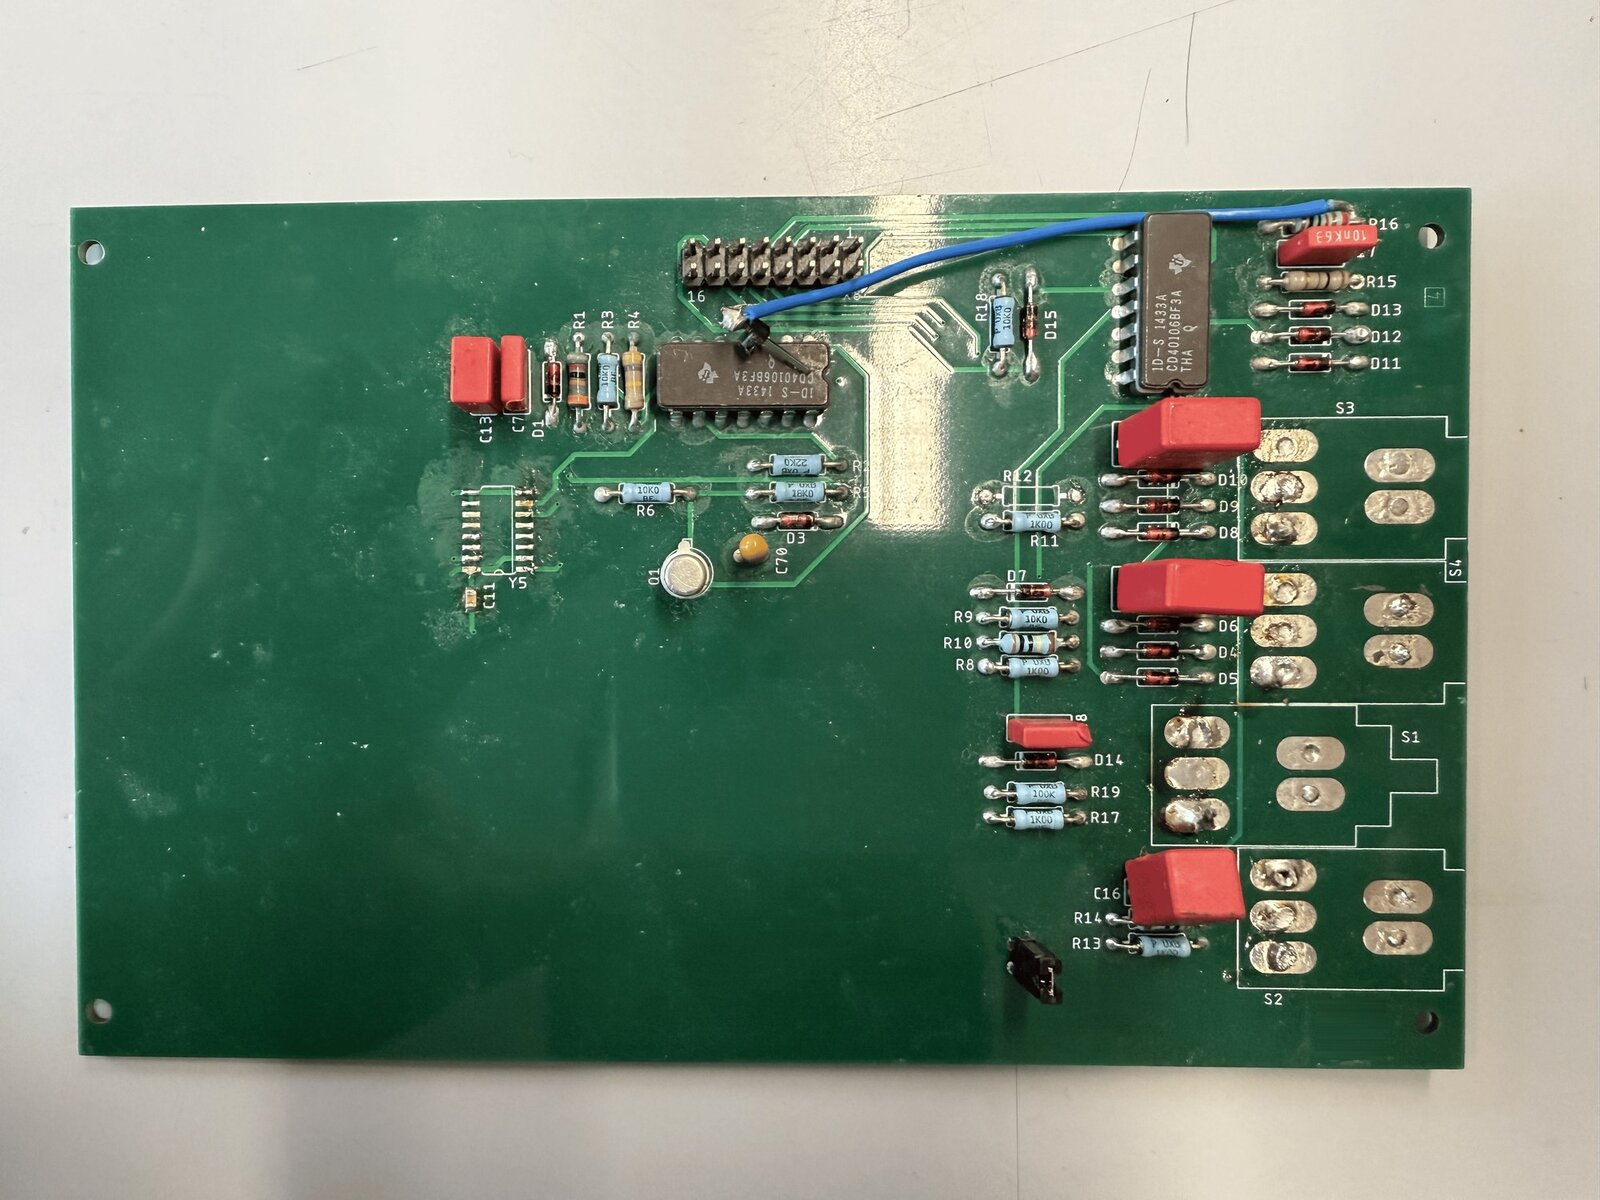
\includegraphics[width=0.75\textwidth]{photos/rev0_upper_board_top.jpg}
	\caption[Rev 0.0 Upper Board]{Inherited Rev~0.0 Upper Board, populated (top view). The blue wire was added to the prototype by hand.}
	\label{fig:rev0_upper_board}
\end{figure}

\begin{figure}[H]
	\centering
	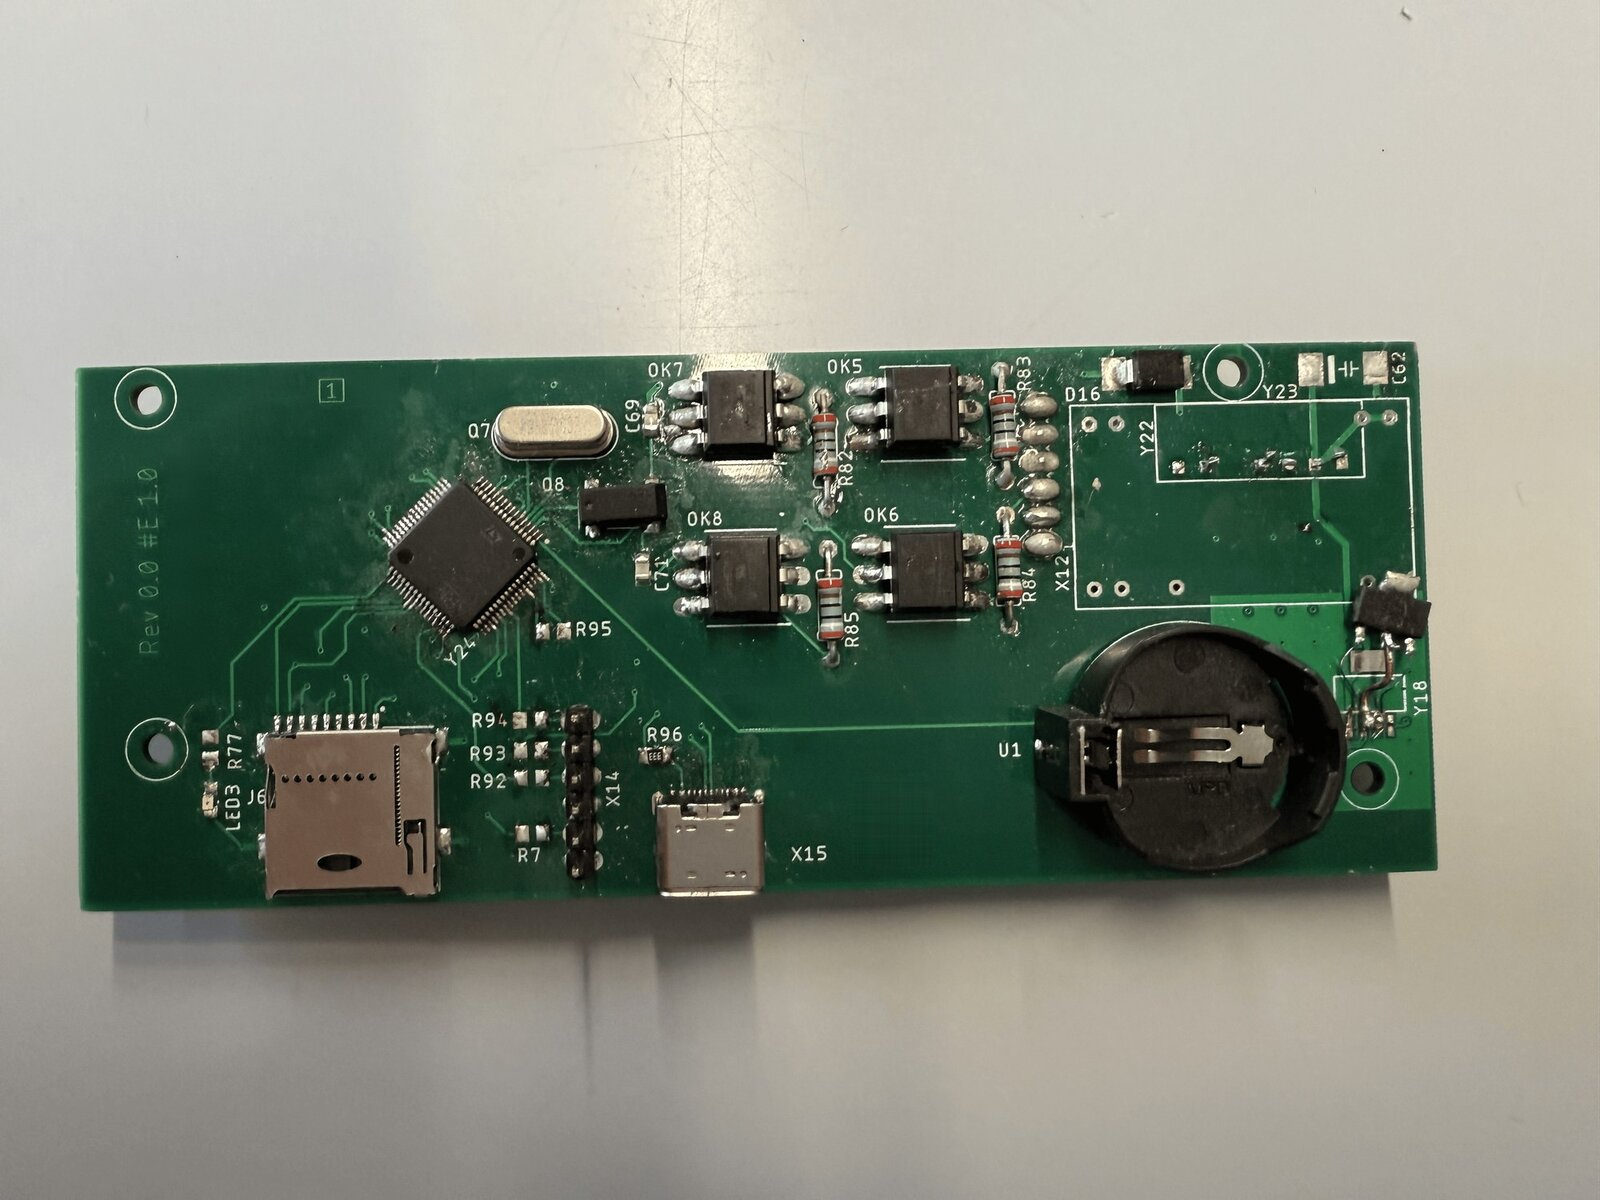
\includegraphics[width=0.75\textwidth]{photos/rev0_stm32_board_top.jpg}
	\caption[Rev 0.0 STM32 Board]{Inherited Rev~0.0 \gls{stm32} Diagnostics Board, populated (top view). Its SWD header \texttt{X14} is wired as on Rev~1.0.}
	\label{fig:rev0_stm32_board}
\end{figure}

\begin{figure}[H]
	\centering
	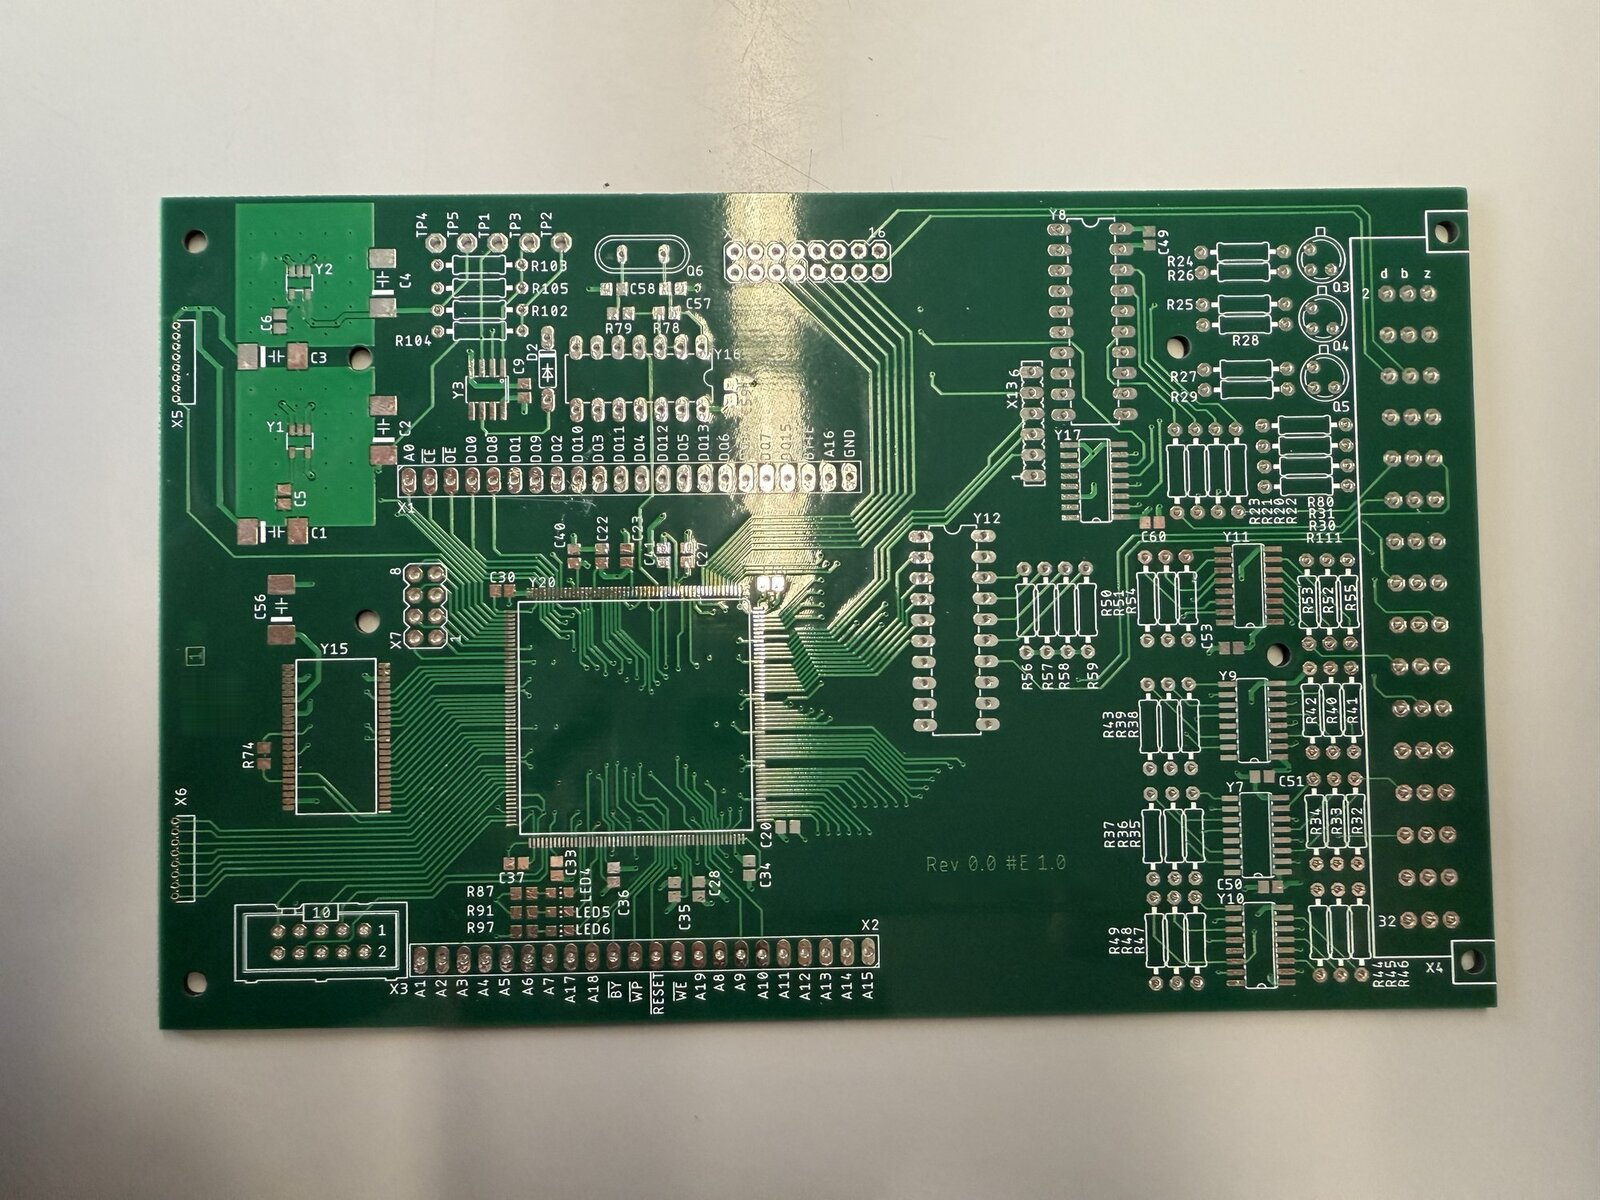
\includegraphics[width=0.75\textwidth]{photos/base_board_bare_top.jpg}
	\caption[Bare Base Board]{Base Board, unpopulated (top view). The silkscreen reads Rev~0.0: the Base Board was reused in its inherited revision (\Cref{sec:pcb_design_impl}).}
	\label{fig:bare_base_board}
\end{figure}

\begin{figure}[H]
	\centering
	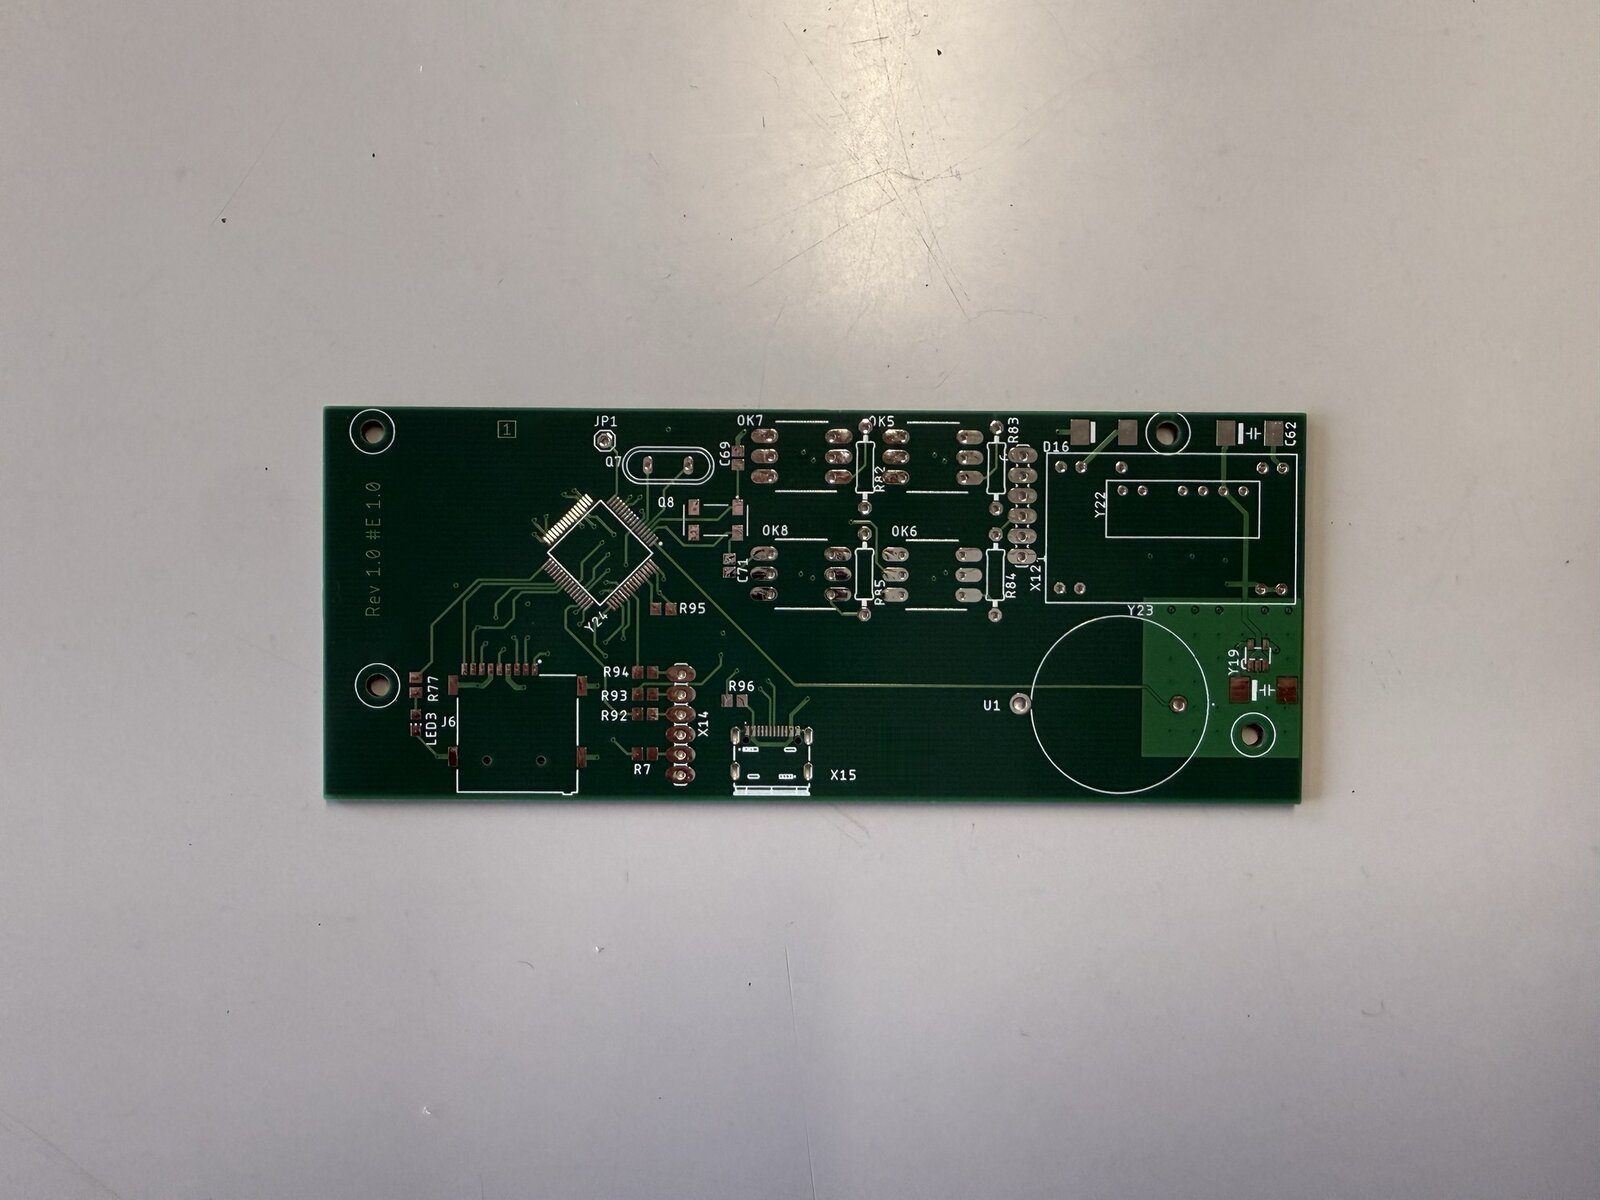
\includegraphics[width=0.75\textwidth]{photos/rev1_stm32_board_bare_top.jpg}
	\caption[Rev 1.0 Bare STM32 Board]{Corrected Rev~1.0 \gls{stm32} Diagnostics Board, unpopulated (top view), with the SWD header \texttt{X14} and its series resistors \texttt{R7} and \texttt{R92}--\texttt{R94}.}
	\label{fig:rev1_bare_stm32_board}
\end{figure}


% ------------------------------------------------------------
\section{Schematic}
\label{sec:app_schematic_sheets}

The schematic of all four boards is one Eagle project of four sheets, organised by function rather than by board. \Cref{tab:bom} lists which board carries each part.

\begin{figure}[H]
	\centering
	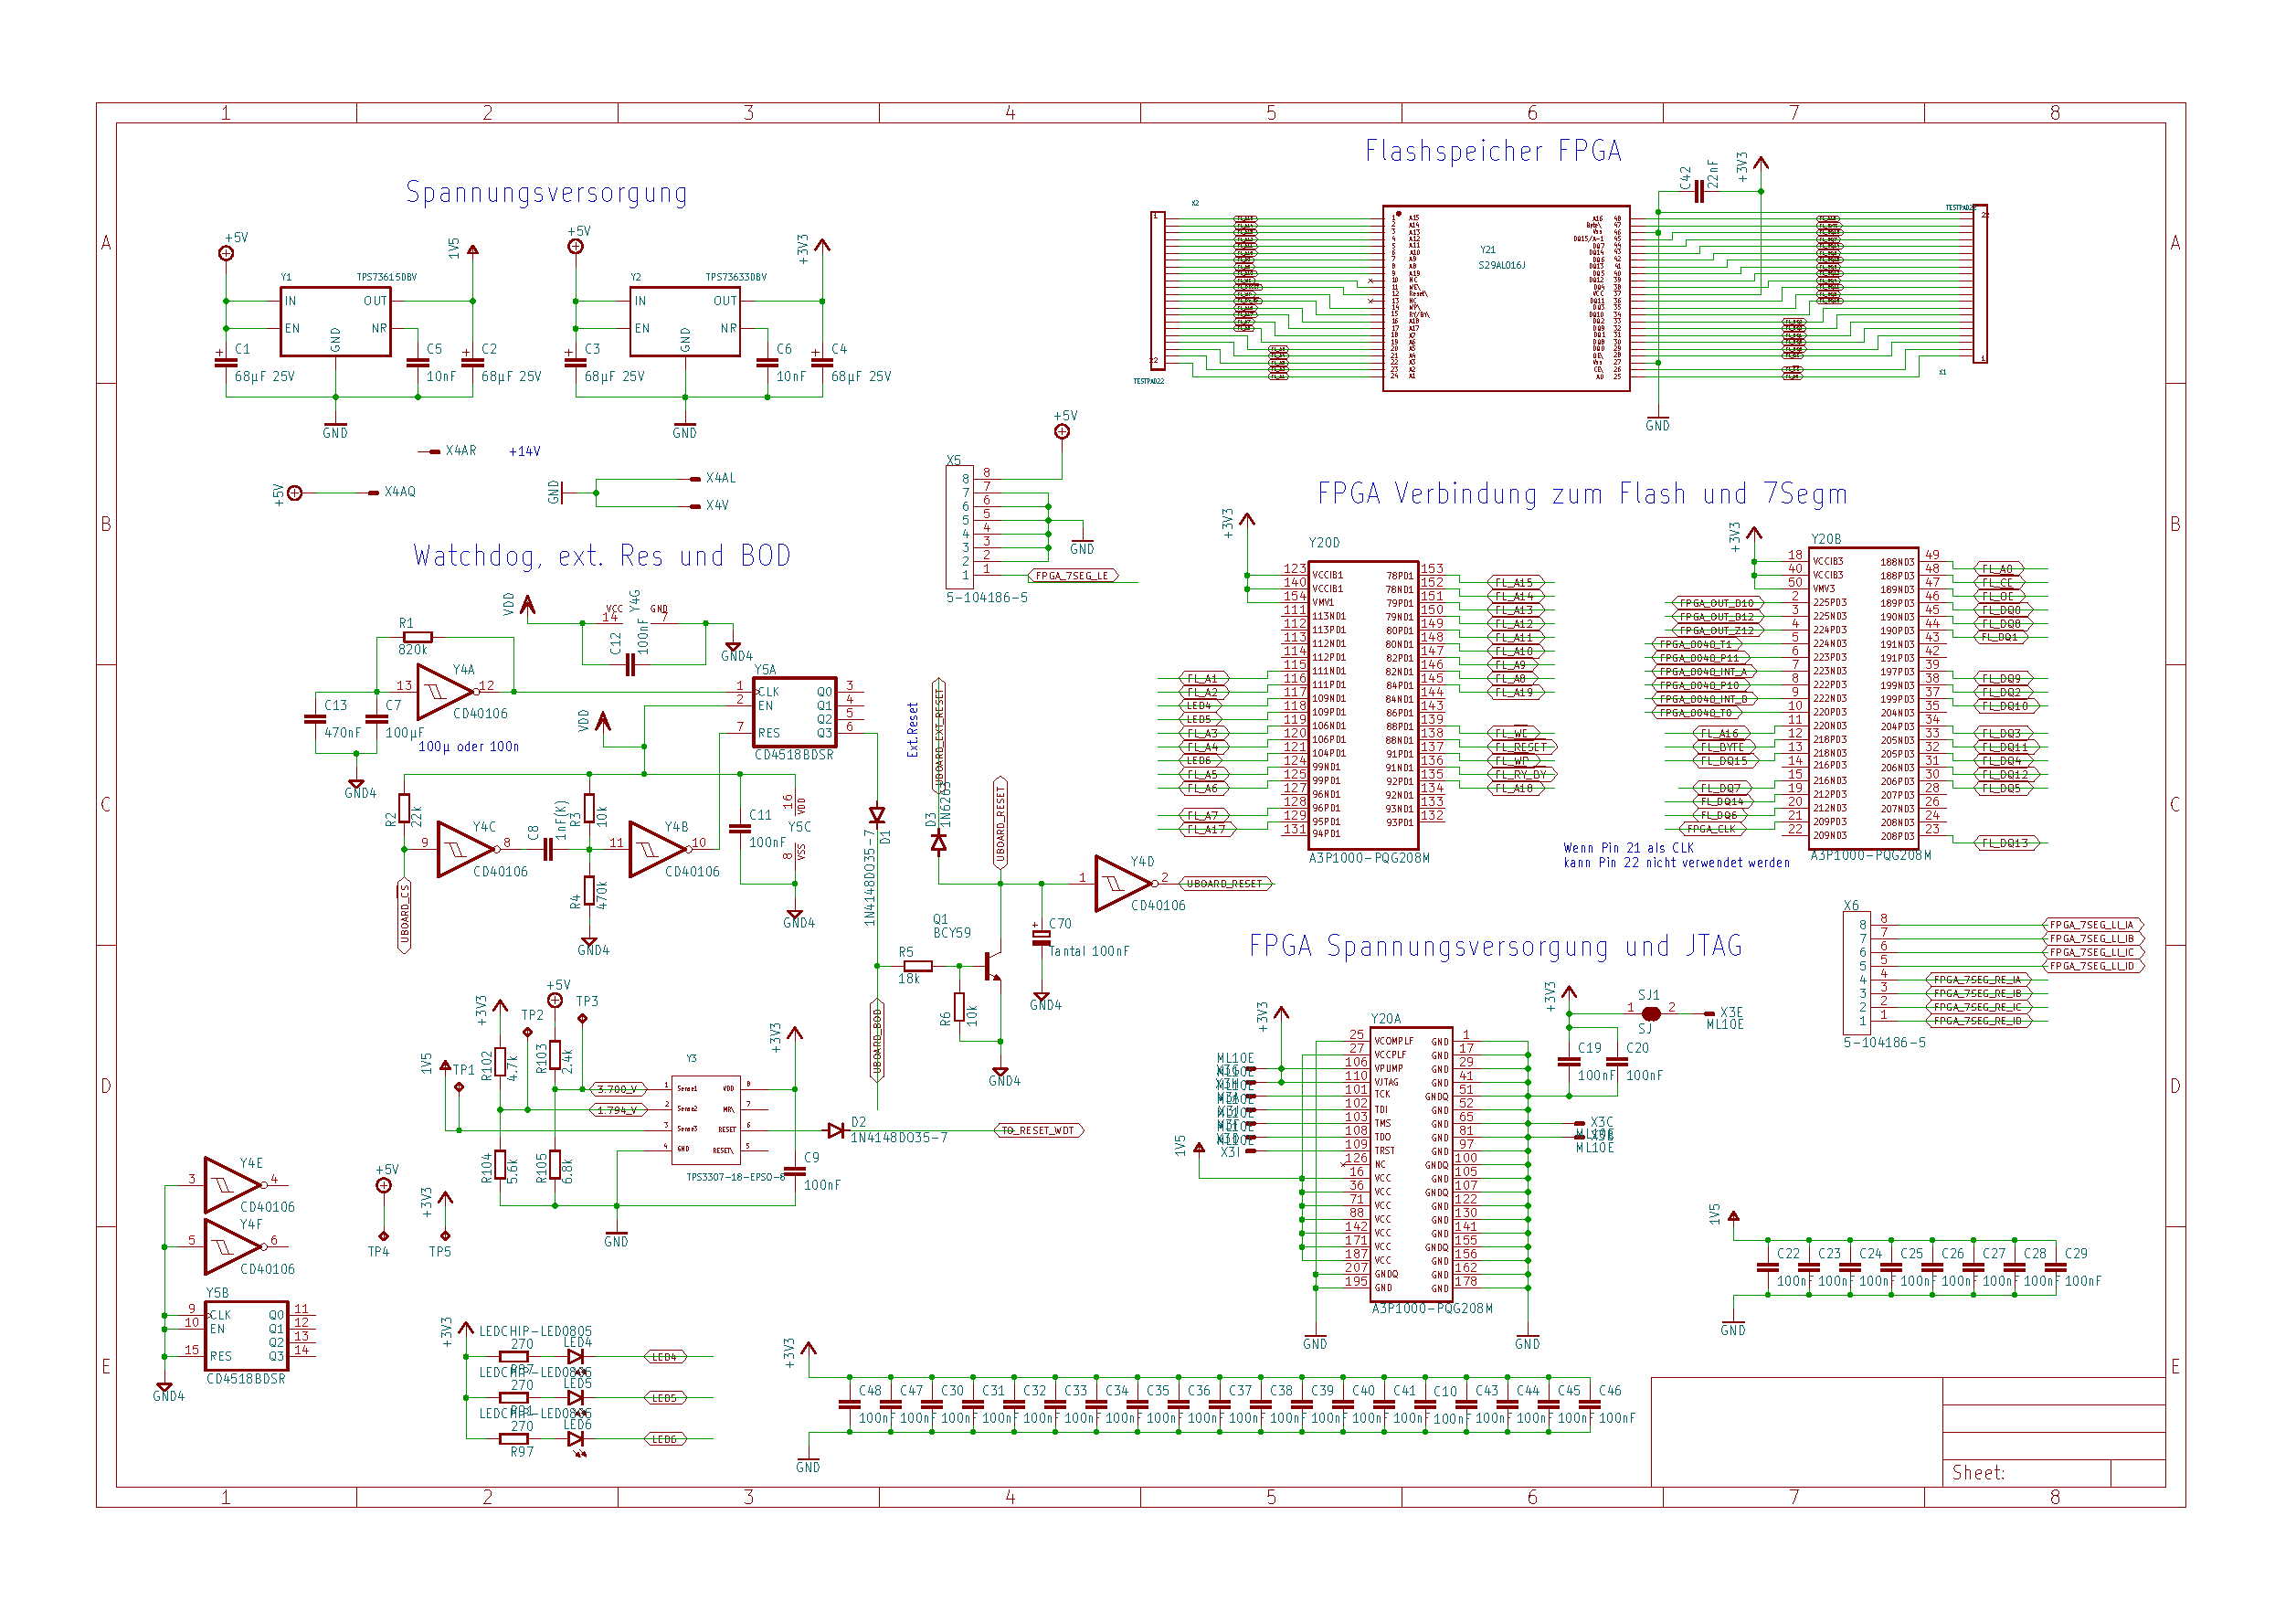
\includegraphics[trim=48 52 55 52, clip, width=0.85\textheight, angle=90]{schematic/sheet1.pdf}
	\caption[Schematic Sheet 1]{Schematic sheet~1: power supply (\texttt{Y1}, \texttt{Y2}), external watchdog with reset and brown-out detection (\texttt{Y3}--\texttt{Y5}, \texttt{Q1}), Flash~\gls{rom} (\texttt{Y21}) with its test fields \texttt{X1}/\texttt{X2}, \gls{fpga} supply and \gls{jtag} header \texttt{X3}. Rendered with KiCad from the Eagle design file of 2024. Design: Leyer~\cite{leyer2023}.}
	\label{fig:schematic_sheet1}
\end{figure}

\begin{figure}[H]
	\centering
	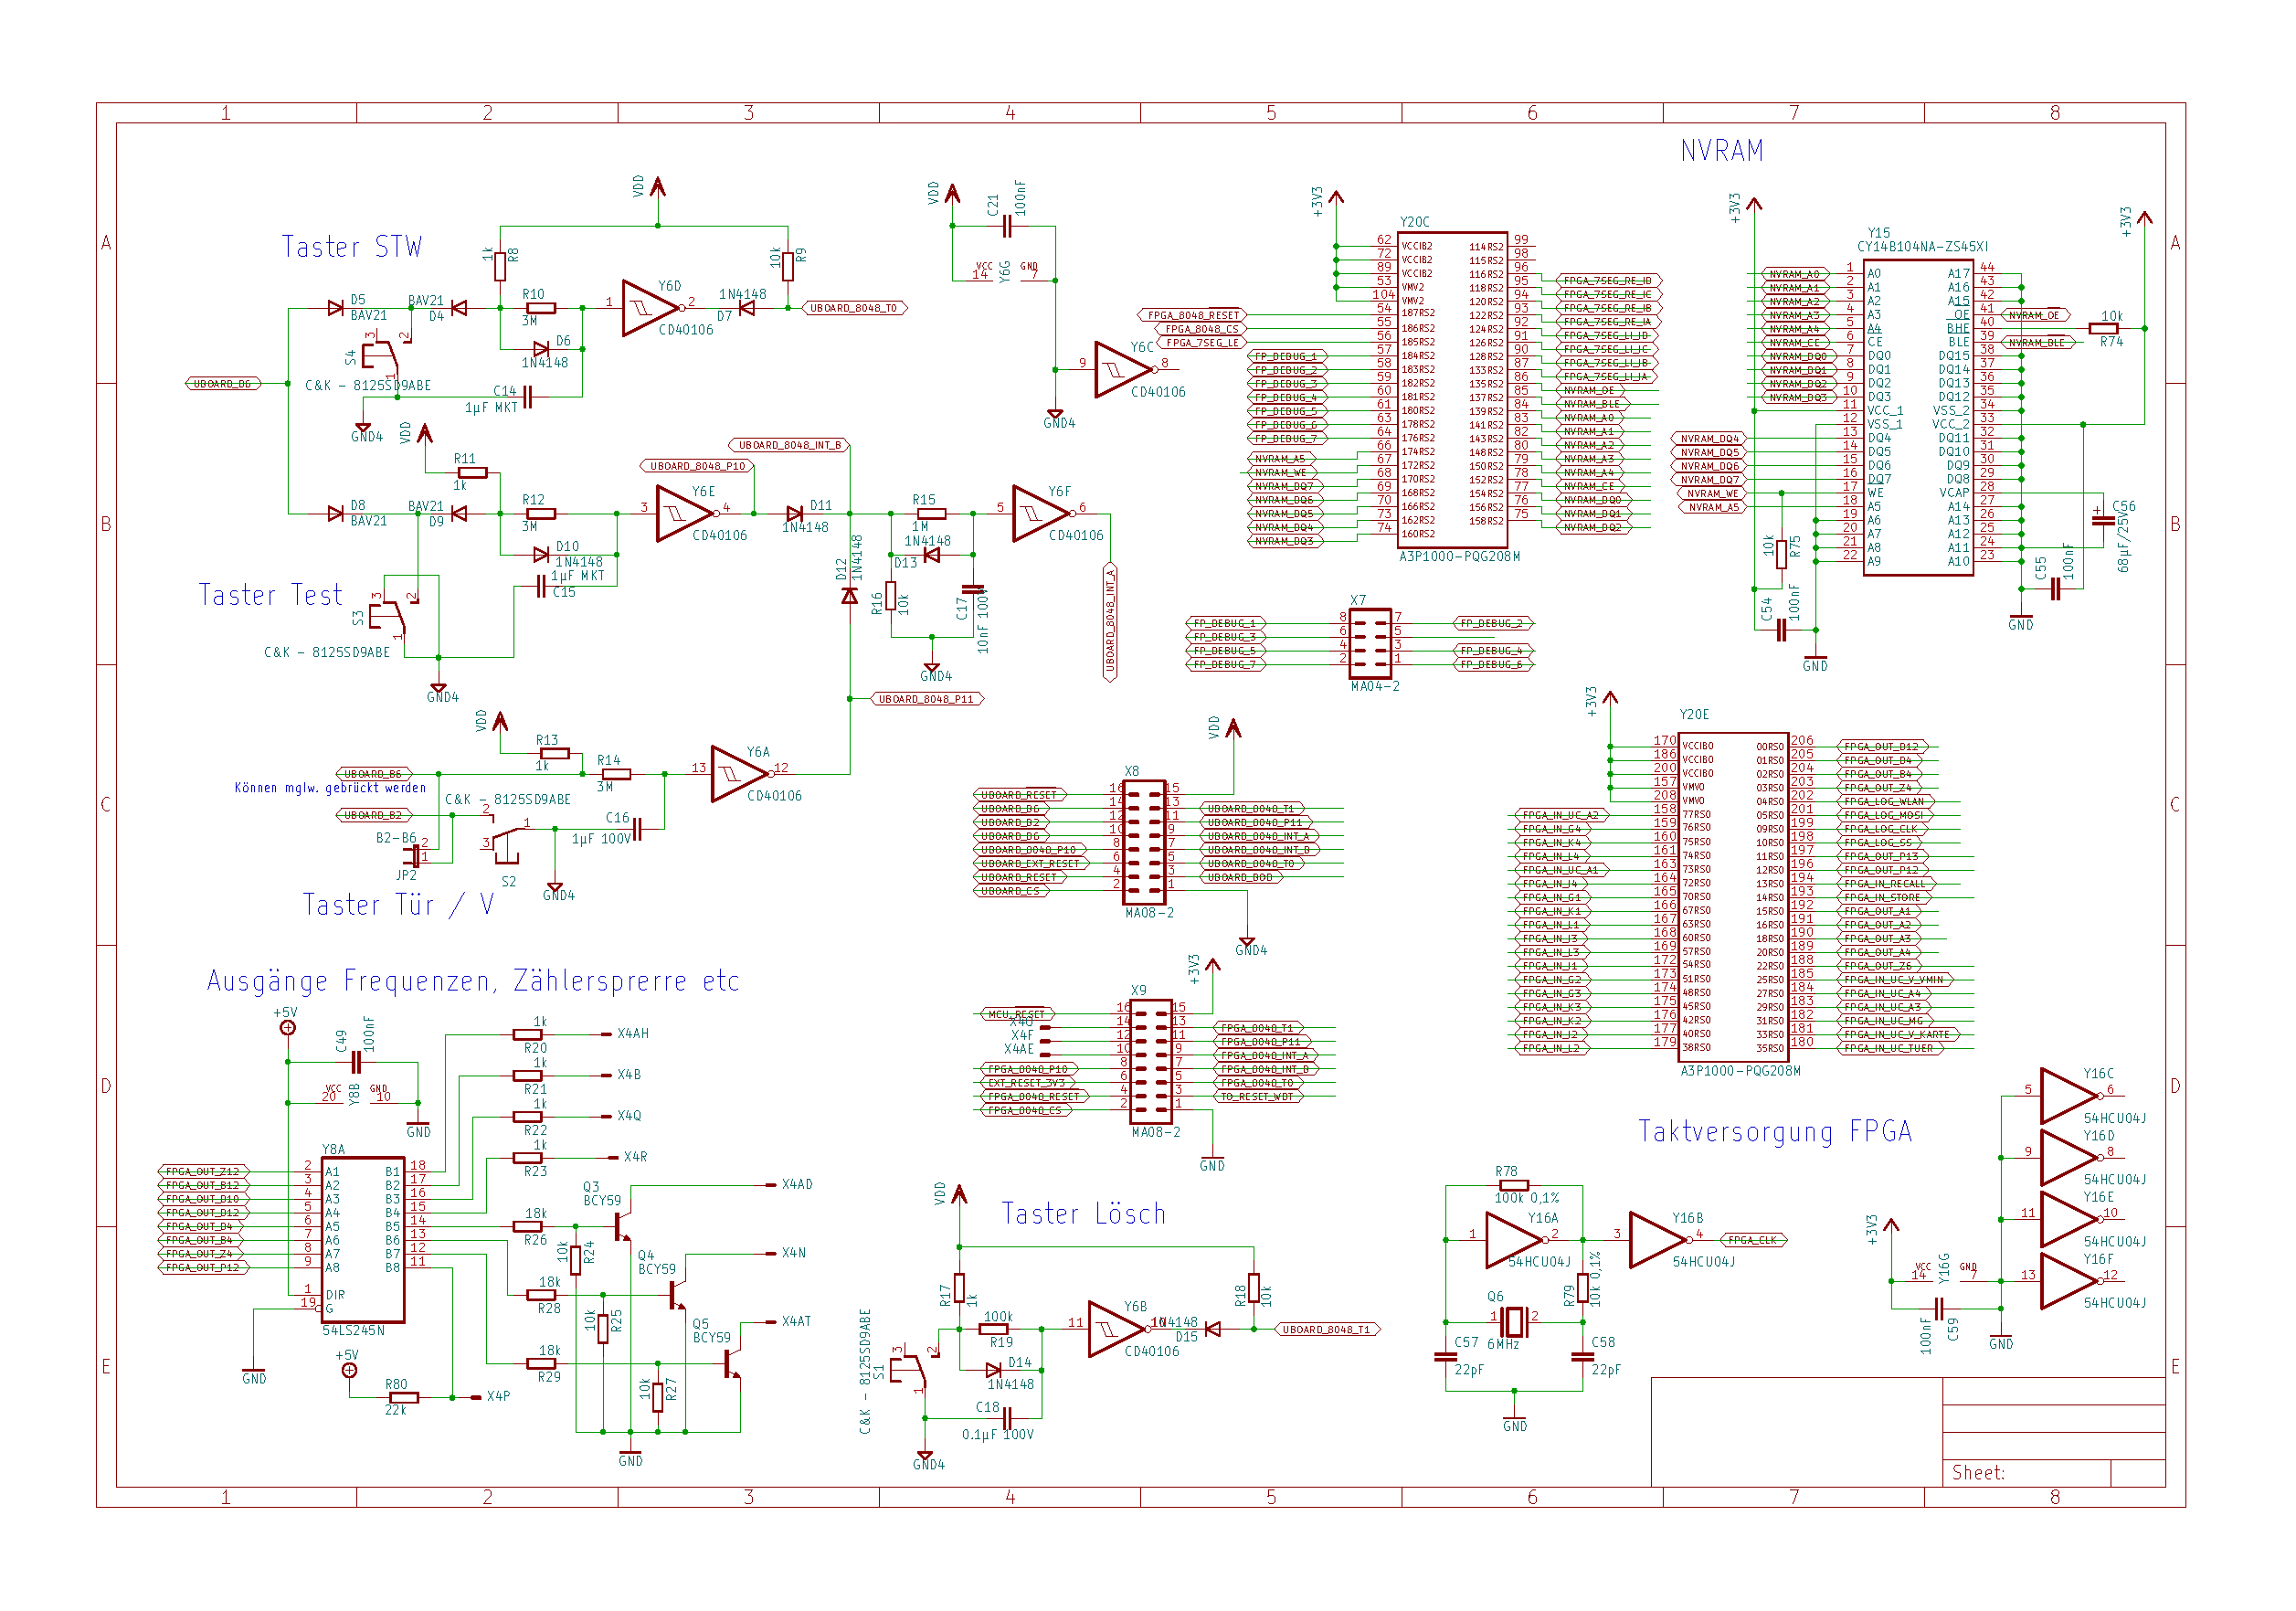
\includegraphics[trim=48 52 55 52, clip, width=0.85\textheight, angle=90]{schematic/sheet2.pdf}
	\caption[Schematic Sheet 2]{Schematic sheet~2: operator buttons with debouncing (\texttt{S1}--\texttt{S4}, \texttt{Y6}), output drivers (\texttt{Y8}, \texttt{Q3}--\texttt{Q5}), \gls{nvram} (\texttt{Y15}), \SI{6}{\mega\hertz} clock (\texttt{Y16}, \texttt{Q6}), the headers \texttt{X8} and \texttt{X9} of the ribbon cable between the Upper Board and the Base Board, and the \gls{fpga} debug header \texttt{X7}. Rendered with KiCad from the Eagle design file of 2024. Design: Leyer~\cite{leyer2023}.}
	\label{fig:schematic_sheet2}
\end{figure}

\begin{figure}[H]
	\centering
	% slightly smaller than the other sheets, so that the note on defect B6 fits below the caption
	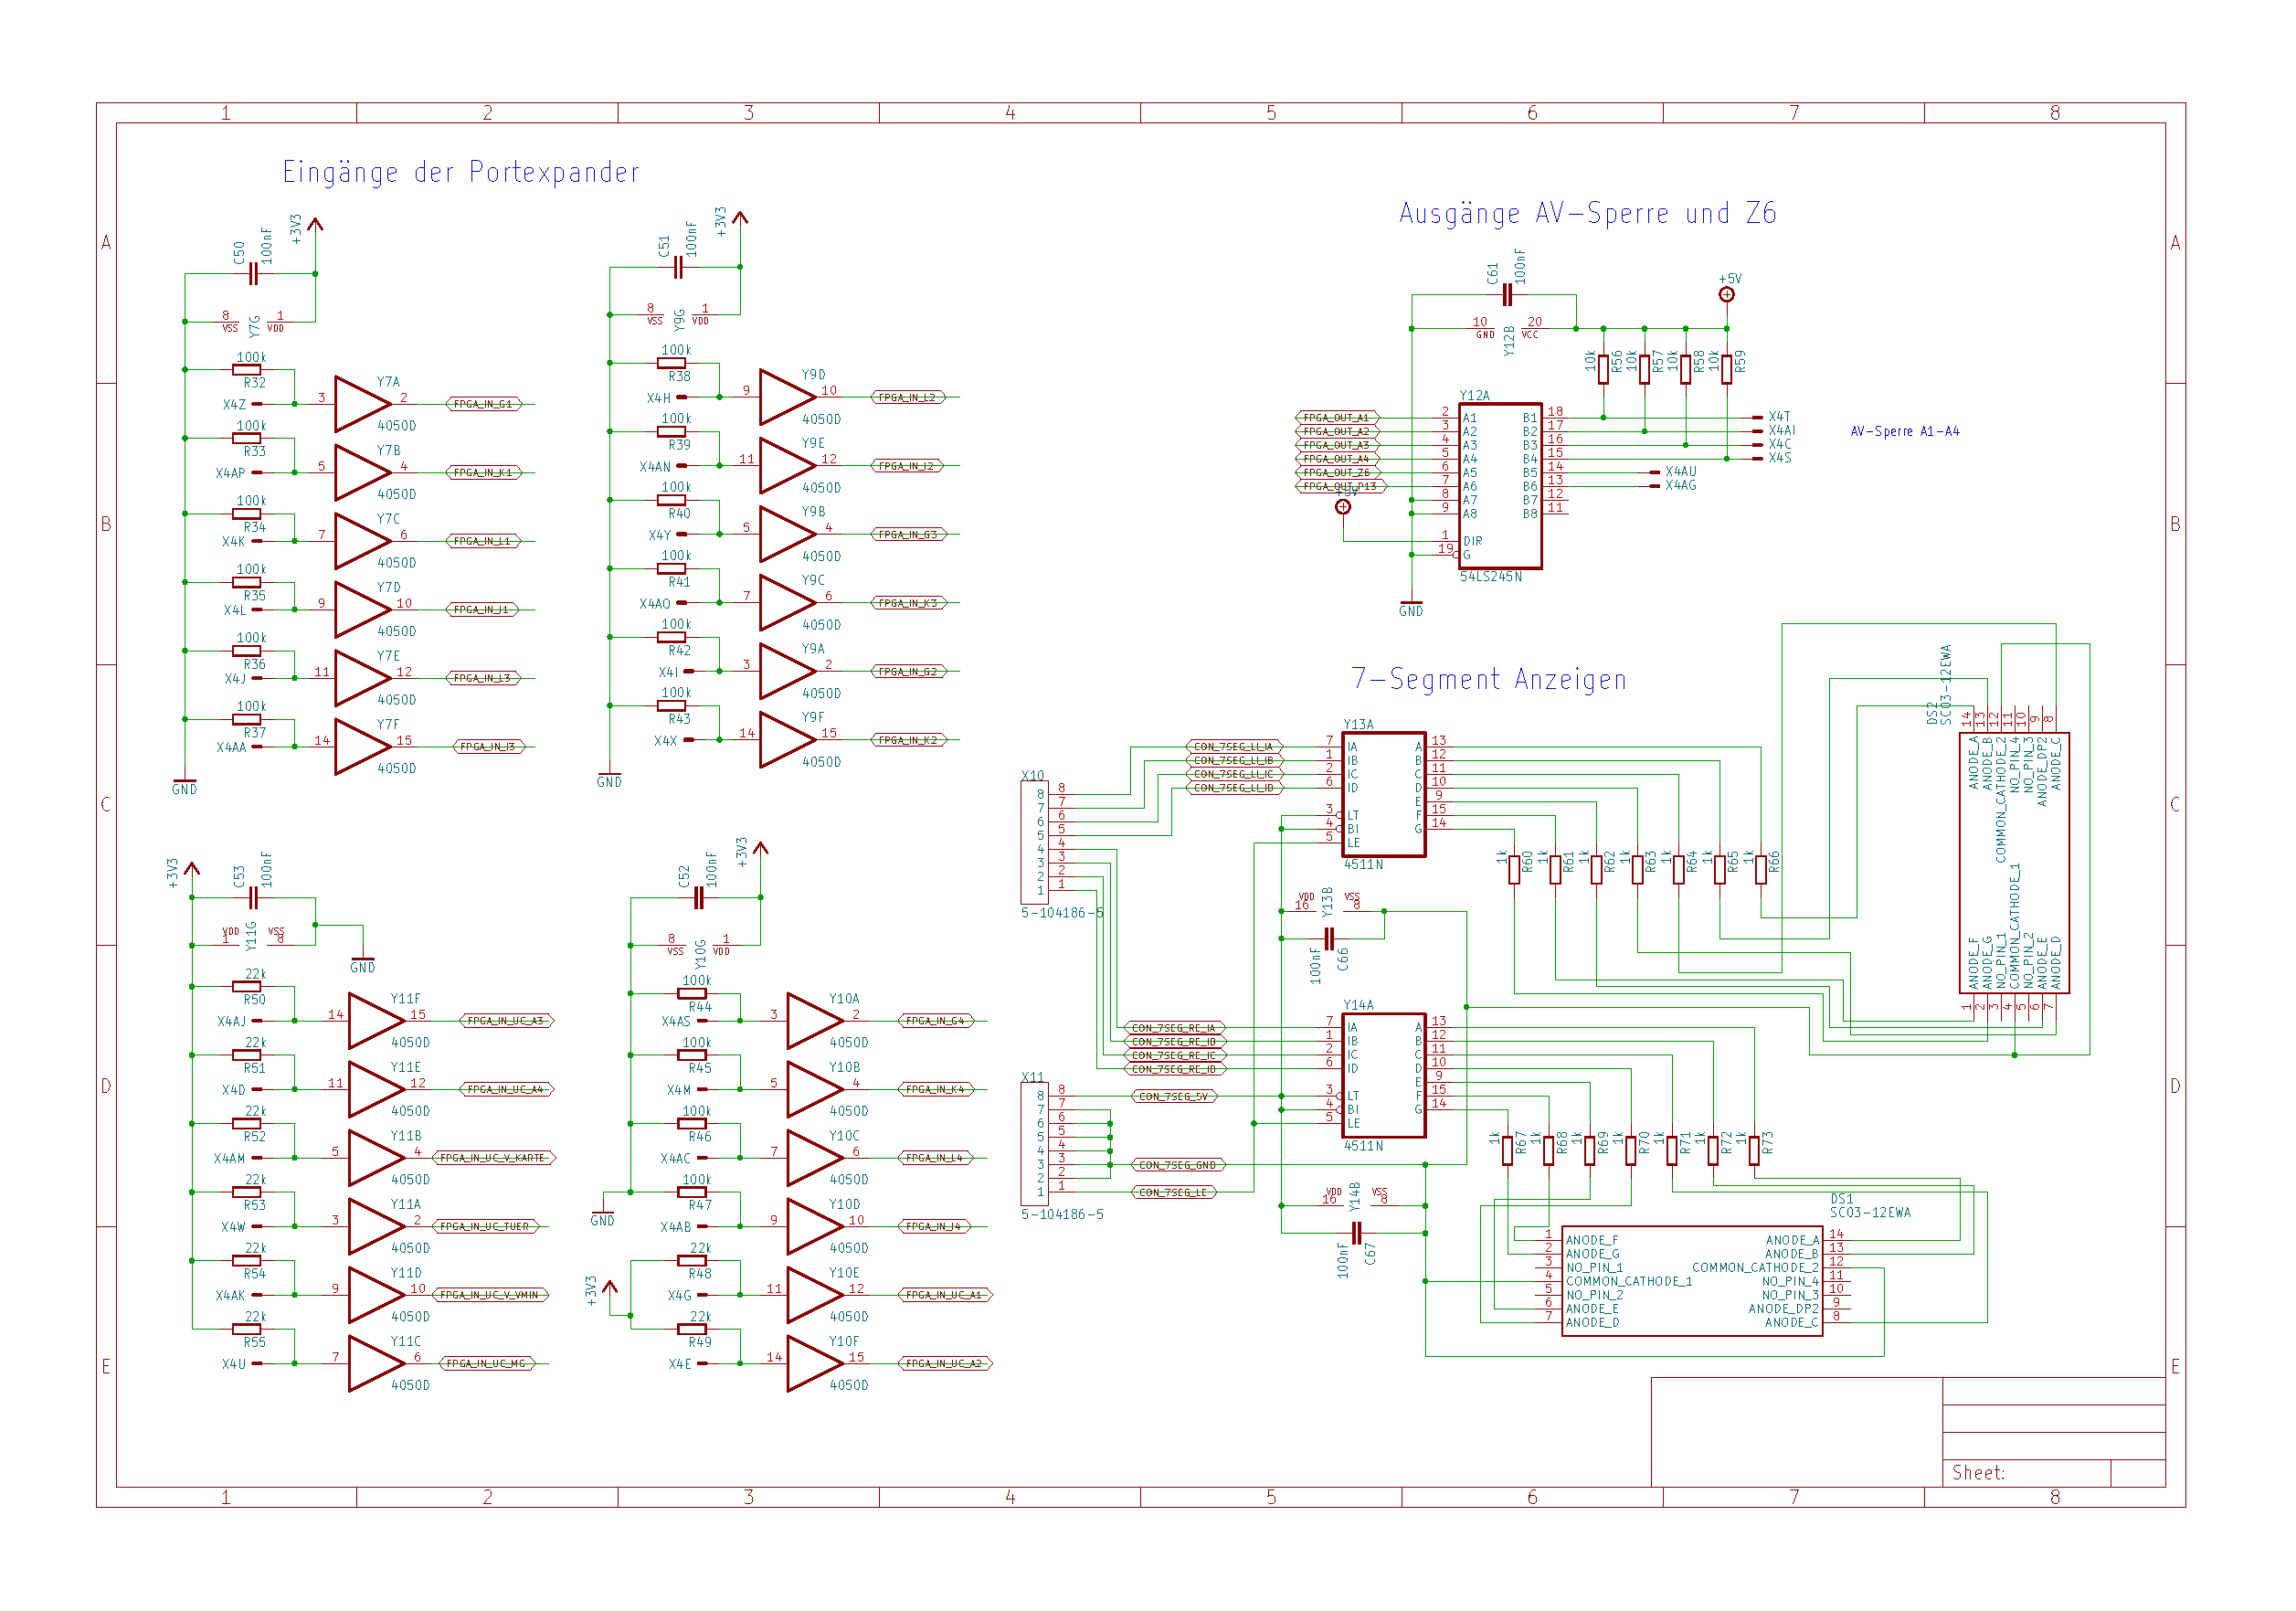
\includegraphics[trim=48 52 55 52, clip, width=0.8\textheight, angle=90]{schematic/sheet3.pdf}
	\caption[Schematic Sheet 3]{Schematic sheet~3: input level shifters for the system connector \texttt{X4} (\texttt{Y7}, \texttt{Y9}--\texttt{Y11}), output drivers (\texttt{Y12}) and the 7-segment display board with its drivers (\texttt{Y13}, \texttt{Y14}) and the \texttt{SC03-12EWA} displays \texttt{DS1} and \texttt{DS2}, with which this work replaced the end-of-life \texttt{5082-7613} displays. Rendered with KiCad from the Eagle design file of 2024. Design: Leyer~\cite{leyer2023}.}
	\label{fig:schematic_sheet3}

	\smallskip
	\begin{minipage}{\textwidth}
		\footnotesize
		Note: The driver-to-display assignment drawn on this sheet, \texttt{Y13} (left digit) to \texttt{DS2} and \texttt{Y14} (right digit) to \texttt{DS1}, is reversed against the design files of 2023, in which \texttt{Y13} drives the display at the position of \texttt{DS1}; it produced defect B6 (\Cref{tab:bug_taxonomy}), which the follow-on team worked around in \texttt{atop.vhd}~\cite[p.~13]{savchuk2025}. The corrected \texttt{atop.vhd} is not archived.
	\end{minipage}
\end{figure}

\begin{figure}[H]
	\centering
	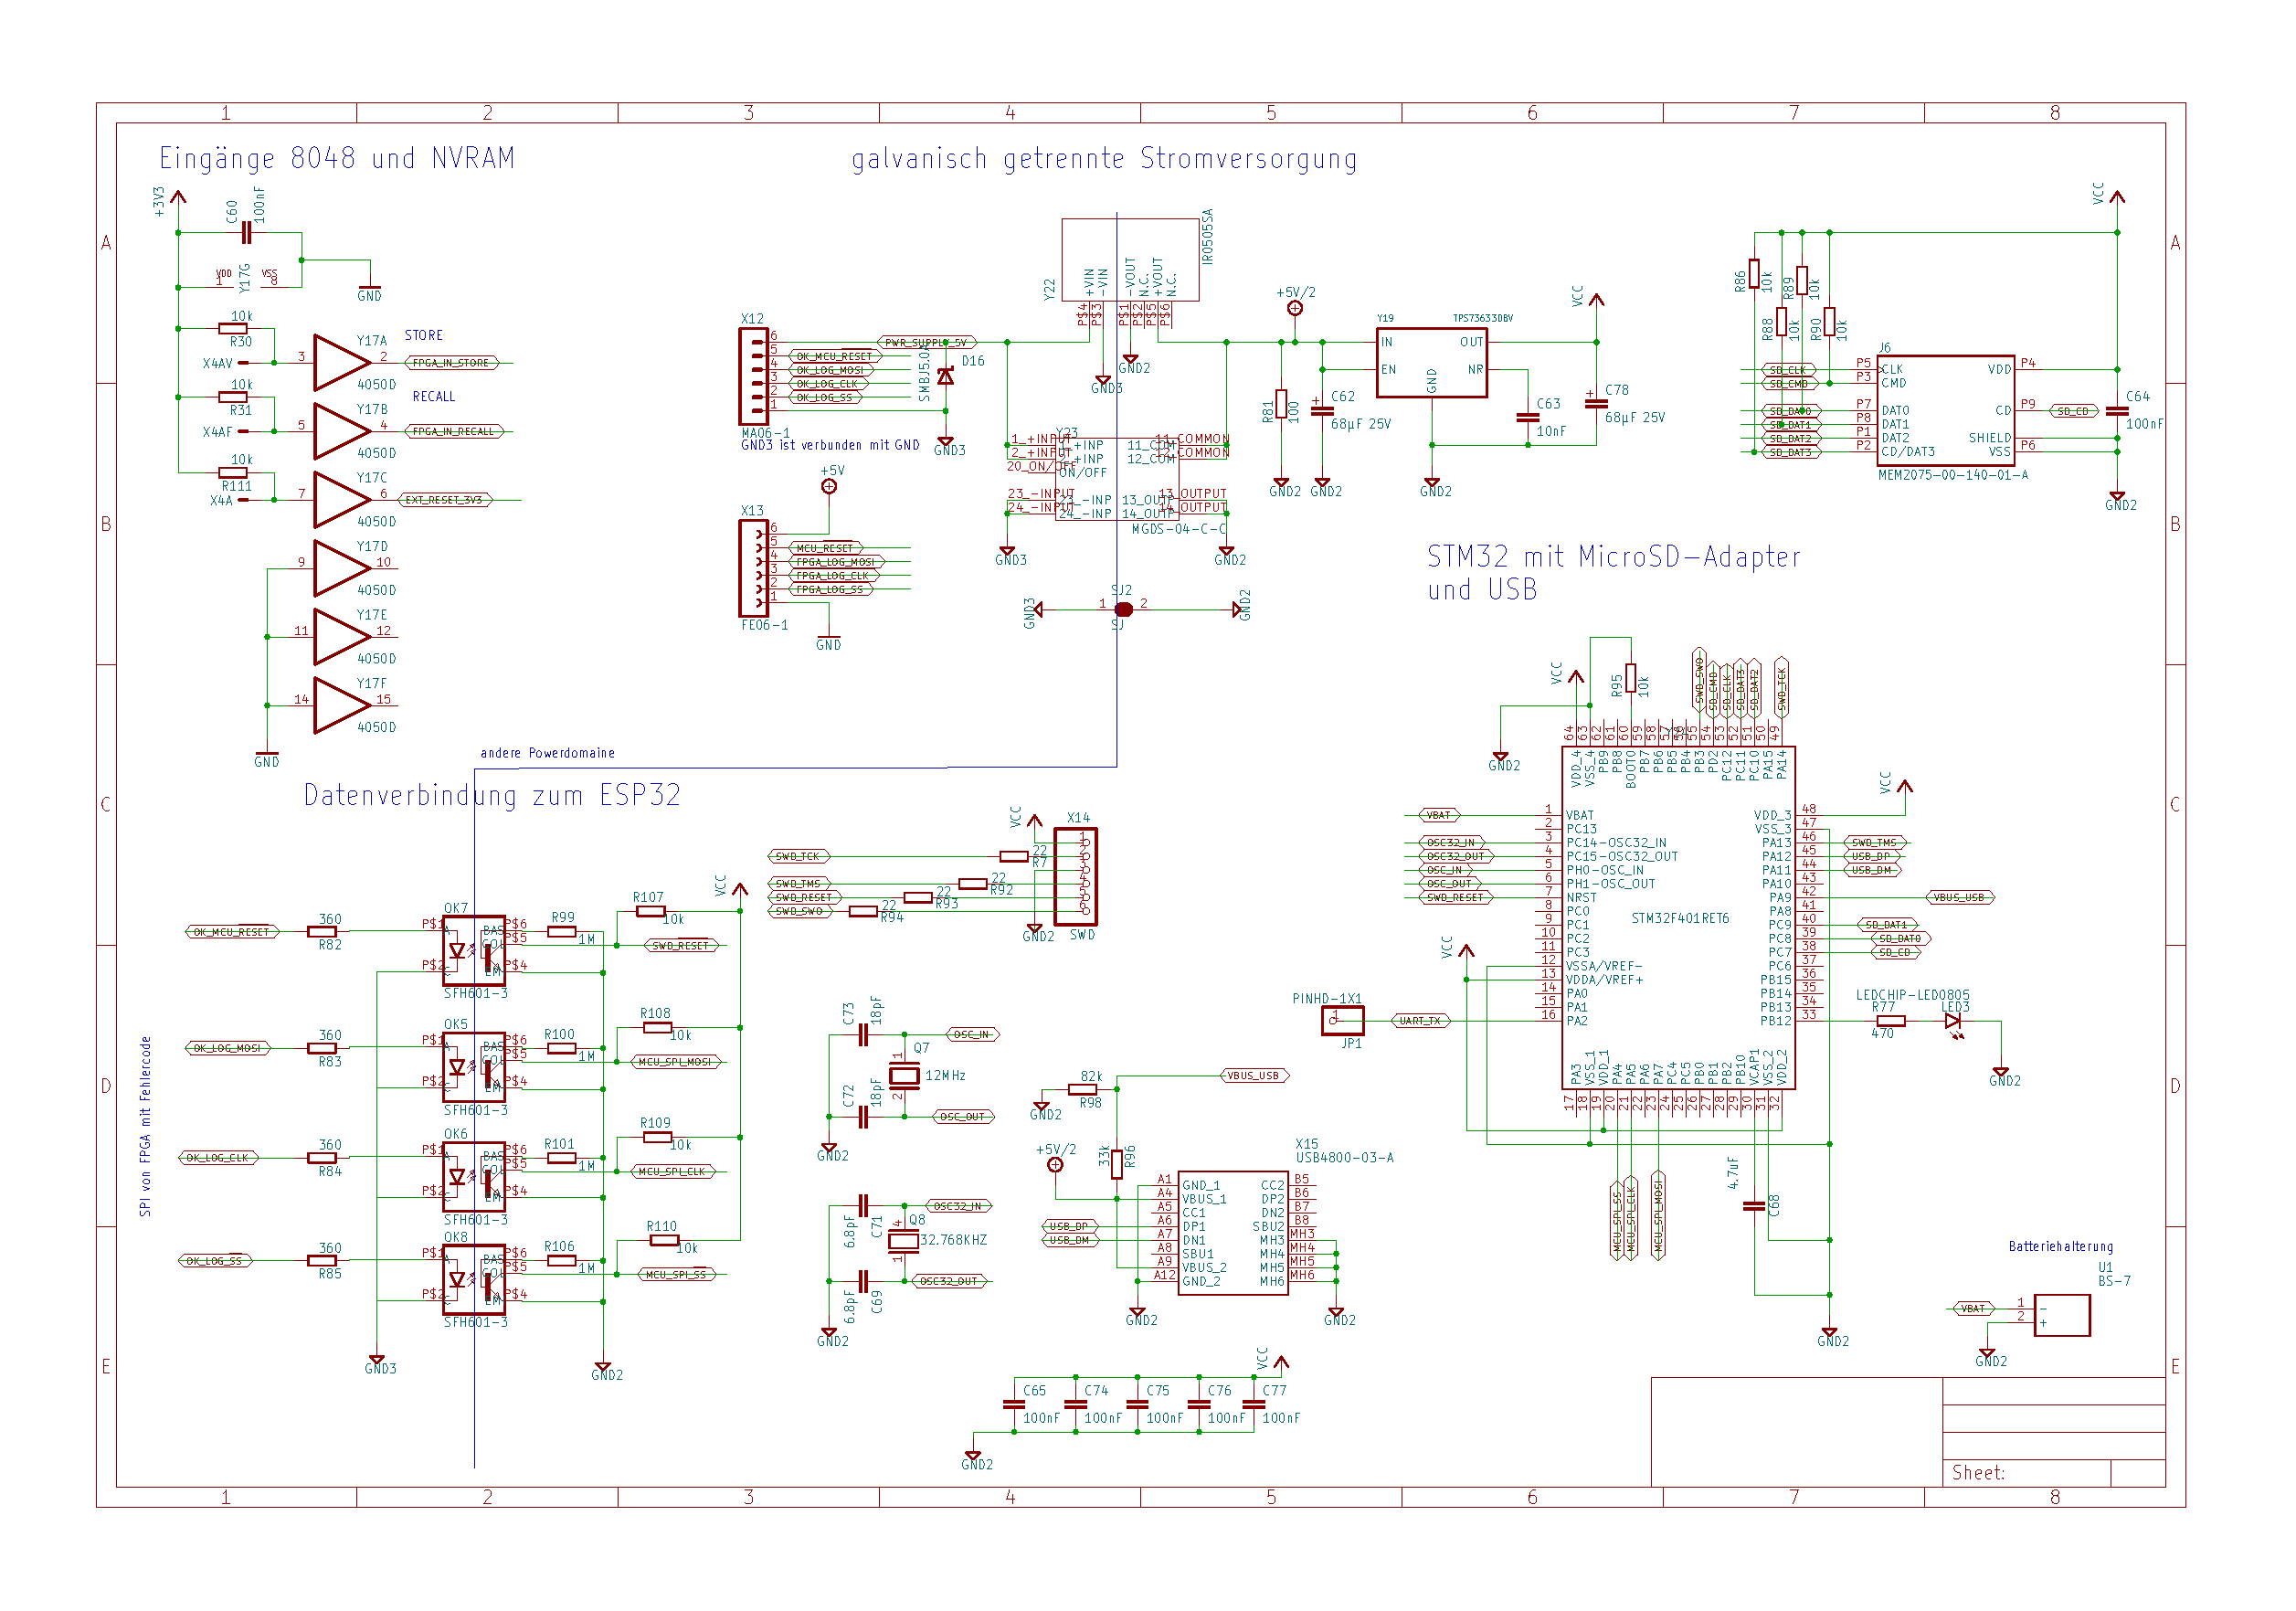
\includegraphics[trim=48 52 55 52, clip, width=0.85\textheight, angle=90]{schematic/sheet4.pdf}
	\caption[Schematic Sheet 4]{Schematic sheet~4: \gls{stm32} Diagnostics Board with isolated supply (\texttt{Y19}, \texttt{Y22}, \texttt{Y23}), optocoupled link (\texttt{OK5}--\texttt{OK8}), MicroSD socket (\texttt{J6}), \gls{usb} Type-C connector (\texttt{X15}), SWD header (\texttt{X14}) and \gls{rtc} crystal (\texttt{Q8}); the block \enquote{Eingänge 8048 und NVRAM} (inputs of the 8048 and the~\gls{nvram}) holds the Base Board input buffer \texttt{Y17}. The label \enquote{Datenverbindung zum ESP32} is left over from an earlier variant based on an ESP32 module. Rendered with KiCad from the Eagle design file of 2024. Design: Leyer~\cite{leyer2023}.}
	\label{fig:schematic_sheet4}
\end{figure}

\clearpage

% ------------------------------------------------------------
\section{Base Board (Unterplatine) Layout}
\label{sec:app_base_board_schematics}

\begin{figure}[H]
	\centering
	\includegraphicsowngroup[width=0.9\textwidth]{layout/top/unterplatine.pdf}
	\caption[Base Board Layout (Top)]{Base Board (Rev~0.0) PCB layout, top view, showing the component placement. Rendered with KiCad from the Eagle design file of 2024, without the third-party logo and board designation. Design: Leyer~\cite{leyer2023}.}
	\label{fig:base_layout_top}
\end{figure}

\begin{figure}[H]
	\centering
	\includegraphicsowngroup[width=0.9\textwidth]{layout/bottom/unterplatine.pdf}
	\caption[Base Board Layout (Bottom)]{Base Board (Rev~0.0) PCB layout, bottom view (mirrored). Rendered with KiCad from the Eagle design file of 2024, without the third-party logo. Design: Leyer~\cite{leyer2023}.}
	\label{fig:base_layout_bottom}
\end{figure}

\clearpage

% ------------------------------------------------------------
\section[Upper Board (Oberplatine) and LED Board Layouts]{Upper Board (Oberplatine) and LED Board\\Layouts}
\label{sec:app_upper_board_schematics}

\begin{figure}[H]
	\centering
	\includegraphicsowngroup[width=0.9\textwidth]{layout/top/oberplatine.pdf}
	\caption[Upper Board Layout (Top)]{Upper Board (Rev~1.0) PCB layout, top view. Rendered with KiCad from the Eagle design file of 2024, without the third-party logo and board designation. Design: Leyer~\cite{leyer2023}.}
	\label{fig:upper_layout_top}
\end{figure}

\begin{figure}[H]
	\centering
	\includegraphicsowngroup[width=0.9\textwidth]{layout/bottom/oberplatine.pdf}
	\caption[Upper Board Layout (Bottom)]{Upper Board (Rev~1.0) PCB layout, bottom view (mirrored). Rendered with KiCad from the Eagle design file of 2024, without the third-party logo. Design: Leyer~\cite{leyer2023}.}
	\label{fig:upper_layout_bottom}
\end{figure}

\phantomsection
\label{sec:app_led_board_schematics}
\begin{figure}[H]
	\centering
	\includegraphicsowngroup[width=0.9\textwidth]{layout/top/led.pdf}
	\caption[LED Board Layout (Top)]{LED Board (Rev~1.0) PCB layout, top view. Rendered with KiCad from the Eagle design file of 2024, without the third-party logo and board designation. Design: Leyer~\cite{leyer2023}.}
	\label{fig:led_layout_top}
\end{figure}

\begin{figure}[H]
	\centering
	\includegraphicsowngroup[width=0.9\textwidth]{layout/bottom/led.pdf}
	\caption[LED Board Layout (Bottom)]{LED Board (Rev~1.0) PCB layout, bottom view (mirrored), with the \texttt{SC03-12EWA} displays \texttt{DS1} and \texttt{DS2}. Rendered with KiCad from the Eagle design file of 2024. Design: Leyer~\cite{leyer2023}.}
	\label{fig:led_layout_bottom}
\end{figure}


% ------------------------------------------------------------
\section{STM32 Diagnostics Board Layout}
\label{sec:app_stm32_board_schematics}

\begin{figure}[H]
	\centering
	\includegraphicsowngroup[width=0.9\textwidth]{layout/top/stm32.pdf}
	\caption[STM32 Board Layout (Top)]{\gls{stm32} Diagnostics Board (Rev~1.0) PCB layout, top view. Rendered with KiCad from the Eagle design file of 2024, without the third-party logo and board designation. Design: Leyer~\cite{leyer2023}.}
	\label{fig:stm32_layout_top}
\end{figure}

\begin{figure}[H]
	\centering
	\includegraphicsowngroup[width=0.9\textwidth]{layout/bottom/stm32.pdf}
	\caption[STM32 Board Layout (Bottom)]{\gls{stm32} Diagnostics Board (Rev~1.0) PCB layout, bottom view (mirrored). Rendered with KiCad from the Eagle design file of 2024, without the third-party logo. Design: Leyer~\cite{leyer2023}.}
	\label{fig:stm32_layout_bottom}
\end{figure}


% ------------------------------------------------------------
\section{Connectors}
\label{sec:app_connectors}
The boards are connected by standard pin headers and sockets. The Base Board carries the LED Board on two TE AMPMODU System~50 headers (\texttt{X5}/\texttt{X6} mating with \texttt{X10}/\texttt{X11})~\cite{te_ampmodu_sys50} and the \gls{stm32} Diagnostics Board on a six-pin header pair (\texttt{X13}/\texttt{X12}); the Upper Board is connected by a ribbon cable between the 2$\times$8 headers \texttt{X9} and \texttt{X8}. The vehicle side is reached through the 48-pin DIN~41612 type~F system connector \texttt{X4}.

% back to the page layout of the other chapters
\flushbottom

% ============================================================
% Appendix B: Bill of Materials (BOM) and Design Rules
% ============================================================
\chapter{Bill of Materials (BOM) and Design Rules}
\label{app:bom_drc}

This appendix lists the parts of the retrofitted hardware modules and gives the design rules of their layouts.

% ------------------------------------------------------------
\section{Bill of Materials (BOM)}
\label{sec:app_bom}

\Cref{tab:bom} lists the parts of the Rev~1.0 design board by board; the fitted Base Board is the inherited Rev~0.0 board. The table continues Leyer's bill of materials for Rev~1.0~\cite{leyer2023} and was compiled from the inspection of the populated boards and from the project's sourcing files and datasheets, and checked against the Rev~1.0 schematic and layout files. The group headings give the board that carries a part, which may differ from the schematic sheet that shows it (\Cref{sec:app_schematic_sheets}). Parts of one board share a row only where the Rev~1.0 layout gives them the same value and package and the Rev~1.0 bill of materials the same part number; \enquote{unknown} marks a manufacturer or part number that the sources do not give. Where the sources disagree, or the Rev~1.0 bill of materials does not list a part, the description or a note says so.

\begingroup
\small
\setlength{\tabcolsep}{4pt}
\setlength{\LTpost}{0.5\baselineskip}
% Ragged-right columns; a designator range is kept on one line (\mbox); the group
% headings give the board, so the table needs no column for it; space, not a rule,
% separates the groups, so a page break between them does not double the rule of the foot
\begin{longtable}{@{} >{\raggedright\arraybackslash}p{0.16\linewidth} >{\centering\arraybackslash}p{0.045\linewidth} >{\raggedright\arraybackslash}p{0.148\linewidth} >{\raggedright\arraybackslash}p{0.205\linewidth} >{\raggedright\arraybackslash}p{0.371\linewidth} @{}}
	\caption{Bill of Materials (Rev~1.0 design; the fitted Base Board is Rev~0.0)} \label{tab:bom} \\
	\toprule
	Designator(s) & Qty & Manufacturer & Part Number & Description \\
	\midrule
	\endfirsthead
	\caption[]{Bill of Materials (Rev~1.0 design; the fitted Base Board is Rev~0.0) (Continued)} \\
	\toprule
	Designator(s) & Qty & Manufacturer & Part Number & Description \\
	\midrule
	\endhead
	\midrule
	\multicolumn{5}{r@{}}{\textit{Continued on next page}} \\
	\endfoot
	\bottomrule
	\endlastfoot

	\multicolumn{5}{@{}l}{\textit{LED Display Board}} \\*
	DS1, DS2$^{a}$ & 2 & Kingbright & \texttt{SC03-12EWA} & 7-Segment Display Red 0.3" Common Cathode \\
	Y13, Y14 & 2 & TI & \texttt{CD4511BE} & BCD-to-7-Segment Latch/Decoder/Driver (DIL16) \\
	\mbox{R60--R73} & 14 & Yageo & \texttt{MF0207FTE52-1K} & Resistor \SI{1}{\kilo\ohm} \SI{0.6}{\watt} (Segment Limit) \\
	C66, C67 & 2 & Kyocera AVX & \texttt{08055C104K4T2A} & Capacitor Ceramic \SI{100}{\nano\farad} 0805 \\
	X10, X11 & 2 & TE & \texttt{5-104186-5} & Header, 8 Positions, \SI{1.27}{\milli\metre} (AMPMODU System 50), to Base Board \\
	\addlinespace[0.8em]
	\multicolumn{5}{@{}l}{\textit{STM32 Diagnostics Board}} \\*
	Y24 & 1 & STMicro & \texttt{STM32F401RET6} & Microcontroller Arm\textsuperscript{\textregistered}~Cortex\textsuperscript{\textregistered}-M4 (LQFP64) \\
	Y19$^{b}$ & 1 & TI & \texttt{TPS73633DBVT} & \SI{3.3}{\volt} Low-Dropout (\acrshort{ldo}) Regulator (Isolated Domain) \\
	\mbox{OK5--OK8}$^{c}$ & 4 & Vishay & \texttt{SFH601-3} & Optocoupler (SPI and NRST Isolation) \\
	Y22 & 0 & XP Power & \texttt{IR0505SA} & Isolated DC/DC Converter \SI{5}{\volt} to \SI{5}{\volt} (Alternative to Y23, Not Fitted) \\
	Y23 & 1 & Gaia & \texttt{MGDS04-C-C} & Isolated DC/DC Converter \SI{5}{\volt} to \SI{5}{\volt} \\
	J6 & 1 & GCT & \texttt{MEM2075-\allowbreak{}00-\allowbreak{}140-\allowbreak{}01-\allowbreak{}A} & MicroSD Card Socket (Push-Push) \\
	X15 & 1 & GCT & \texttt{USB4800-03-A} & USB Type-C Connector \\
	U1 & 1 & MPD & \texttt{BS-7} & RTC Battery Holder (CR2032) \\
	Q7 & 1 & ECS & \texttt{ECS-120-20-4X-EM} & Crystal \SI{12}{\mega\hertz} \\
	Q8 & 1 & Abracon & \texttt{ABS25-\allowbreak{}32.768KHZ-\allowbreak{}6-\allowbreak{}T} & Crystal \SI{32.768}{\kilo\hertz} \\
	X12 & 1 & unknown & unknown & Connector to Base Board, 1x6 Male Pin Header \\
	X14 & 1 & unknown & unknown & SWD Debug Connector, 1x6 Male Pin Header \\
	JP1$^{d}$ & 1 & unknown & unknown & Test Point / Jumper on the~\gls{uart} Transmit Line (Net \texttt{UART\_TX}), 1 Pin Header \\
	SJ2 & 1 & -- & none (part of the board) & Solder Jumper across the Isolation (GND3 to GND2), Must Remain Open \\
	LED3 & 1 & Würth & \texttt{150080BS75000} & Status LED (Blue) \\
	D16 & 1 & Kyocera AVX & \texttt{SMBJ5.0A} & Transient Voltage Suppressor (\acrshort{tvs}) Diode \\
	C62 & 1 & Kyocera AVX & \texttt{TPSV686K025R0095} & Capacitor Tantalum \SI{68}{\micro\farad} \SI{25}{\volt} \\
	C78$^{d}$ & 1 & unknown & unknown & Capacitor Tantalum \SI{68}{\micro\farad} \SI{25}{\volt} (EIA V) \\
	C63$^{e}$ & 1 & unknown & unknown & Capacitor Ceramic \SI{10}{\nano\farad} 0805 (Noise Reduction, Y19) \\
	C64$^{f}$, C65, \mbox{C74--C77} & 6 & Kyocera AVX & \texttt{08055C104K4T2A} & Capacitor Ceramic \SI{100}{\nano\farad} 0805 \\
	C68 & 1 & unknown & unknown & Capacitor Ceramic \SI{4.7}{\micro\farad} 1206 \\
	C69, C71 & 2 & Kyocera AVX & \texttt{08055A6R8GAT2A} & Capacitor Ceramic \SI{6.8}{\pico\farad} 0805 \\
	C72, C73 & 2 & Kyocera AVX & \texttt{08053A180JAT2A} & Capacitor Ceramic \SI{18}{\pico\farad} 0805 \\
	R7, \mbox{R92--R94} & 4 & Yageo & \texttt{RC0805FR-7W22RL} & Resistor \SI{22}{\ohm} 0805 (SWD Series) \\
	R77 & 1 & Yageo & \texttt{RC0805JR-10470RL} & Resistor \SI{470}{\ohm} 0805 (LED3 Series) \\
	R81 & 1 & Vishay & \texttt{PCAN0805E1000\allowbreak{}BST5} & Resistor \SI{100}{\ohm} \SI{1}{\watt} 0805 (Load on Isolated \SI{5}{\volt} Rail) \\
	\mbox{R82--R85} & 4 & Yageo & unknown & Resistor \SI{360}{\ohm} \SI{0.6}{\watt} 0207 (Opto LED Series) \\
	R86, \mbox{R88--R90}, R95, \mbox{R107--R110} & 9 & Yageo & \texttt{AC0805JR-7W10KL} & Resistor \SI{10}{\kilo\ohm} 0805 (SD Card and Opto Pull-ups, BOOT0 Pull-down R95) \\
	R96 & 1 & Yageo & \texttt{AC0805JR-0733KL} & Resistor \SI{33}{\kilo\ohm} 0805 (VBUS Sense Divider) \\
	R98 & 1 & Yageo & \texttt{AC0805JR-0782KL} & Resistor \SI{82}{\kilo\ohm} 0805 (VBUS Sense Divider) \\
	\mbox{R99--R101}, R106 & 4 & Yageo & \texttt{RV0805JR-071ML} & Resistor \SI{1}{\mega\ohm} 0805 (Opto Base Pull-down) \\
	\addlinespace[0.8em]
	\multicolumn{5}{@{}l}{\textit{Upper Board}} \\*
	Y4, Y6 & 2 & TI & \texttt{CD40106BE} & Hex Schmitt Trigger Inverter (Watchdog Oscillator Y4, Button Debouncing Y6) \\
	Y5$^{g}$ & 1 & TI & \texttt{CD4518BDSR} & Dual BCD Up Counter (SO16, Watchdog) \\
	Q1 & 1 & Central Semiconductor & \texttt{BCY59-X PBFREE} & NPN Transistor (TO18) \\
	X8 & 1 & unknown & unknown & Connector to Base Board (Ribbon Cable to X9), 2x8 Male Pin Header \\
	\mbox{S1--S4} & 4 & C\&K & \texttt{8125SD9ABE} & Pushbutton Switch \\
	JP2 & 1 & unknown & unknown & Jumper between Button Lines B2 and B6, 2 Pin Jumper Header \\
	D1 & 1 & Vishay & \texttt{1N4148TR} & Diode DO35-7 \\
	D3 & 1 & STMicro & \texttt{1N6263} & Schottky Diode DO35-7 \\
	D4, D5, D8, D9 & 4 & Vishay & \texttt{1N4148TR} & Diode DO35-10 (Fitted in Place of BAV21) \\
	D6, D7, \mbox{D10--D15} & 8 & Vishay & \texttt{1N4148TR} & Diode DO35-10 \\
	C7$^{h}$ & 1 & WIMA & \texttt{MKS2C031001\allowbreak{}A00JC00} & Capacitor Film \SI{100}{\nano\farad} \SI{63}{\volt} RM5 \\
	C8 & 1 & Kyocera AVX & \texttt{08055C102K4T4A} & Capacitor Ceramic \SI{1}{\nano\farad} 0805 \\
	C11, C12, C21 & 3 & Kyocera AVX & \texttt{08055C104K4T2A} & Capacitor Ceramic \SI{100}{\nano\farad} 0805 \\
	C13 & 1 & WIMA & \texttt{MKS2B034701\allowbreak{}B00KI00} & Capacitor Film \SI{470}{\nano\farad} \SI{50}{\volt} RM5 \\
	C14, C15 & 2 & WIMA & \texttt{MKS4D041002\allowbreak{}F00KSSD} & Capacitor Film \SI{1}{\micro\farad} \SI{100}{\volt} RM7.5 \\
	C16 & 1 & WIMA & \texttt{MKS2D041001\allowbreak{}K00KC00} & Capacitor Film \SI{1}{\micro\farad} \SI{100}{\volt} RM5 \\
	C17 & 1 & WIMA & unknown & Capacitor Film \SI{10}{\nano\farad} \SI{100}{\volt} RM5 \\
	C18 & 1 & WIMA & \texttt{MKS2D031001\allowbreak{}A00JSSD} & Capacitor Film \SI{0.1}{\micro\farad} \SI{100}{\volt} RM5 \\
	C70$^{i}$ & 1 & Kyocera AVX & \texttt{TAP105K050SCS} & Capacitor Tantalum \SI{1}{\micro\farad} \SI{50}{\volt} RM2.5 \\
	R1 & 1 & Yageo & \texttt{MF0207FTE52-820K} & Resistor \SI{820}{\kilo\ohm} \SI{0.6}{\watt} 0207 \\
	R2 & 1 & Yageo & \texttt{MF0207FRE52-22K} & Resistor \SI{22}{\kilo\ohm} \SI{0.6}{\watt} 0207 \\
	R3, R6, R9, R18 & 4 & Yageo & \texttt{MF0207FTE52-10K} & Resistor \SI{10}{\kilo\ohm} \SI{0.6}{\watt} 0207 \\
	R4 & 1 & Yageo & \texttt{MF0207FTE52-470K} & Resistor \SI{470}{\kilo\ohm} \SI{0.6}{\watt} 0207 \\
	R5 & 1 & Yageo & \texttt{MF0207FTE52-18K} & Resistor \SI{18}{\kilo\ohm} \SI{0.6}{\watt} 0207 \\
	R8, R11, R13, R17 & 4 & Yageo & \texttt{MF0207FTE52-1K} & Resistor \SI{1}{\kilo\ohm} \SI{0.6}{\watt} 0207 \\
	R10$^{j}$, R12, R14 & 3 & Yageo & \texttt{MF0207FTE52-3M01} & Resistor \SI{3.01}{\mega\ohm} \SI{0.6}{\watt} 0207 \\
	R15 & 1 & Yageo & \texttt{MF0207FRE52-1M} & Resistor \SI{1}{\mega\ohm} \SI{0.6}{\watt} 0207 \\
	R16$^{d}$ & 1 & unknown & unknown & Resistor \SI{10}{\kilo\ohm} 0207 \\
	R19 & 1 & Yageo & \texttt{MF0207FTE52-100K} & Resistor \SI{100}{\kilo\ohm} \SI{0.6}{\watt} 0207 \\
	\addlinespace[0.8em]
	\multicolumn{5}{@{}l}{\textit{Base Board (Inherited Rev~0.0 Board)}} \\*
	Y1 & 1 & TI & \texttt{TPS73615DBV} & \SI{1.5}{\volt} \acrshort{ldo} Regulator \\
	Y2 & 1 & TI & \texttt{TPS73633DBVT} & \SI{3.3}{\volt} \acrshort{ldo} Regulator \\
	Y3$^{k}$ & 1 & TI & \texttt{TPS3307-18-\allowbreak{}EPSO-8} & Triple Voltage Supervisor (BOD) \\
	Y7, \mbox{Y9--Y11}, Y17 & 5 & TI & \texttt{CD4050BNSR} & Hex Non-inverting Buffer/Level Shifter (SO16) \\
	Y8, Y12 & 2 & TI & \texttt{SN74LS245N} & Octal Bus Transceiver (DIL20), Fitted in Place of 54LS245 \\
	Y15 & 1 & Infineon & \texttt{CY14B104NA-\allowbreak{}ZS45XI} & NVRAM \SI{4}{\mega\bit} (256K x 16) \\
	Y16 & 1 & TI & \texttt{54HCU04J} & Hex Inverter (Clock Oscillator), Taken from the Original Board \\
	Y20 & 1 & Actel & \texttt{A3P1000-PQG208M} & FPGA ProASIC3 1M Gates \\
	Y21 & 1 & Spansion & \texttt{S29AL016J} & Flash ROM \SI{16}{\mega\bit} \\
	\mbox{Q3--Q5} & 3 & Central Semiconductor & \texttt{BCY59-X PBFREE} & NPN Transistor (TO18) \\
	Q6 & 1 & ECS & \texttt{ECS-060-20-4X-DU} & Crystal \SI{6}{\mega\hertz} \\
	X1, X2 & 2 & -- & none (part of the board) & Test Field, 22 Pads (Flash ROM Signals) \\
	X3 & 1 & Harting & \texttt{09195107324} & JTAG Connector ML10 (FPGA) \\
	X4 & 1 & Harting & \texttt{09062483201222} & System Connector DIN~41612 Type F, 48 Pins (MZBD48F) \\
	X5, X6 & 2 & TE & \texttt{5-104186-5} & Header, 8 Positions, \SI{1.27}{\milli\metre} (AMPMODU System 50), to LED Board \\
	X7 & 1 & unknown & unknown & FPGA Debug Signals, 2x4 Male Pin Header (MA04-2) \\
	X9 & 1 & unknown & unknown & Connector to Upper Board (Ribbon Cable to X8), 2x8 Male Pin Header \\
	X13 & 1 & TE & \texttt{535541-4} & Connector to STM32 Board (1x6 Female Header) \\
	\mbox{TP1--TP5} & 5 & -- & none (part of the board) & Test Pad \\
	SJ1$^{d}$ & 1 & -- & none (part of the board) & Solder Jumper, +\SI{3.3}{\volt} to Pin 4 of JTAG Header X3 \\
	D2 & 1 & Vishay & \texttt{1N4148TR} & Diode DO35-7 \\
	LED4 & 1 & Würth & \texttt{150080RS75000} & Status LED (Red) \\
	LED5 & 1 & Würth & \texttt{150080VS75000} & Status LED (Green) \\
	LED6 & 1 & Würth & \texttt{150080YS75000} & Status LED (Yellow) \\
	\mbox{C1--C4}, C56 & 5 & Kyocera AVX & \texttt{TPSV686K025R0095} & Capacitor Tantalum \SI{68}{\micro\farad} \SI{25}{\volt} \\
	C5, C6 & 2 & Vishay & \texttt{VJ0805Y103\allowbreak{}KBBBE31} & Capacitor Ceramic \SI{10}{\nano\farad} 0805 \\
	C9, C10, C19, C20, \mbox{C22--C41}, \mbox{C43--C55}, \mbox{C59--C61} & 40 & Kyocera AVX & \texttt{08055C104K4T2A} & Capacitor Ceramic \SI{100}{\nano\farad} 0805 \\
	C42 & 1 & Kyocera AVX & \texttt{08055C223J4Z2A} & Capacitor Ceramic \SI{22}{\nano\farad} 0805 \\
	C57, C58 & 2 & Kyocera AVX & \texttt{08055A220J4T2A} & Capacitor Ceramic \SI{22}{\pico\farad} 0805 (Crystal Load) \\
	\mbox{R20--R23} & 4 & Yageo & \texttt{MF0207FTE52-1K} & Resistor \SI{1}{\kilo\ohm} \SI{0.6}{\watt} 0207 \\
	R24, R25, R27, R30, R31, \mbox{R56--R59} & 9 & Yageo & \texttt{MF0207FTE52-10K} & Resistor \SI{10}{\kilo\ohm} \SI{0.6}{\watt} 0207 \\
	R26, R28, R29 & 3 & Yageo & \texttt{MF0207FTE52-18K} & Resistor \SI{18}{\kilo\ohm} \SI{0.6}{\watt} 0207 \\
	\mbox{R32--R47} & 16 & Yageo & \texttt{MF0207FTE52-100K} & Resistor \SI{100}{\kilo\ohm} \SI{0.6}{\watt} 0207 \\
	\mbox{R48--R55}, R80 & 9 & Yageo & \texttt{MF0207FRE52-22K} & Resistor \SI{22}{\kilo\ohm} \SI{0.6}{\watt} 0207 \\
	R74, R75 & 2 & Yageo & \texttt{AC0805JR-7W10KL} & Resistor \SI{10}{\kilo\ohm} 0805 \\
	R78$^{l}$ & 1 & Yageo & \texttt{MFP-25BRD52-100K} & Resistor \SI{100}{\kilo\ohm} 0.1\% \SI{0.6}{\watt} 0207 \\
	R79$^{l}$ & 1 & Yageo & \texttt{MFP-25BRD52-10K} & Resistor \SI{10}{\kilo\ohm} 0.1\% \SI{0.6}{\watt} 0207 \\
	R87, R91, R97 & 3 & Yageo & \texttt{RC0805JR-07270RL} & Resistor \SI{270}{\ohm} 0805 (LED Series) \\
	R102$^{m}$ & 1 & Yageo & \texttt{MF0207FTE52-4K7} & Resistor \SI{4.7}{\kilo\ohm} \SI{0.6}{\watt} (BOD Divider) \\
	R103$^{m}$ & 1 & Yageo & \texttt{MF0207FTE52-2K4} & Resistor \SI{2.4}{\kilo\ohm} \SI{0.6}{\watt} (BOD Divider) \\
	R104$^{m}$ & 1 & Yageo & \texttt{MF0207FTE52-5K6} & Resistor \SI{5.6}{\kilo\ohm} \SI{0.6}{\watt} (BOD Divider) \\
	R105$^{m}$ & 1 & Yageo & \texttt{MF0207FTE52-6K8} & Resistor \SI{6.8}{\kilo\ohm} \SI{0.6}{\watt} (BOD Divider) \\
	R111$^{d}$ & 1 & unknown & unknown & Resistor \SI{10}{\kilo\ohm} 0207 (Input Pull-up) \\

\end{longtable}
% The notes follow the table as text, so the table breaks with its regular foot and
% head on every page; the notes may run on to the next page, but no note is split
\par\nopagebreak
{\footnotesize\setlength{\parindent}{0pt}\setlength{\parskip}{0.2em}\interlinepenalty=10000
\textit{Notes to \Cref{tab:bom}}\par\nopagebreak
$^{a}$The Rev~1.0 bill of materials lists the end-of-life displays, LED1 and LED2 (\texttt{5082-7613}), in place of DS1 and DS2.\par
$^{b}$The Rev~1.0 bill of materials lists a \texttt{DS3231SN\#} real-time clock under Y19 and the regulator under Y18; the Rev~1.0 schematic and layout place the \texttt{TPS73633DBV} regulator at Y19, and timekeeping uses the internal RTC of Y24 (\Cref{sec:stm32_details}).\par
$^{c}$The Rev~1.0 bill of materials lists the optocouplers as OK1 to OK4; its sheet STM32-Platine has two lines for them, one with the \texttt{SFH601-3} (Vishay) listed here and one with \texttt{HCPL0500N8}, part number \texttt{HCPL0500R2} (OnSemi/Fairchild).\par
$^{d}$C78, JP1, R16, R111 and SJ1 are not in the Rev~1.0 bill of materials; their entries follow the schematic and layout.\par
$^{e}$The schematic and layout specify \SI{10}{\nano\farad}; the Rev~1.0 bill of materials groups C63 with the \SI{100}{\nano\farad} decoupling capacitors.\par
$^{f}$The Rev~1.0 bill of materials lists C64 with the decoupling capacitors of the Base Board; the layout places it on the STM32 board.\par
$^{g}$The Rev~1.0 bill of materials gives the part number \texttt{CD4518BE}; the schematic and layout give \texttt{CD4518BDSR} with an SO16 footprint.\par
$^{h}$The schematic gives \SI{100}{\micro\farad} for C7; the Rev~1.0 bill of materials notes a measured value of \SI{100}{\nano\farad}, which is fitted.\par
$^{i}$The schematic labels C70 as \SI{100}{\nano\farad}; the listed part is \SI{1}{\micro\farad}.\par
$^{j}$The Rev~1.0 bill of materials also lists R10 with R3 in a line for one \SI{10}{\kilo\ohm} resistor; the schematic and layout give \SI{3}{\mega\ohm}, as for R12 and R14.\par
$^{k}$Component Y3 was present on the inherited Rev 0.0 Base Board; markings were illegible. Part number assumed based on Rev 0.0 documentation and schematics; the Rev~1.0 bill of materials gives \texttt{TPS3307-18MDREP}.\par
$^{l}$The Rev~1.0 schematic and layout give R78 and R79 the surface-mount footprint R0805, as do the board files of Rev~0.0 and Rev~0.1; the Rev~1.0 bill of materials (sheet Unterplatine) gives them the package 0207/10 with the part numbers listed here. The other sheets of the workbook that list the two resistors give R78 as \SI{10}{\kilo\ohm} and R79 as \SI{100}{\kilo\ohm}, the reverse of the schematic and of the sheet Unterplatine.\par
$^{m}$For R102 to R105 the sources disagree as well. The Rev~1.0 schematic and the sheet Unterplatine of the Rev~1.0 bill of materials give the values listed here, on which the trip points of \Cref{sec:redundancy_failsafe} rest; the sheets Stückliste and BOM of the same workbook, its sheet with the Rev~0.0 parts list, and the Rev~0.0 schematic on which the prototype is based~\cite[Sec.~9.1]{leyer2023} give the reverse values (R102 \SI{2.4}{\kilo\ohm}, R103 \SI{4.7}{\kilo\ohm}, R104 \SI{6.8}{\kilo\ohm}, R105 \SI{5.6}{\kilo\ohm}). Leyer lists the exchange as needed rework, corrected in the Rev~1.0 schematic and bill of materials, without saying that the prototype was changed~\cite[Sec.~9.2]{leyer2023}, and the fitted Base Board is that prototype; no document records which values the inspection of the populated boards found. With the reverse values, the divider of the \SI{5}{\volt} rail would give about \SI{2.7}{\volt} at \SI{5}{\volt}, below the threshold of \SI{2.93}{\volt} of its sense input~\cite[p.~2]{ti_tps3307}, and the supervisor would hold the reset; Leyer's observation of a reset only below about \SI{4.1}{\volt}~\cite[Sec.~4.7]{leyer2023} fits the values listed here.\par}
\endgroup

% ------------------------------------------------------------
\section{Design Rules of the Layouts}
\label{sec:app_drc}

The Rev~1.0 board files use the manufacturer's rule set \texttt{jlcpcb-4layers} (minimum clearance \SI{5}{mil}, minimum track width \SI{3.5}{mil}, minimum drill \SI{0.2}{\milli\metre}, minimum annular ring \SI{0.13}{\milli\metre}). The routed tracks are at least \SI{0.25}{\milli\metre} wide, and the vias are drilled at \SI{0.35}{\milli\metre}. The stack-up is top, power (layer~2), ground (layer~15) and bottom. The rule set was already used in Leyer's Rev~1.0 files of 2023~\cite{leyer2023}.

The board files store 622 rule-check messages marked as approved (the LED board file four); the same approvals are present in the Rev~0.0 file and were carried over with the design. Approved messages do not count as errors in a check run, but they show that several hundred rule violations were accepted by hand. No separate~\gls{drc} report is archived, and whether a check run today reports errors that are not approved has not been verified.

% ============================================================
% Appendix C: Test Log Format and Measurement Capture
% ============================================================
\chapter{Test Log Format and Measurement Capture}
\label{app:test_logs}

This appendix illustrates the format of the system-level test log and contains the archived oscilloscope capture of the watchdog test.

% ------------------------------------------------------------
\section{System-Level Test Log Format}
\label{sec:app_system_log_excerpts}

The following excerpt illustrates the format of the log written by the fixture application~\cite{dolata2023}; it is a reconstruction, the fields in brackets are placeholders, and no raw log of these tests was archived. The long description line is wrapped for printing. In the header, \texttt{Tester} holds the person carrying out the tests and \texttt{Cart ID} the identifier of the board under test; the requirements of the fixture ask the log to record both~\cite[Sec.~3.1.5]{dolata2023}.

\subsection*{Example: Log Format for a Fault Memory Cycle Test (\texttt{Geber 3})}

{\footnotesize
\begin{verbatim}
--------------------------------------------------
Logging test results using version 1.0

Tester: [name]
Cart ID: [board identifier]

Date: [YYYY-MM-DD]
Time: [hh:mm:ss]
--------------------------------------------------

--------------------------------------------------
Test: Geber 3 - I
Description: Test für den Geber. Bitte 3 Sekunden warten,
    bis der Fehler angezeigt wird. Danach STW gedrückt halten
    und Fehlersequenz überprüfen.
expected_err_code: 31
expected_err_seq: 03 31 09
Comment: [observation]
Result: [PASS/FAIL]
--------------------------------------------------
... [Additional test steps for other fault conditions] ...
--------------------------------------------------
\end{verbatim}
}

\clearpage

% ------------------------------------------------------------
\section{Measurement Capture}
\label{sec:app_verification_captures}

No measurement of the watchdog reaction or of the frequency sweep on the rebuilt unit is documented (\Cref{subsec:fpga_interface_results}). The capture below was taken by Leyer on the inherited Rev~0.0 prototype in 2023~\cite{leyer2023}, like the emulation's sweep in~\Cref{fig:sweep_comparison}. It documents the measurement method of Layer~1 (\Cref{sec:fpga_interface_testing}) on the prototype. It is not a reference from the original board, whose watchdog could not be observed, and the reset interval it shows is the prototype's, which Leyer doubted (\Cref{subsec:fpga_interface_results}).

\begin{figure}[htbp]
	\centering
	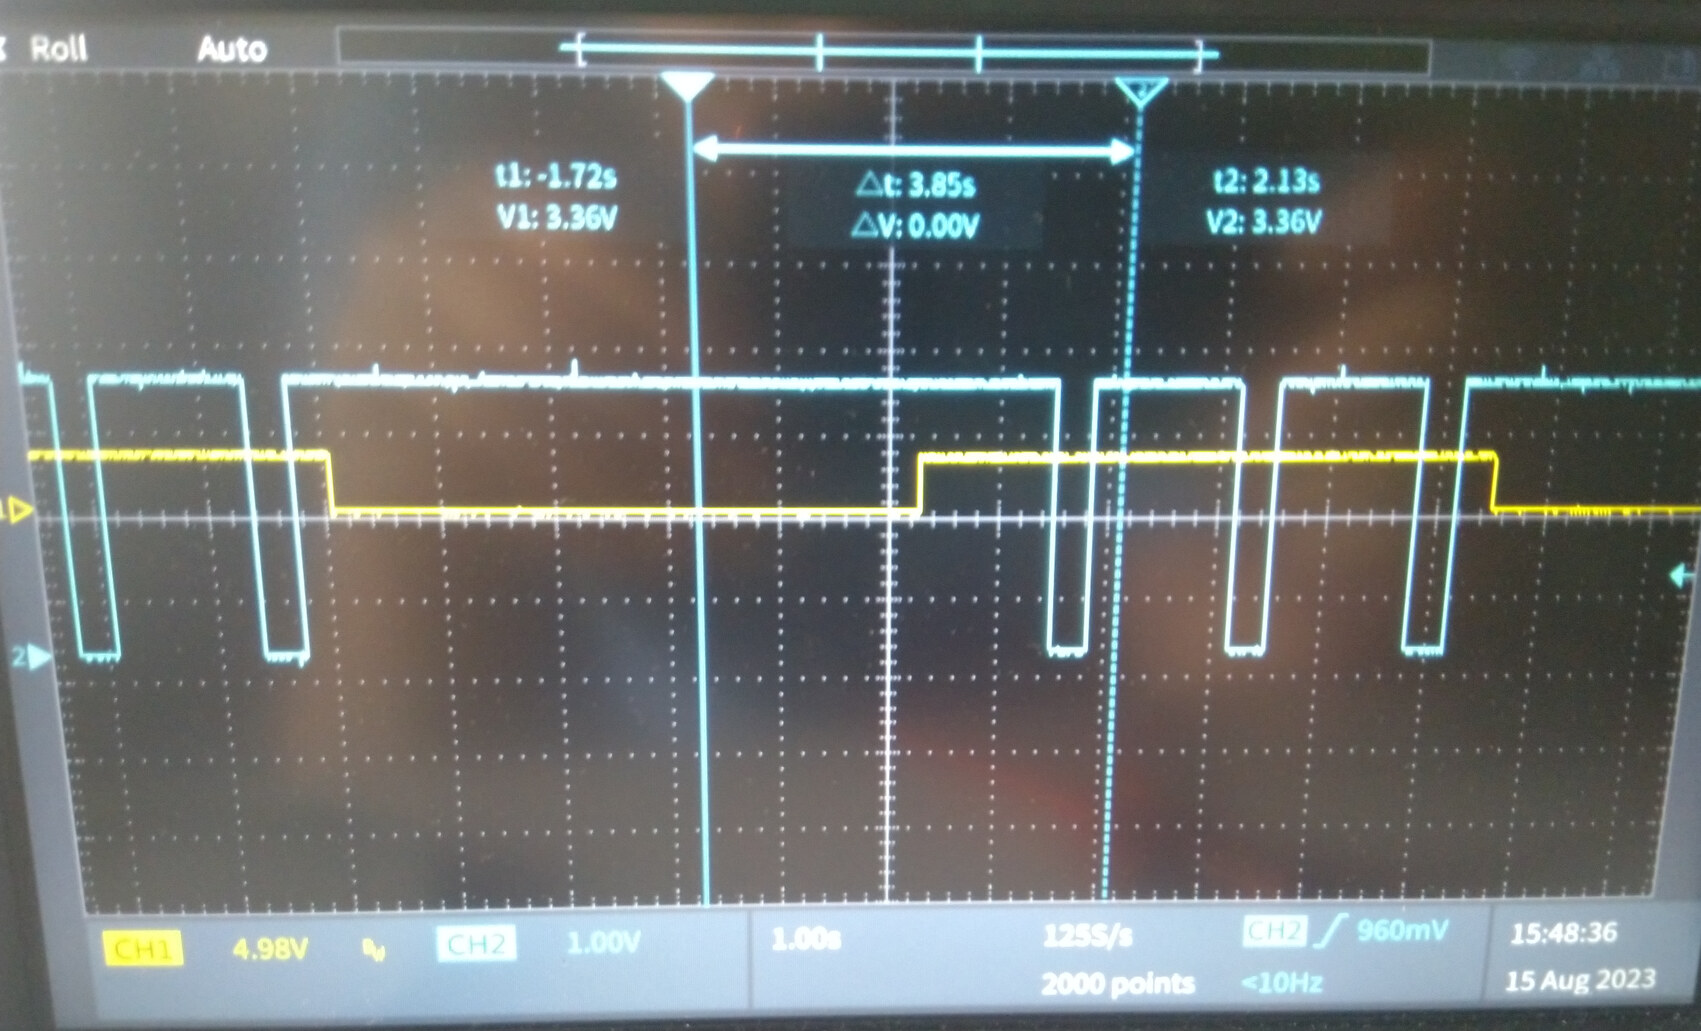
\includegraphics[width=0.9\textwidth]{watchdog_capture.jpg}
	\caption[Watchdog Reset Test on the Rev 0.0 Prototype]{Watchdog reset test on the inherited Rev~0.0 prototype (oscilloscope date stamp 15~August~2023). A test design in the \gls{fpga} toggles the watchdog service line about every \SI{20}{\milli\second} for about five seconds (256 times) and then withholds service, so that the watchdog pulls the controller reset low; Leyer expected a reset every \SI{1.2}{\second} and doubted the value~\cite[Sec.~4.6]{leyer2023}. Read from the photograph, the first reset follows about \SI{1.2}{\second} after the service stops, and resets of about \SI{0.3}{\second} recur about \SI{1.6}{\second} apart (\Cref{subsec:fpga_interface_results}). Yellow: service line, inverted before the watchdog (the individual pulses are not resolved); blue: controller reset line. The cursor readout ($\Delta t = \SI{3.85}{\second}$, \SI{3.36}{\volt}) measures no watchdog parameter; the voltage is the cursor level. Reproduced from~\cite[Fig.~9]{leyer2023}, cropped to the screen from the archived photograph.}
	\label{fig:watchdog_reaction}
\end{figure}

% ============================================================
% Appendix D: YAML Test Cases and VHDL Excerpt
% ============================================================
\chapter{YAML Test Cases and VHDL Excerpt}
\label{app:test_cases}

This appendix provides illustrative examples of the test definition files and the \gls{vhdl} design used during the verification and validation process, as detailed in \Cref{chap:testing}.

% ------------------------------------------------------------
\section{YAML Test Case Definitions for Fixture-Based Testing}
\label{sec:app_yaml_test_cases}

System-level scenario testing (\Cref{sec:system_scenario_testing}) was driven by sequences defined in \gls{yaml} format and executed via the test fixture~\cite{dolata2023}. The structure allows for the definition of input pin states, expected outputs, and tester interactions.

\subsection*{Example Test Case: Geber 3 Fault Handling}
The following test case, adapted from~\cite[Listing~3]{dolata2023}, illustrates the two-step verification sequence for a \enquote{Geber 3} fault; the longer descriptions and the comments were added:

{\footnotesize
\begin{verbatim}
# Test group for Geber 3 fault simulation
- name: Geber 3 - I
  description: >-
    Test für den Geber. Bitte 3 Sekunden warten,
    bis der Fehler angezeigt wird. Danach STW
    gedrückt halten und Fehlersequenz überprüfen.
  pin_sets: {18z: 1, 24d: 0} # Simulate fault
  expected_err_code: "31"    # Fixture: 31; manual: 03
  expected_err_seq: "03 31 09" # Expect seq on STW
  del: False                 # No 'Loesch' prompt

- name: Geber 3 - II
  description: STW gedrückt halten und Fehlersequenz überprüfen.
  pin_sets: {}               # Fault no longer applied
  expected_err_code: "95"    # Expect '95': sporadic fault
  expected_err_seq: "03 31 09" # Re-verify seq
  del: True                  # Prompt 'Loesch'
\end{verbatim}
}

The code 31 that the first step expects on the display is the fixture's expectation; the manual and the table of the fixture report give 03 for this display (\Cref{tab:requirement_basis}, note~b), and the sources do not explain the difference. In the second step the fault is no longer applied, and the display is expected to show 95, the code of a sporadic fault, one that occurred and is no longer active~\cite[Tab.~2, Sec.~9.3]{dolata2023}; Leyer describes it as a temporary error~\cite[Sec.~5.1.3]{leyer2023}.

% ------------------------------------------------------------
\section{VHDL Excerpt: NVRAM Control}
\label{sec:app_vhdl_testbenches}

The following excerpt from the top-level design \texttt{atop.vhd} shows the \gls{nvram} control assignments in the version archived with Leyer's documentation in September 2023 (project \texttt{TestDiagnose\_new})~\cite{leyer2023}, with the original line numbers; in the simulated project the same assignment stands in line~473. Line~513 contains defect~B1 (\Cref{tab:bug_taxonomy}): the byte-low enable \texttt{NVRAM\_ble} is held high, so the 8-bit data path (\texttt{NVRAM\_dq}, bits 7 to 0) never reaches the memory. The follow-on project corrected the assignment to \texttt{\textquotesingle 0\textquotesingle}, which enables the lower byte permanently~\cite[pp.~14--15]{savchuk2025}.

{\footnotesize
\begin{verbatim}
510      -- nvram
511      --
512      --NVRAM_add <= dmem_addr_os (5 downto 0);
513      NVRAM_ble <= '1';
514      NVRAM_oe <= rd_n_os;
515      NVRAM_ce_s <= not ((not (rd_n_os or p27)) or (not (p27 or wr_n_os)));
516      NVRAM_ce <= NVRAM_ce_s;
517      NVRAM_we <= wr_n_os;
518      -- dmem_data_is <= NVRAM_dq;
519      NVRAM_ctrl (2) <= p2_os(7);
520      NVRAM_ctrl (1) <= wr_n_os;
521      NVRAM_ctrl (0) <= NVRAM_ce_s;
\end{verbatim}
}

\clearpage

% --- BACK MATTER ---
\backmatter
\pagestyle{fancy}

% Ragged right: the long URLs and the standard numbers kept on one line left loose,
% letterspaced lines in a justified list, and no local emergency stretch removed them
% without overfull lines
{\raggedright\printbibliography[title=References, heading=bibintoc]\par}
\clearpage

\end{document}
